% Options for packages loaded elsewhere
\PassOptionsToPackage{unicode}{hyperref}
\PassOptionsToPackage{hyphens}{url}
%
\documentclass[
]{article}
\usepackage{amsmath,amssymb}
\usepackage{lmodern}
\usepackage{iftex}
\ifPDFTeX
  \usepackage[T1]{fontenc}
  \usepackage[utf8]{inputenc}
  \usepackage{textcomp} % provide euro and other symbols
\else % if luatex or xetex
  \usepackage{unicode-math}
  \defaultfontfeatures{Scale=MatchLowercase}
  \defaultfontfeatures[\rmfamily]{Ligatures=TeX,Scale=1}
\fi
% Use upquote if available, for straight quotes in verbatim environments
\IfFileExists{upquote.sty}{\usepackage{upquote}}{}
\IfFileExists{microtype.sty}{% use microtype if available
  \usepackage[]{microtype}
  \UseMicrotypeSet[protrusion]{basicmath} % disable protrusion for tt fonts
}{}
\makeatletter
\@ifundefined{KOMAClassName}{% if non-KOMA class
  \IfFileExists{parskip.sty}{%
    \usepackage{parskip}
  }{% else
    \setlength{\parindent}{0pt}
    \setlength{\parskip}{6pt plus 2pt minus 1pt}}
}{% if KOMA class
  \KOMAoptions{parskip=half}}
\makeatother
\usepackage{xcolor}
\usepackage[margin=1in]{geometry}
\usepackage{color}
\usepackage{fancyvrb}
\newcommand{\VerbBar}{|}
\newcommand{\VERB}{\Verb[commandchars=\\\{\}]}
\DefineVerbatimEnvironment{Highlighting}{Verbatim}{commandchars=\\\{\}}
% Add ',fontsize=\small' for more characters per line
\usepackage{framed}
\definecolor{shadecolor}{RGB}{248,248,248}
\newenvironment{Shaded}{\begin{snugshade}}{\end{snugshade}}
\newcommand{\AlertTok}[1]{\textcolor[rgb]{0.94,0.16,0.16}{#1}}
\newcommand{\AnnotationTok}[1]{\textcolor[rgb]{0.56,0.35,0.01}{\textbf{\textit{#1}}}}
\newcommand{\AttributeTok}[1]{\textcolor[rgb]{0.77,0.63,0.00}{#1}}
\newcommand{\BaseNTok}[1]{\textcolor[rgb]{0.00,0.00,0.81}{#1}}
\newcommand{\BuiltInTok}[1]{#1}
\newcommand{\CharTok}[1]{\textcolor[rgb]{0.31,0.60,0.02}{#1}}
\newcommand{\CommentTok}[1]{\textcolor[rgb]{0.56,0.35,0.01}{\textit{#1}}}
\newcommand{\CommentVarTok}[1]{\textcolor[rgb]{0.56,0.35,0.01}{\textbf{\textit{#1}}}}
\newcommand{\ConstantTok}[1]{\textcolor[rgb]{0.00,0.00,0.00}{#1}}
\newcommand{\ControlFlowTok}[1]{\textcolor[rgb]{0.13,0.29,0.53}{\textbf{#1}}}
\newcommand{\DataTypeTok}[1]{\textcolor[rgb]{0.13,0.29,0.53}{#1}}
\newcommand{\DecValTok}[1]{\textcolor[rgb]{0.00,0.00,0.81}{#1}}
\newcommand{\DocumentationTok}[1]{\textcolor[rgb]{0.56,0.35,0.01}{\textbf{\textit{#1}}}}
\newcommand{\ErrorTok}[1]{\textcolor[rgb]{0.64,0.00,0.00}{\textbf{#1}}}
\newcommand{\ExtensionTok}[1]{#1}
\newcommand{\FloatTok}[1]{\textcolor[rgb]{0.00,0.00,0.81}{#1}}
\newcommand{\FunctionTok}[1]{\textcolor[rgb]{0.00,0.00,0.00}{#1}}
\newcommand{\ImportTok}[1]{#1}
\newcommand{\InformationTok}[1]{\textcolor[rgb]{0.56,0.35,0.01}{\textbf{\textit{#1}}}}
\newcommand{\KeywordTok}[1]{\textcolor[rgb]{0.13,0.29,0.53}{\textbf{#1}}}
\newcommand{\NormalTok}[1]{#1}
\newcommand{\OperatorTok}[1]{\textcolor[rgb]{0.81,0.36,0.00}{\textbf{#1}}}
\newcommand{\OtherTok}[1]{\textcolor[rgb]{0.56,0.35,0.01}{#1}}
\newcommand{\PreprocessorTok}[1]{\textcolor[rgb]{0.56,0.35,0.01}{\textit{#1}}}
\newcommand{\RegionMarkerTok}[1]{#1}
\newcommand{\SpecialCharTok}[1]{\textcolor[rgb]{0.00,0.00,0.00}{#1}}
\newcommand{\SpecialStringTok}[1]{\textcolor[rgb]{0.31,0.60,0.02}{#1}}
\newcommand{\StringTok}[1]{\textcolor[rgb]{0.31,0.60,0.02}{#1}}
\newcommand{\VariableTok}[1]{\textcolor[rgb]{0.00,0.00,0.00}{#1}}
\newcommand{\VerbatimStringTok}[1]{\textcolor[rgb]{0.31,0.60,0.02}{#1}}
\newcommand{\WarningTok}[1]{\textcolor[rgb]{0.56,0.35,0.01}{\textbf{\textit{#1}}}}
\usepackage{longtable,booktabs,array}
\usepackage{calc} % for calculating minipage widths
% Correct order of tables after \paragraph or \subparagraph
\usepackage{etoolbox}
\makeatletter
\patchcmd\longtable{\par}{\if@noskipsec\mbox{}\fi\par}{}{}
\makeatother
% Allow footnotes in longtable head/foot
\IfFileExists{footnotehyper.sty}{\usepackage{footnotehyper}}{\usepackage{footnote}}
\makesavenoteenv{longtable}
\usepackage{graphicx}
\makeatletter
\def\maxwidth{\ifdim\Gin@nat@width>\linewidth\linewidth\else\Gin@nat@width\fi}
\def\maxheight{\ifdim\Gin@nat@height>\textheight\textheight\else\Gin@nat@height\fi}
\makeatother
% Scale images if necessary, so that they will not overflow the page
% margins by default, and it is still possible to overwrite the defaults
% using explicit options in \includegraphics[width, height, ...]{}
\setkeys{Gin}{width=\maxwidth,height=\maxheight,keepaspectratio}
% Set default figure placement to htbp
\makeatletter
\def\fps@figure{htbp}
\makeatother
\setlength{\emergencystretch}{3em} % prevent overfull lines
\providecommand{\tightlist}{%
  \setlength{\itemsep}{0pt}\setlength{\parskip}{0pt}}
\setcounter{secnumdepth}{-\maxdimen} % remove section numbering
\ifLuaTeX
  \usepackage{selnolig}  % disable illegal ligatures
\fi
\IfFileExists{bookmark.sty}{\usepackage{bookmark}}{\usepackage{hyperref}}
\IfFileExists{xurl.sty}{\usepackage{xurl}}{} % add URL line breaks if available
\urlstyle{same} % disable monospaced font for URLs
\hypersetup{
  pdftitle={P8108 Final Project},
  hidelinks,
  pdfcreator={LaTeX via pandoc}}

\title{P8108 Final Project}
\author{}
\date{\vspace{-2.5em}2022-11-28}

\begin{document}
\maketitle

\hypertarget{import-dataset-and-data-preprocess}{%
\subsection{1 Import Dataset and Data
Preprocess}\label{import-dataset-and-data-preprocess}}

\begin{Shaded}
\begin{Highlighting}[]
\FunctionTok{data}\NormalTok{(cancer, }\AttributeTok{package=}\StringTok{"survival"}\NormalTok{)}

\NormalTok{lung\_df}\OtherTok{=}\NormalTok{lung}

\NormalTok{lung\_df }\OtherTok{=}\NormalTok{ lung\_df }\SpecialCharTok{\%\textgreater{}\%}
  \FunctionTok{mutate}\NormalTok{(}\AttributeTok{status =} \FunctionTok{case\_when}\NormalTok{(status }\SpecialCharTok{==} \DecValTok{1} \SpecialCharTok{\textasciitilde{}} \DecValTok{0}\NormalTok{,}
\NormalTok{                            status }\SpecialCharTok{==} \DecValTok{2} \SpecialCharTok{\textasciitilde{}} \DecValTok{1}\NormalTok{)) }\SpecialCharTok{\%\textgreater{}\%}
  \FunctionTok{mutate}\NormalTok{(}\AttributeTok{sex =} \FunctionTok{as.factor}\NormalTok{(sex),}
         \AttributeTok{ph.ecog =} \FunctionTok{as.factor}\NormalTok{(ph.ecog), }
         \AttributeTok{status =} \FunctionTok{as.factor}\NormalTok{(status))}
\end{Highlighting}
\end{Shaded}

\hypertarget{exploratory-analysis}{%
\subsection{2 Exploratory Analysis}\label{exploratory-analysis}}

\hypertarget{summary-table}{%
\subsubsection{2.1 Summary table}\label{summary-table}}

\begin{Shaded}
\begin{Highlighting}[]
\CommentTok{\# Metadata Title}
\NormalTok{DATASET }\OtherTok{\textless{}{-}} \FunctionTok{paste0}\NormalTok{(}\StringTok{"NCCTG Lung Cancer Dataset (from survival package "}\NormalTok{, }
                  \FunctionTok{packageVersion}\NormalTok{(}\StringTok{"survival"}\NormalTok{), }\StringTok{")"}\NormalTok{)}

\CommentTok{\# Save original options()}
\NormalTok{old }\OtherTok{\textless{}{-}} \FunctionTok{options}\NormalTok{()  }

\CommentTok{\# Global formatting options}
\FunctionTok{options}\NormalTok{(}\AttributeTok{digits =} \DecValTok{3}\NormalTok{)}

\CommentTok{\# Global ggplot settings}
\FunctionTok{theme\_set}\NormalTok{(}\FunctionTok{theme\_bw}\NormalTok{())}

\CommentTok{\# Global table settings }
\FunctionTok{options}\NormalTok{(}\AttributeTok{DT.options =} \FunctionTok{list}\NormalTok{(}\AttributeTok{pageLength =} \DecValTok{10}\NormalTok{, }
                          \AttributeTok{language =} \FunctionTok{list}\NormalTok{(}\AttributeTok{search =} \StringTok{\textquotesingle{}Filter:\textquotesingle{}}\NormalTok{), }
                          \AttributeTok{scrollX =} \ConstantTok{TRUE}\NormalTok{))}

\CommentTok{\# Restore original options()}
\FunctionTok{options}\NormalTok{(old)}
\end{Highlighting}
\end{Shaded}

\begin{Shaded}
\begin{Highlighting}[]
\FunctionTok{str}\NormalTok{(lung\_df)}
\end{Highlighting}
\end{Shaded}

\begin{verbatim}
## 'data.frame':    228 obs. of  10 variables:
##  $ inst     : num  3 3 3 5 1 12 7 11 1 7 ...
##  $ time     : num  306 455 1010 210 883 ...
##  $ status   : Factor w/ 2 levels "0","1": 2 2 1 2 2 1 2 2 2 2 ...
##  $ age      : num  74 68 56 57 60 74 68 71 53 61 ...
##  $ sex      : Factor w/ 2 levels "1","2": 1 1 1 1 1 1 2 2 1 1 ...
##  $ ph.ecog  : Factor w/ 4 levels "0","1","2","3": 2 1 1 2 1 2 3 3 2 3 ...
##  $ ph.karno : num  90 90 90 90 100 50 70 60 70 70 ...
##  $ pat.karno: num  100 90 90 60 90 80 60 80 80 70 ...
##  $ meal.cal : num  1175 1225 NA 1150 NA ...
##  $ wt.loss  : num  NA 15 15 11 0 0 10 1 16 34 ...
\end{verbatim}

\begin{Shaded}
\begin{Highlighting}[]
\CommentTok{\# Select variables of interest and change names to look nicer}
\NormalTok{lung\_tab }\OtherTok{\textless{}{-}}\NormalTok{ lung\_df }\SpecialCharTok{\%\textgreater{}\%}  
\NormalTok{  dplyr}\SpecialCharTok{::}\FunctionTok{select}\NormalTok{(age, sex, status, ph.ecog, ph.karno, pat.karno, meal.cal, wt.loss) }\SpecialCharTok{\%\textgreater{}\%}
  \FunctionTok{mutate}\NormalTok{(}\AttributeTok{sex =} \FunctionTok{case\_when}\NormalTok{(sex }\SpecialCharTok{==} \DecValTok{1} \SpecialCharTok{\textasciitilde{}} \StringTok{"Male"}\NormalTok{,}
\NormalTok{                         sex }\SpecialCharTok{==} \DecValTok{2} \SpecialCharTok{\textasciitilde{}} \StringTok{"Female"}\NormalTok{)) }\SpecialCharTok{\%\textgreater{}\%}
  \FunctionTok{mutate}\NormalTok{(}\AttributeTok{status =} \FunctionTok{case\_when}\NormalTok{(status }\SpecialCharTok{==} \DecValTok{0} \SpecialCharTok{\textasciitilde{}} \StringTok{"Censored"}\NormalTok{,}
\NormalTok{                            status }\SpecialCharTok{==} \DecValTok{1} \SpecialCharTok{\textasciitilde{}} \StringTok{"Dead"}\NormalTok{)) }\SpecialCharTok{\%\textgreater{}\%}
  \FunctionTok{mutate}\NormalTok{(}\AttributeTok{sex =} \FunctionTok{as.factor}\NormalTok{(sex),}
         \AttributeTok{ph.ecog =} \FunctionTok{as.factor}\NormalTok{(ph.ecog), }
         \AttributeTok{status =} \FunctionTok{as.factor}\NormalTok{(status)) }\SpecialCharTok{\%\textgreater{}\%}
  \FunctionTok{rename}\NormalTok{(}\StringTok{"Age"} \OtherTok{=} \StringTok{"age"}\NormalTok{, }
         \StringTok{"Sex"} \OtherTok{=} \StringTok{"sex"}\NormalTok{, }
         \StringTok{"Censoring Status"} \OtherTok{=} \StringTok{"status"}\NormalTok{, }
         \StringTok{"ECOG Performance Score"} \OtherTok{=} \StringTok{"ph.ecog"}\NormalTok{, }
         \StringTok{"Karnofsky Performance Score Rated by Physician"} \OtherTok{=} \StringTok{"ph.karno"}\NormalTok{, }
         \StringTok{"Karnofsky Performance Score Rated by Patient"} \OtherTok{=} \StringTok{"pat.karno"}\NormalTok{, }
         \StringTok{"Calories Consumed at Meals"} \OtherTok{=} \StringTok{"meal.cal"}\NormalTok{, }
         \StringTok{"Weight Loss in Last Six Months"}\OtherTok{=}\StringTok{"wt.loss"}\NormalTok{) }

\CommentTok{\# Create a table one}
\NormalTok{tab1 }\OtherTok{\textless{}{-}} \FunctionTok{get\_tableone}\NormalTok{(lung\_tab)}

\CommentTok{\# Render the tableone}
\NormalTok{table1 }\OtherTok{=} \FunctionTok{render}\NormalTok{(tab1, }\AttributeTok{title =} \StringTok{"Overview over Lung Cancer patients"}\NormalTok{, }\AttributeTok{datasource =}\NormalTok{ DATASET)}
\end{Highlighting}
\end{Shaded}

\hypertarget{distribution-plots-for-each-variable}{%
\subsubsection{2.2 Distribution plots for each
variable}\label{distribution-plots-for-each-variable}}

\begin{Shaded}
\begin{Highlighting}[]
\CommentTok{\# Pie chart}
\DocumentationTok{\#\# Gender{-}pie chart}
\NormalTok{lung\_df\_pie\_1 }\OtherTok{=} 
\NormalTok{  lung\_df }\SpecialCharTok{\%\textgreater{}\%} 
  \FunctionTok{group\_by}\NormalTok{(sex) }\SpecialCharTok{\%\textgreater{}\%} 
  \FunctionTok{count}\NormalTok{() }\SpecialCharTok{\%\textgreater{}\%} 
  \FunctionTok{mutate}\NormalTok{(}\AttributeTok{total\_n =} \FunctionTok{c}\NormalTok{(}\DecValTok{138} \SpecialCharTok{+} \DecValTok{90}\NormalTok{)) }\SpecialCharTok{\%\textgreater{}\%} 
  \FunctionTok{mutate}\NormalTok{(}\AttributeTok{perc =} \StringTok{\textasciigrave{}}\AttributeTok{n}\StringTok{\textasciigrave{}} \SpecialCharTok{/} \StringTok{\textasciigrave{}}\AttributeTok{total\_n}\StringTok{\textasciigrave{}}\NormalTok{) }\SpecialCharTok{\%\textgreater{}\%} 
  \FunctionTok{arrange}\NormalTok{(perc) }\SpecialCharTok{\%\textgreater{}\%}
  \FunctionTok{mutate}\NormalTok{(}\AttributeTok{labels =}\NormalTok{ scales}\SpecialCharTok{::}\FunctionTok{percent}\NormalTok{(perc, }\FloatTok{0.01}\NormalTok{)) }\SpecialCharTok{\%\textgreater{}\%}
  \FunctionTok{mutate}\NormalTok{(}\AttributeTok{Sex =} \FunctionTok{case\_when}\NormalTok{(sex }\SpecialCharTok{==} \DecValTok{1} \SpecialCharTok{\textasciitilde{}} \StringTok{"Male"}\NormalTok{,}
\NormalTok{                         sex }\SpecialCharTok{==} \DecValTok{2} \SpecialCharTok{\textasciitilde{}} \StringTok{"Female"}\NormalTok{)) }
\NormalTok{p\_gender }\OtherTok{=}
  \FunctionTok{ggplot}\NormalTok{(lung\_df\_pie\_1, }\FunctionTok{aes}\NormalTok{(}\AttributeTok{x=}\StringTok{""}\NormalTok{, }\AttributeTok{y=}\NormalTok{perc, }\AttributeTok{fill=}\NormalTok{Sex)) }\SpecialCharTok{+} 
  \FunctionTok{geom\_bar}\NormalTok{(}\AttributeTok{width =} \DecValTok{1}\NormalTok{, }\AttributeTok{stat =} \StringTok{"identity"}\NormalTok{, }\AttributeTok{color=}\StringTok{"white"}\NormalTok{, }\AttributeTok{alpha =} \FloatTok{0.7}\NormalTok{) }\SpecialCharTok{+} 
  \FunctionTok{geom\_label}\NormalTok{(}\FunctionTok{aes}\NormalTok{(}\AttributeTok{label =}\NormalTok{ labels),}
             \AttributeTok{position =} \FunctionTok{position\_stack}\NormalTok{(}\AttributeTok{vjust =} \FloatTok{0.5}\NormalTok{),}
             \AttributeTok{show.legend =} \ConstantTok{FALSE}\NormalTok{,}
             \AttributeTok{color =} \StringTok{"white"}\NormalTok{) }\SpecialCharTok{+}
  \FunctionTok{coord\_polar}\NormalTok{(}\StringTok{"y"}\NormalTok{, }\AttributeTok{start=}\DecValTok{0}\NormalTok{) }\SpecialCharTok{+}
  \FunctionTok{scale\_fill\_brewer}\NormalTok{(}\AttributeTok{palette=}\StringTok{"Set2"}\NormalTok{) }\SpecialCharTok{+}
  \FunctionTok{theme\_void}\NormalTok{() }\SpecialCharTok{+}
  \FunctionTok{guides}\NormalTok{(}\AttributeTok{fill =} \FunctionTok{guide\_legend}\NormalTok{(}\AttributeTok{title =} \StringTok{"Sex"}\NormalTok{)) }

\DocumentationTok{\#\# ECOG{-}pie chart}
\NormalTok{lung\_df\_pie\_2 }\OtherTok{=}\NormalTok{ lung\_df }\SpecialCharTok{\%\textgreater{}\%} 
  \FunctionTok{group\_by}\NormalTok{(ph.ecog) }\SpecialCharTok{\%\textgreater{}\%} 
  \FunctionTok{count}\NormalTok{() }\SpecialCharTok{\%\textgreater{}\%} 
  \FunctionTok{mutate}\NormalTok{(}\AttributeTok{total\_n =} \FunctionTok{c}\NormalTok{(}\DecValTok{63} \SpecialCharTok{+} \DecValTok{113} \SpecialCharTok{+} \DecValTok{50} \SpecialCharTok{+} \DecValTok{1} \SpecialCharTok{+} \DecValTok{1}\NormalTok{)) }\SpecialCharTok{\%\textgreater{}\%} 
  \FunctionTok{mutate}\NormalTok{(}\AttributeTok{perc =} \StringTok{\textasciigrave{}}\AttributeTok{n}\StringTok{\textasciigrave{}} \SpecialCharTok{/} \StringTok{\textasciigrave{}}\AttributeTok{total\_n}\StringTok{\textasciigrave{}}\NormalTok{) }\SpecialCharTok{\%\textgreater{}\%} 
  \FunctionTok{arrange}\NormalTok{(perc) }\SpecialCharTok{\%\textgreater{}\%}
  \FunctionTok{mutate}\NormalTok{(}\AttributeTok{labels =}\NormalTok{ scales}\SpecialCharTok{::}\FunctionTok{percent}\NormalTok{(perc, }\FloatTok{0.01}\NormalTok{)) }\SpecialCharTok{\%\textgreater{}\%}
  \FunctionTok{as.data.frame}\NormalTok{() }\SpecialCharTok{\%\textgreater{}\%}
  \FunctionTok{mutate}\NormalTok{(}\AttributeTok{ph.ecog =} \FunctionTok{as.character}\NormalTok{(ph.ecog)) }
         
\NormalTok{lung\_df\_pie\_2[}\FunctionTok{is.na}\NormalTok{(lung\_df\_pie\_2)] }\OtherTok{=} \StringTok{"Missing"}
\NormalTok{p\_ecog }\OtherTok{=} 
  \FunctionTok{ggplot}\NormalTok{(lung\_df\_pie\_2, }\FunctionTok{aes}\NormalTok{(}\AttributeTok{x=}\StringTok{""}\NormalTok{, }\AttributeTok{y=}\NormalTok{perc, }\AttributeTok{fill=}\NormalTok{ph.ecog)) }\SpecialCharTok{+} 
  \FunctionTok{geom\_bar}\NormalTok{(}\AttributeTok{width =} \DecValTok{1}\NormalTok{, }\AttributeTok{stat =} \StringTok{"identity"}\NormalTok{, }\AttributeTok{color=}\StringTok{"white"}\NormalTok{, }\AttributeTok{alpha =} \FloatTok{0.7}\NormalTok{) }\SpecialCharTok{+} 
  \FunctionTok{geom\_label}\NormalTok{(}\FunctionTok{aes}\NormalTok{(}\AttributeTok{label =}\NormalTok{ labels),}
             \AttributeTok{position =} \FunctionTok{position\_stack}\NormalTok{(}\AttributeTok{vjust =} \FloatTok{0.5}\NormalTok{),}
             \AttributeTok{show.legend =} \ConstantTok{FALSE}\NormalTok{,}
             \AttributeTok{color =} \StringTok{"white"}\NormalTok{) }\SpecialCharTok{+}
  \FunctionTok{coord\_polar}\NormalTok{(}\StringTok{"y"}\NormalTok{, }\AttributeTok{start=}\DecValTok{0}\NormalTok{) }\SpecialCharTok{+}
  \FunctionTok{scale\_fill\_brewer}\NormalTok{(}\AttributeTok{palette=}\StringTok{"Set2"}\NormalTok{) }\SpecialCharTok{+}
  \FunctionTok{theme\_void}\NormalTok{() }\SpecialCharTok{+}
  \FunctionTok{guides}\NormalTok{(}\AttributeTok{fill =} \FunctionTok{guide\_legend}\NormalTok{(}\AttributeTok{title =} \StringTok{"ECOG Score"}\NormalTok{))}

\DocumentationTok{\#\# Status{-}pie chart}
\NormalTok{lung\_df\_pie\_3 }\OtherTok{=}\NormalTok{ lung\_df }\SpecialCharTok{\%\textgreater{}\%}
  \FunctionTok{group\_by}\NormalTok{(status) }\SpecialCharTok{\%\textgreater{}\%} 
  \FunctionTok{count}\NormalTok{() }\SpecialCharTok{\%\textgreater{}\%} 
  \FunctionTok{mutate}\NormalTok{(}\AttributeTok{total\_n =} \FunctionTok{c}\NormalTok{(}\DecValTok{63} \SpecialCharTok{+} \DecValTok{165}\NormalTok{)) }\SpecialCharTok{\%\textgreater{}\%} 
  \FunctionTok{mutate}\NormalTok{(}\AttributeTok{perc =} \StringTok{\textasciigrave{}}\AttributeTok{n}\StringTok{\textasciigrave{}} \SpecialCharTok{/} \StringTok{\textasciigrave{}}\AttributeTok{total\_n}\StringTok{\textasciigrave{}}\NormalTok{) }\SpecialCharTok{\%\textgreater{}\%} 
  \FunctionTok{arrange}\NormalTok{(perc) }\SpecialCharTok{\%\textgreater{}\%}
  \FunctionTok{mutate}\NormalTok{(}\AttributeTok{labels =}\NormalTok{ scales}\SpecialCharTok{::}\FunctionTok{percent}\NormalTok{(perc, }\FloatTok{0.01}\NormalTok{)) }\SpecialCharTok{\%\textgreater{}\%}
  \FunctionTok{mutate}\NormalTok{(}\AttributeTok{Status =} \FunctionTok{case\_when}\NormalTok{(status }\SpecialCharTok{==} \DecValTok{1} \SpecialCharTok{\textasciitilde{}} \StringTok{"Dead"}\NormalTok{,}
\NormalTok{                         status }\SpecialCharTok{==} \DecValTok{0} \SpecialCharTok{\textasciitilde{}} \StringTok{"Censored"}\NormalTok{)) }\SpecialCharTok{\%\textgreater{}\%}
  \FunctionTok{as.data.frame}\NormalTok{() }\SpecialCharTok{\%\textgreater{}\%}
  \FunctionTok{mutate}\NormalTok{(}\AttributeTok{status =} \FunctionTok{as.character}\NormalTok{(status)) }
  
\NormalTok{p\_status }\OtherTok{=} 
  \FunctionTok{ggplot}\NormalTok{(lung\_df\_pie\_3, }\FunctionTok{aes}\NormalTok{(}\AttributeTok{x=}\StringTok{""}\NormalTok{, }\AttributeTok{y=}\NormalTok{perc, }\AttributeTok{fill=}\NormalTok{Status)) }\SpecialCharTok{+} 
  \FunctionTok{geom\_bar}\NormalTok{(}\AttributeTok{width =} \DecValTok{1}\NormalTok{, }\AttributeTok{stat =} \StringTok{"identity"}\NormalTok{, }\AttributeTok{color=}\StringTok{"white"}\NormalTok{, }\AttributeTok{alpha =} \FloatTok{0.7}\NormalTok{) }\SpecialCharTok{+} 
  \FunctionTok{geom\_label}\NormalTok{(}\FunctionTok{aes}\NormalTok{(}\AttributeTok{label =}\NormalTok{ labels),}
             \AttributeTok{position =} \FunctionTok{position\_stack}\NormalTok{(}\AttributeTok{vjust =} \FloatTok{0.5}\NormalTok{),}
             \AttributeTok{show.legend =} \ConstantTok{FALSE}\NormalTok{,}
             \AttributeTok{color =} \StringTok{"white"}\NormalTok{) }\SpecialCharTok{+}
  \FunctionTok{coord\_polar}\NormalTok{(}\StringTok{"y"}\NormalTok{, }\AttributeTok{start=}\DecValTok{0}\NormalTok{) }\SpecialCharTok{+}
  \FunctionTok{scale\_fill\_brewer}\NormalTok{(}\AttributeTok{palette=}\StringTok{"Set2"}\NormalTok{) }\SpecialCharTok{+}
  \FunctionTok{theme\_void}\NormalTok{() }\SpecialCharTok{+}
  \FunctionTok{guides}\NormalTok{(}\AttributeTok{fill =} \FunctionTok{guide\_legend}\NormalTok{(}\AttributeTok{title =} \StringTok{"Status"}\NormalTok{))}

\CommentTok{\# Histogram}
\DocumentationTok{\#\# Time}
\NormalTok{p\_time }\OtherTok{=} 
\NormalTok{  lung\_df }\SpecialCharTok{\%\textgreater{}\%}
  \FunctionTok{ggplot}\NormalTok{(}\FunctionTok{aes}\NormalTok{(}\AttributeTok{x =}\NormalTok{ time)) }\SpecialCharTok{+} 
  \FunctionTok{geom\_histogram}\NormalTok{(}\FunctionTok{aes}\NormalTok{(}\AttributeTok{y=}\FunctionTok{after\_stat}\NormalTok{(density)), }\AttributeTok{color=}\StringTok{"darkblue"}\NormalTok{, }\AttributeTok{fill=}\StringTok{"lightblue"}\NormalTok{) }\SpecialCharTok{+}
  \FunctionTok{geom\_density}\NormalTok{() }\SpecialCharTok{+}
  \FunctionTok{labs}\NormalTok{(}\AttributeTok{x=}\StringTok{"Survival Time (Days)"}\NormalTok{,}
       \AttributeTok{y =} \StringTok{"Density"}\NormalTok{)}

\DocumentationTok{\#\# Age}
\NormalTok{p\_age }\OtherTok{=} 
\NormalTok{  lung\_df }\SpecialCharTok{\%\textgreater{}\%}
  \FunctionTok{mutate}\NormalTok{(}\AttributeTok{Sex =} \FunctionTok{case\_when}\NormalTok{(sex }\SpecialCharTok{==} \DecValTok{1} \SpecialCharTok{\textasciitilde{}} \StringTok{"Male"}\NormalTok{,}
\NormalTok{                         sex }\SpecialCharTok{==} \DecValTok{2} \SpecialCharTok{\textasciitilde{}} \StringTok{"Female"}\NormalTok{)) }\SpecialCharTok{\%\textgreater{}\%}
  \FunctionTok{ggplot}\NormalTok{(}\FunctionTok{aes}\NormalTok{(}\AttributeTok{x =}\NormalTok{ age, }\AttributeTok{fill=}\NormalTok{Sex, }\AttributeTok{color =}\NormalTok{ Sex)) }\SpecialCharTok{+} 
  \FunctionTok{geom\_histogram}\NormalTok{(}\AttributeTok{position =} \StringTok{"identity"}\NormalTok{, }\AttributeTok{alpha =} \FloatTok{0.5}\NormalTok{) }\SpecialCharTok{+}
  \FunctionTok{labs}\NormalTok{(}\AttributeTok{x =} \StringTok{"Age"}\NormalTok{,}
       \AttributeTok{y =} \StringTok{"Count"}\NormalTok{)}

\DocumentationTok{\#\# ph.karno \& pat.karno}
\NormalTok{df\_karno }\OtherTok{=}\NormalTok{ lung\_df }\SpecialCharTok{\%\textgreater{}\%}
  \FunctionTok{rename}\NormalTok{(}\StringTok{"Patient"} \OtherTok{=}\NormalTok{ pat.karno,}
        \StringTok{"Physician"} \OtherTok{=}\NormalTok{ ph.karno) }\SpecialCharTok{\%\textgreater{}\%}
  \FunctionTok{pivot\_longer}\NormalTok{(}
\NormalTok{    Patient}\SpecialCharTok{:}\NormalTok{Physician,}
    \AttributeTok{names\_to =} \StringTok{"Rating"}\NormalTok{,}
    \AttributeTok{values\_to =} \StringTok{"Karnofsky"}
\NormalTok{  )}

\NormalTok{p\_karno }\OtherTok{=}
\NormalTok{  df\_karno }\SpecialCharTok{\%\textgreater{}\%}
  \FunctionTok{ggplot}\NormalTok{(}\FunctionTok{aes}\NormalTok{(}\AttributeTok{x=}\NormalTok{Karnofsky, }\AttributeTok{fill =}\NormalTok{ Rating, }\AttributeTok{color =}\NormalTok{ Rating)) }\SpecialCharTok{+} 
  \FunctionTok{geom\_histogram}\NormalTok{(}\AttributeTok{binwidth =} \DecValTok{10}\NormalTok{, }\AttributeTok{alpha=}\FloatTok{0.5}\NormalTok{, }\AttributeTok{position=}\StringTok{"identity"}\NormalTok{) }\SpecialCharTok{+} 
  \FunctionTok{labs}\NormalTok{(}\AttributeTok{x =} \StringTok{"Karnofsky Score"}\NormalTok{,}
       \AttributeTok{y =} \StringTok{"Count"}\NormalTok{)}

\DocumentationTok{\#\# Weight loss}
\NormalTok{p\_weight }\OtherTok{=}
\NormalTok{  lung\_df }\SpecialCharTok{\%\textgreater{}\%} \FunctionTok{ggplot}\NormalTok{(}\FunctionTok{aes}\NormalTok{(}\AttributeTok{x =}\NormalTok{ wt.loss)) }\SpecialCharTok{+} 
  \FunctionTok{geom\_histogram}\NormalTok{(}\FunctionTok{aes}\NormalTok{(}\AttributeTok{y=}\FunctionTok{after\_stat}\NormalTok{(density)), }\AttributeTok{color=}\StringTok{"darkblue"}\NormalTok{, }\AttributeTok{fill=}\StringTok{"lightblue"}\NormalTok{) }\SpecialCharTok{+}
  \FunctionTok{geom\_density}\NormalTok{() }\SpecialCharTok{+}
    \FunctionTok{labs}\NormalTok{(}\AttributeTok{x =} \StringTok{"Weight Loss (Lbs)"}\NormalTok{,}
       \AttributeTok{y =} \StringTok{"Density"}\NormalTok{)}
\DocumentationTok{\#\# Meal}
\NormalTok{p\_meal }\OtherTok{=}
\NormalTok{  lung\_df }\SpecialCharTok{\%\textgreater{}\%}
  \FunctionTok{ggplot}\NormalTok{(}\FunctionTok{aes}\NormalTok{(}\AttributeTok{x =}\NormalTok{ meal.cal)) }\SpecialCharTok{+} 
  \FunctionTok{geom\_histogram}\NormalTok{(}\FunctionTok{aes}\NormalTok{(}\AttributeTok{y=}\FunctionTok{after\_stat}\NormalTok{(density)), }\AttributeTok{color=}\StringTok{"darkblue"}\NormalTok{, }\AttributeTok{fill=}\StringTok{"lightblue"}\NormalTok{) }\SpecialCharTok{+}
  \FunctionTok{geom\_density}\NormalTok{() }\SpecialCharTok{+}
  \FunctionTok{labs}\NormalTok{(}\AttributeTok{x =} \StringTok{"Calories Consumed"}\NormalTok{,}
       \AttributeTok{y =} \StringTok{"Density"}\NormalTok{)}
\end{Highlighting}
\end{Shaded}

\begin{Shaded}
\begin{Highlighting}[]
\CommentTok{\# Combine}
\NormalTok{p\_gender  }\SpecialCharTok{+}\NormalTok{ p\_status }\SpecialCharTok{+}\NormalTok{ p\_ecog}
\end{Highlighting}
\end{Shaded}

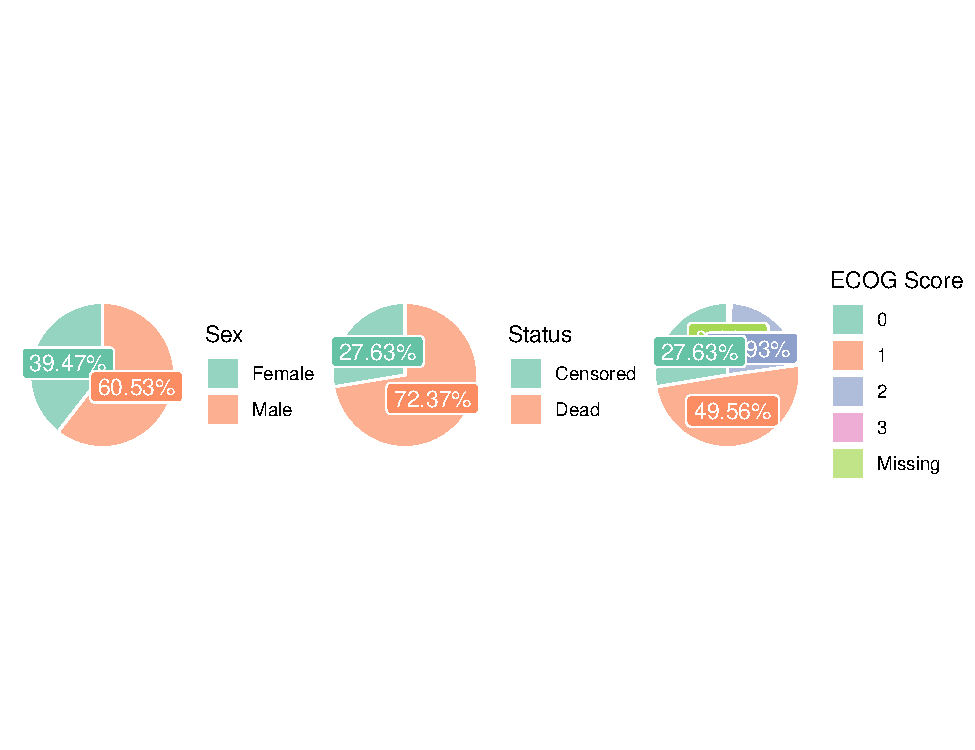
\includegraphics{final_project_files/figure-latex/unnamed-chunk-6-1.pdf}

\begin{Shaded}
\begin{Highlighting}[]
\NormalTok{p\_time }\SpecialCharTok{+}\NormalTok{ p\_weight }\SpecialCharTok{+}\NormalTok{ p\_meal}
\end{Highlighting}
\end{Shaded}

\begin{verbatim}
## `stat_bin()` using `bins = 30`. Pick better value with `binwidth`.
## `stat_bin()` using `bins = 30`. Pick better value with `binwidth`.
## `stat_bin()` using `bins = 30`. Pick better value with `binwidth`.
\end{verbatim}

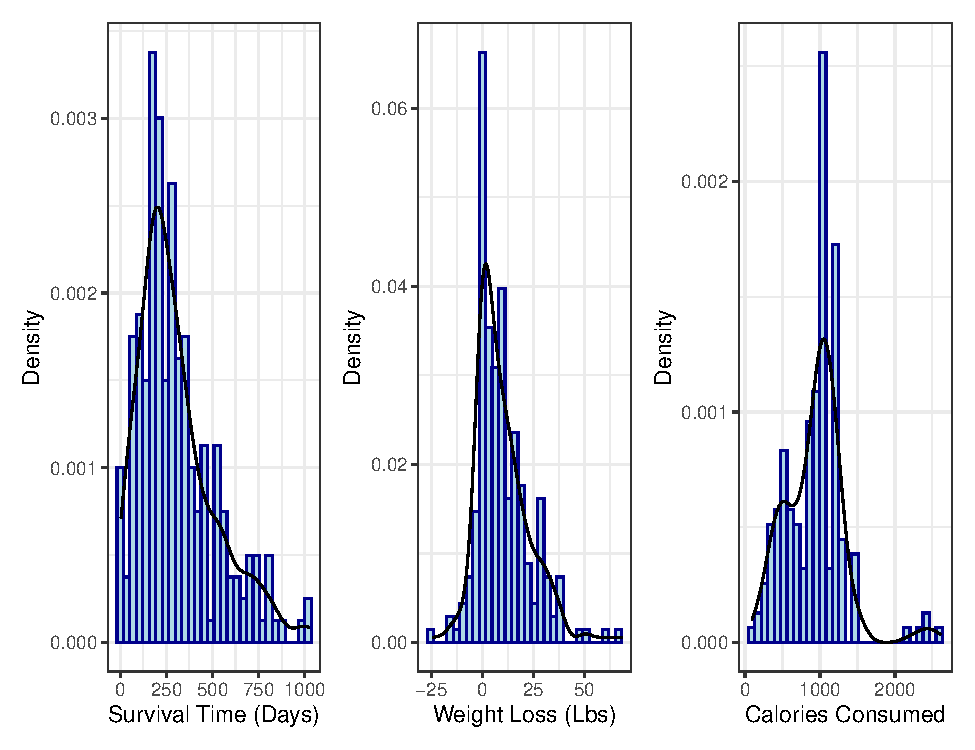
\includegraphics{final_project_files/figure-latex/unnamed-chunk-6-2.pdf}

\begin{Shaded}
\begin{Highlighting}[]
\NormalTok{p\_age }\SpecialCharTok{+}\NormalTok{ p\_karno}
\end{Highlighting}
\end{Shaded}

\begin{verbatim}
## `stat_bin()` using `bins = 30`. Pick better value with `binwidth`.
\end{verbatim}

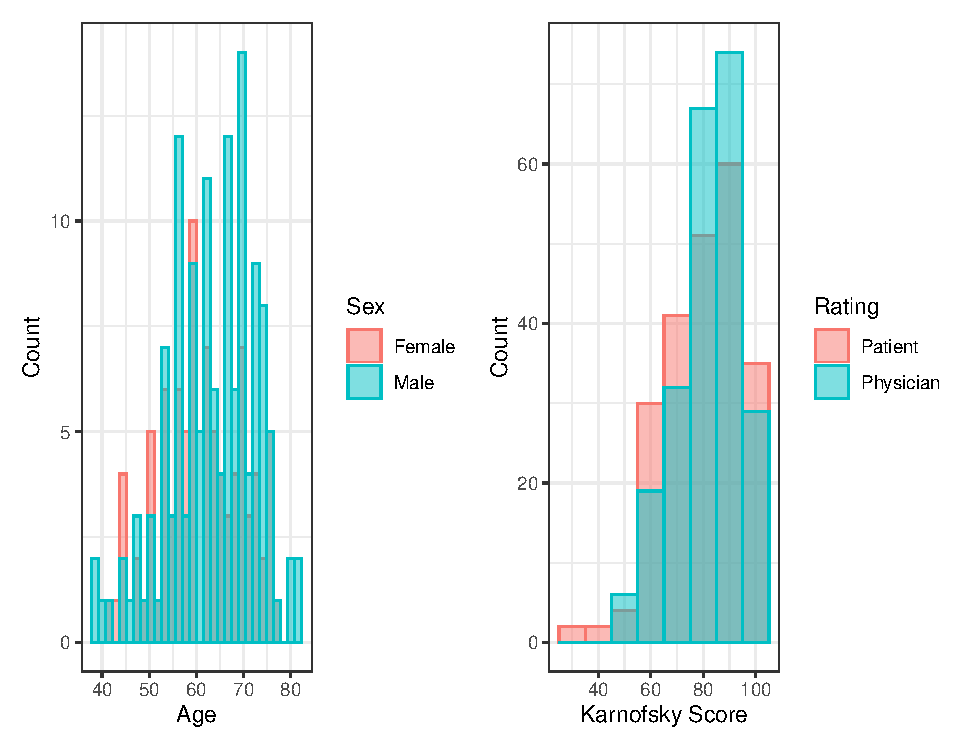
\includegraphics{final_project_files/figure-latex/unnamed-chunk-6-3.pdf}

\hypertarget{correlation-plot-between-variables}{%
\subsubsection{2.3 Correlation plot between
variables}\label{correlation-plot-between-variables}}

\begin{Shaded}
\begin{Highlighting}[]
\CommentTok{\# Drop missing values}
\NormalTok{lung\_df\_1 }\OtherTok{=}\NormalTok{ lung\_df }\SpecialCharTok{\%\textgreater{}\%}
  \FunctionTok{drop\_na}\NormalTok{()}

\CommentTok{\# Plot the correlation}
\NormalTok{corr }\OtherTok{=} \FunctionTok{data.frame}\NormalTok{(}\FunctionTok{lapply}\NormalTok{(}\FunctionTok{lapply}\NormalTok{(lung\_df\_1, as.factor), as.numeric))}
\FunctionTok{corrplot}\NormalTok{(}\FunctionTok{cor}\NormalTok{(corr), }\AttributeTok{type =} \StringTok{"lower"}\NormalTok{)}
\end{Highlighting}
\end{Shaded}

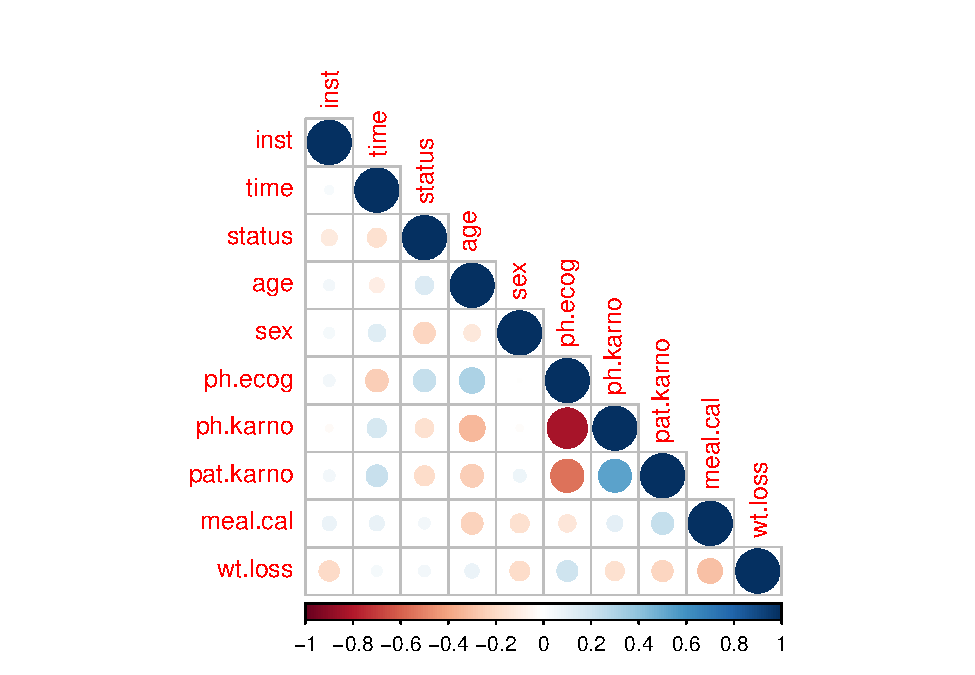
\includegraphics{final_project_files/figure-latex/unnamed-chunk-7-1.pdf}

\hypertarget{hazard-rate-summary-table}{%
\subsubsection{2.4 Hazard rate summary
table}\label{hazard-rate-summary-table}}

\begin{Shaded}
\begin{Highlighting}[]
\NormalTok{explanatory }\OtherTok{=} \FunctionTok{c}\NormalTok{(}\StringTok{"age"}\NormalTok{, }\StringTok{"sex"}\NormalTok{, }\StringTok{"ph.ecog"}\NormalTok{, }\StringTok{"ph.karno"}\NormalTok{, }\StringTok{"pat.karno"}\NormalTok{, }\StringTok{"meal.cal"}\NormalTok{, }\StringTok{"wt.loss"}\NormalTok{)}
\NormalTok{dependent }\OtherTok{=} \StringTok{"Surv(time, status)"}

\NormalTok{lung }\SpecialCharTok{\%\textgreater{}\%}
  \FunctionTok{mutate}\NormalTok{(}\AttributeTok{sex =} \FunctionTok{case\_when}\NormalTok{(sex }\SpecialCharTok{==} \DecValTok{2} \SpecialCharTok{\textasciitilde{}} \StringTok{"Female"}\NormalTok{,}
\NormalTok{                         sex }\SpecialCharTok{==} \DecValTok{1} \SpecialCharTok{\textasciitilde{}} \StringTok{"Male"}\NormalTok{)) }\SpecialCharTok{\%\textgreater{}\%}
  \FunctionTok{mutate}\NormalTok{(}\AttributeTok{ph.ecog =} \FunctionTok{ifelse}\NormalTok{(ph.ecog }\SpecialCharTok{==} \DecValTok{3}\NormalTok{, }\DecValTok{2}\NormalTok{, ph.ecog)) }\SpecialCharTok{\%\textgreater{}\%}
  \FunctionTok{mutate}\NormalTok{(}\AttributeTok{sex=}\FunctionTok{as.factor}\NormalTok{(sex), }
         \AttributeTok{ph.ecog=}\FunctionTok{as.factor}\NormalTok{(ph.ecog)) }\SpecialCharTok{\%\textgreater{}\%}
  \FunctionTok{hr\_plot}\NormalTok{(dependent, }
\NormalTok{          explanatory, }
          \AttributeTok{dependent\_label =} \StringTok{"Survival"}\NormalTok{,}
          \AttributeTok{remove\_ref =} \ConstantTok{FALSE}\NormalTok{,}
          \AttributeTok{table\_text\_size=}\DecValTok{4}\NormalTok{, }\AttributeTok{title\_text\_size=}\DecValTok{14}\NormalTok{,}
          \AttributeTok{plot\_opts=}\FunctionTok{list}\NormalTok{(}\FunctionTok{xlab}\NormalTok{(}\StringTok{"HR, 95\% CI"}\NormalTok{), }
                         \FunctionTok{theme}\NormalTok{(}\AttributeTok{axis.title =} \FunctionTok{element\_text}\NormalTok{(}\AttributeTok{size=}\DecValTok{12}\NormalTok{)),}
                         \FunctionTok{geom\_point}\NormalTok{(}\FunctionTok{aes}\NormalTok{(}\AttributeTok{size =}\NormalTok{ Total), }\AttributeTok{shape=}\DecValTok{22}\NormalTok{, }\AttributeTok{fill=}\StringTok{"black"}\NormalTok{),}
                         \FunctionTok{geom\_errorbarh}\NormalTok{(}\AttributeTok{height=}\FloatTok{0.2}\NormalTok{)))}
\end{Highlighting}
\end{Shaded}

\begin{verbatim}
## Dependent variable is a survival object
\end{verbatim}

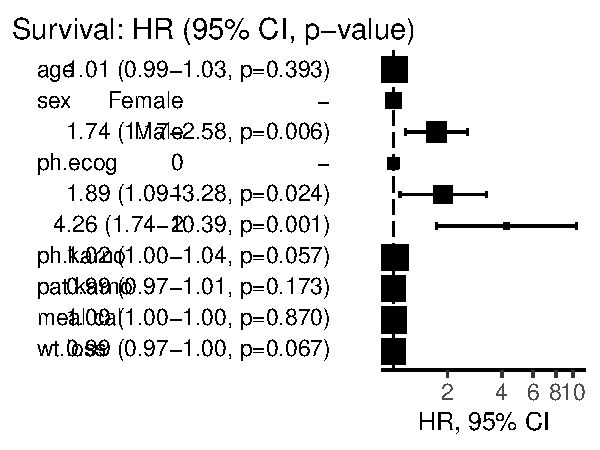
\includegraphics{final_project_files/figure-latex/unnamed-chunk-8-1.pdf}

\hypertarget{non-parametric-estimation}{%
\subsection{3 Non-parametric
Estimation}\label{non-parametric-estimation}}

\hypertarget{life-table}{%
\subsubsection{3.1 Life-table}\label{life-table}}

\begin{Shaded}
\begin{Highlighting}[]
\NormalTok{life\_table }\OtherTok{=}\NormalTok{ biostat3}\SpecialCharTok{::}\FunctionTok{lifetab2}\NormalTok{(}\FunctionTok{Surv}\NormalTok{(time, status}\SpecialCharTok{==}\DecValTok{1}\NormalTok{) }\SpecialCharTok{\textasciitilde{}} \DecValTok{1}\NormalTok{, lung\_df, }\AttributeTok{breaks =} \FunctionTok{seq}\NormalTok{(}\DecValTok{0}\NormalTok{, }\DecValTok{1200}\NormalTok{, }\DecValTok{100}\NormalTok{))}

\NormalTok{life\_table }\SpecialCharTok{\%\textgreater{}\%}
\NormalTok{  knitr}\SpecialCharTok{::}\FunctionTok{kable}\NormalTok{(}\AttributeTok{caption =} \StringTok{"Life{-}table Estimate"}\NormalTok{,}
               \AttributeTok{digits =} \DecValTok{4}\NormalTok{)}
\end{Highlighting}
\end{Shaded}

\begin{longtable}[]{@{}
  >{\raggedright\arraybackslash}p{(\columnwidth - 24\tabcolsep) * \real{0.1064}}
  >{\raggedleft\arraybackslash}p{(\columnwidth - 24\tabcolsep) * \real{0.0745}}
  >{\raggedleft\arraybackslash}p{(\columnwidth - 24\tabcolsep) * \real{0.0638}}
  >{\raggedleft\arraybackslash}p{(\columnwidth - 24\tabcolsep) * \real{0.0638}}
  >{\raggedleft\arraybackslash}p{(\columnwidth - 24\tabcolsep) * \real{0.0638}}
  >{\raggedleft\arraybackslash}p{(\columnwidth - 24\tabcolsep) * \real{0.0638}}
  >{\raggedleft\arraybackslash}p{(\columnwidth - 24\tabcolsep) * \real{0.0745}}
  >{\raggedleft\arraybackslash}p{(\columnwidth - 24\tabcolsep) * \real{0.0745}}
  >{\raggedleft\arraybackslash}p{(\columnwidth - 24\tabcolsep) * \real{0.0745}}
  >{\raggedleft\arraybackslash}p{(\columnwidth - 24\tabcolsep) * \real{0.0745}}
  >{\raggedleft\arraybackslash}p{(\columnwidth - 24\tabcolsep) * \real{0.0851}}
  >{\raggedleft\arraybackslash}p{(\columnwidth - 24\tabcolsep) * \real{0.0745}}
  >{\raggedleft\arraybackslash}p{(\columnwidth - 24\tabcolsep) * \real{0.1064}}@{}}
\caption{Life-table Estimate}\tabularnewline
\toprule()
\begin{minipage}[b]{\linewidth}\raggedright
\end{minipage} & \begin{minipage}[b]{\linewidth}\raggedleft
tstart
\end{minipage} & \begin{minipage}[b]{\linewidth}\raggedleft
tstop
\end{minipage} & \begin{minipage}[b]{\linewidth}\raggedleft
nsubs
\end{minipage} & \begin{minipage}[b]{\linewidth}\raggedleft
nlost
\end{minipage} & \begin{minipage}[b]{\linewidth}\raggedleft
nrisk
\end{minipage} & \begin{minipage}[b]{\linewidth}\raggedleft
nevent
\end{minipage} & \begin{minipage}[b]{\linewidth}\raggedleft
surv
\end{minipage} & \begin{minipage}[b]{\linewidth}\raggedleft
pdf
\end{minipage} & \begin{minipage}[b]{\linewidth}\raggedleft
hazard
\end{minipage} & \begin{minipage}[b]{\linewidth}\raggedleft
se.surv
\end{minipage} & \begin{minipage}[b]{\linewidth}\raggedleft
se.pdf
\end{minipage} & \begin{minipage}[b]{\linewidth}\raggedleft
se.hazard
\end{minipage} \\
\midrule()
\endfirsthead
\toprule()
\begin{minipage}[b]{\linewidth}\raggedright
\end{minipage} & \begin{minipage}[b]{\linewidth}\raggedleft
tstart
\end{minipage} & \begin{minipage}[b]{\linewidth}\raggedleft
tstop
\end{minipage} & \begin{minipage}[b]{\linewidth}\raggedleft
nsubs
\end{minipage} & \begin{minipage}[b]{\linewidth}\raggedleft
nlost
\end{minipage} & \begin{minipage}[b]{\linewidth}\raggedleft
nrisk
\end{minipage} & \begin{minipage}[b]{\linewidth}\raggedleft
nevent
\end{minipage} & \begin{minipage}[b]{\linewidth}\raggedleft
surv
\end{minipage} & \begin{minipage}[b]{\linewidth}\raggedleft
pdf
\end{minipage} & \begin{minipage}[b]{\linewidth}\raggedleft
hazard
\end{minipage} & \begin{minipage}[b]{\linewidth}\raggedleft
se.surv
\end{minipage} & \begin{minipage}[b]{\linewidth}\raggedleft
se.pdf
\end{minipage} & \begin{minipage}[b]{\linewidth}\raggedleft
se.hazard
\end{minipage} \\
\midrule()
\endhead
0-100 & 0 & 100 & 228 & 1 & 227.5 & 31 & 1.0000 & 0.0014 & 0.0015 &
0.0000 & 2e-04 & 0.0003 \\
100-200 & 100 & 200 & 196 & 11 & 190.5 & 41 & 0.8637 & 0.0019 & 0.0024 &
0.0227 & 3e-04 & 0.0004 \\
200-300 & 200 & 300 & 144 & 23 & 132.5 & 29 & 0.6778 & 0.0015 & 0.0025 &
0.0313 & 3e-04 & 0.0005 \\
300-400 & 300 & 400 & 92 & 10 & 87.0 & 25 & 0.5295 & 0.0015 & 0.0034 &
0.0345 & 3e-04 & 0.0007 \\
400-500 & 400 & 500 & 57 & 4 & 55.0 & 12 & 0.3773 & 0.0008 & 0.0024 &
0.0356 & 2e-04 & 0.0007 \\
500-600 & 500 & 600 & 41 & 7 & 37.5 & 10 & 0.2950 & 0.0008 & 0.0031 &
0.0349 & 2e-04 & 0.0010 \\
600-700 & 600 & 700 & 24 & 0 & 24.0 & 8 & 0.2163 & 0.0007 & 0.0040 &
0.0333 & 2e-04 & 0.0014 \\
700-800 & 700 & 800 & 16 & 1 & 15.5 & 7 & 0.1442 & 0.0007 & 0.0058 &
0.0304 & 2e-04 & 0.0021 \\
800-900 & 800 & 900 & 8 & 3 & 6.5 & 2 & 0.0791 & 0.0002 & 0.0036 &
0.0247 & 2e-04 & 0.0025 \\
900-1000 & 900 & 1000 & 3 & 1 & 2.5 & 0 & 0.0548 & 0.0000 & 0.0000 &
0.0223 & NaN & NaN \\
1000-1100 & 1000 & 1100 & 2 & 2 & 1.0 & 0 & 0.0548 & 0.0000 & 0.0000 &
0.0223 & NaN & NaN \\
1100-1200 & 1100 & 1200 & 0 & 0 & 0.0 & 0 & 0.0548 & NaN & NaN & 0.0223
& NaN & NaN \\
1200-Inf & 1200 & Inf & 0 & 0 & 0.0 & 0 & NaN & NA & NA & NaN & NA &
NA \\
\bottomrule()
\end{longtable}

\hypertarget{kaplan-meier-method}{%
\subsubsection{3.2 Kaplan-Meier method}\label{kaplan-meier-method}}

\begin{Shaded}
\begin{Highlighting}[]
\CommentTok{\# Find the number of days a person was alive before they died.}
\NormalTok{km\_dead }\OtherTok{\textless{}{-}} \FunctionTok{with}\NormalTok{(lung\_df, }\FunctionTok{Surv}\NormalTok{(time, status))}

\NormalTok{km\_dead }\OtherTok{\textless{}{-}} \FunctionTok{survfit}\NormalTok{(}\FunctionTok{Surv}\NormalTok{(time, status}\SpecialCharTok{==}\DecValTok{1}\NormalTok{) }\SpecialCharTok{\textasciitilde{}} \DecValTok{1}\NormalTok{, }\AttributeTok{data=}\NormalTok{lung\_df)}

\CommentTok{\# K{-}M plot}
\NormalTok{km\_dead }\SpecialCharTok{\%\textgreater{}\%} \FunctionTok{autoplot}\NormalTok{() }\SpecialCharTok{+} \FunctionTok{labs}\NormalTok{(}\AttributeTok{title=}\StringTok{"Kaplan{-}Meier Survival Cure with Confidence Interval"}\NormalTok{, }
                              \AttributeTok{x=}\StringTok{"Time (Days)"}\NormalTok{, }
                              \AttributeTok{y=}\StringTok{"Survival Probability S(t)"}\NormalTok{)}
\end{Highlighting}
\end{Shaded}

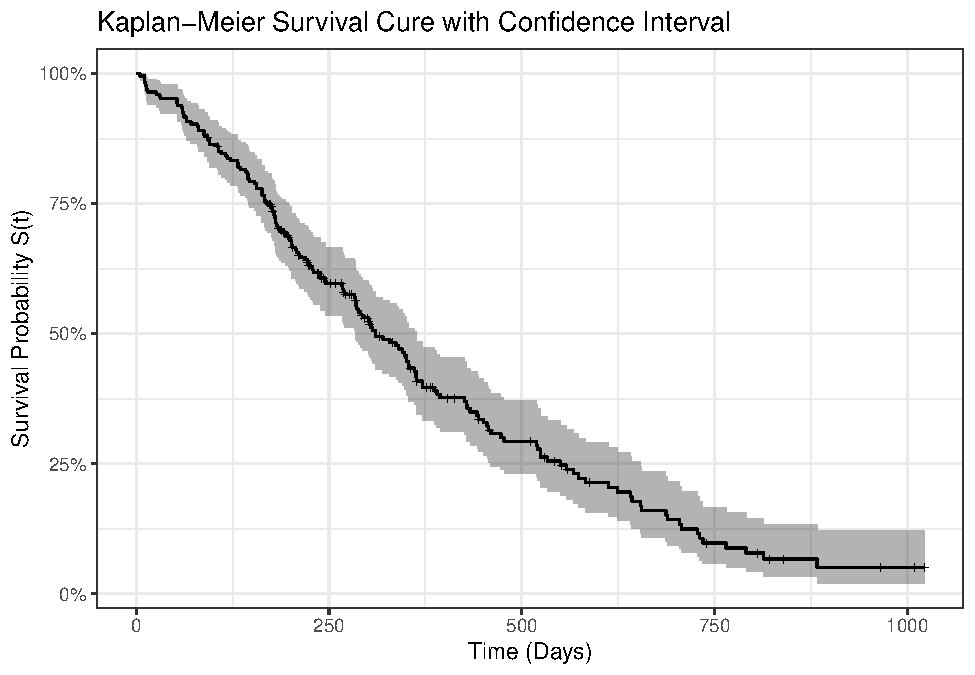
\includegraphics{final_project_files/figure-latex/unnamed-chunk-10-1.pdf}

\begin{Shaded}
\begin{Highlighting}[]
\CommentTok{\# Median survival time}
\FunctionTok{summary}\NormalTok{(km\_dead)}
\end{Highlighting}
\end{Shaded}

\begin{verbatim}
## Call: survfit(formula = Surv(time, status == 1) ~ 1, data = lung_df)
## 
##  time n.risk n.event survival std.err lower 95% CI upper 95% CI
##     5    228       1   0.9956 0.00438       0.9871        1.000
##    11    227       3   0.9825 0.00869       0.9656        1.000
##    12    224       1   0.9781 0.00970       0.9592        0.997
##    13    223       2   0.9693 0.01142       0.9472        0.992
##    15    221       1   0.9649 0.01219       0.9413        0.989
##    26    220       1   0.9605 0.01290       0.9356        0.986
##    30    219       1   0.9561 0.01356       0.9299        0.983
##    31    218       1   0.9518 0.01419       0.9243        0.980
##    53    217       2   0.9430 0.01536       0.9134        0.974
##    54    215       1   0.9386 0.01590       0.9079        0.970
##    59    214       1   0.9342 0.01642       0.9026        0.967
##    60    213       2   0.9254 0.01740       0.8920        0.960
##    61    211       1   0.9211 0.01786       0.8867        0.957
##    62    210       1   0.9167 0.01830       0.8815        0.953
##    65    209       2   0.9079 0.01915       0.8711        0.946
##    71    207       1   0.9035 0.01955       0.8660        0.943
##    79    206       1   0.8991 0.01995       0.8609        0.939
##    81    205       2   0.8904 0.02069       0.8507        0.932
##    88    203       2   0.8816 0.02140       0.8406        0.925
##    92    201       1   0.8772 0.02174       0.8356        0.921
##    93    199       1   0.8728 0.02207       0.8306        0.917
##    95    198       2   0.8640 0.02271       0.8206        0.910
##   105    196       1   0.8596 0.02302       0.8156        0.906
##   107    194       2   0.8507 0.02362       0.8056        0.898
##   110    192       1   0.8463 0.02391       0.8007        0.894
##   116    191       1   0.8418 0.02419       0.7957        0.891
##   118    190       1   0.8374 0.02446       0.7908        0.887
##   122    189       1   0.8330 0.02473       0.7859        0.883
##   131    188       1   0.8285 0.02500       0.7810        0.879
##   132    187       2   0.8197 0.02550       0.7712        0.871
##   135    185       1   0.8153 0.02575       0.7663        0.867
##   142    184       1   0.8108 0.02598       0.7615        0.863
##   144    183       1   0.8064 0.02622       0.7566        0.859
##   145    182       2   0.7975 0.02667       0.7469        0.852
##   147    180       1   0.7931 0.02688       0.7421        0.848
##   153    179       1   0.7887 0.02710       0.7373        0.844
##   156    178       2   0.7798 0.02751       0.7277        0.836
##   163    176       3   0.7665 0.02809       0.7134        0.824
##   166    173       2   0.7577 0.02845       0.7039        0.816
##   167    171       1   0.7532 0.02863       0.6991        0.811
##   170    170       1   0.7488 0.02880       0.6944        0.807
##   175    167       1   0.7443 0.02898       0.6896        0.803
##   176    165       1   0.7398 0.02915       0.6848        0.799
##   177    164       1   0.7353 0.02932       0.6800        0.795
##   179    162       2   0.7262 0.02965       0.6704        0.787
##   180    160       1   0.7217 0.02981       0.6655        0.783
##   181    159       2   0.7126 0.03012       0.6559        0.774
##   182    157       1   0.7081 0.03027       0.6511        0.770
##   183    156       1   0.7035 0.03041       0.6464        0.766
##   186    154       1   0.6989 0.03056       0.6416        0.761
##   189    152       1   0.6943 0.03070       0.6367        0.757
##   194    149       1   0.6897 0.03085       0.6318        0.753
##   197    147       1   0.6850 0.03099       0.6269        0.749
##   199    145       1   0.6803 0.03113       0.6219        0.744
##   201    144       2   0.6708 0.03141       0.6120        0.735
##   202    142       1   0.6661 0.03154       0.6071        0.731
##   207    139       1   0.6613 0.03168       0.6020        0.726
##   208    138       1   0.6565 0.03181       0.5970        0.722
##   210    137       1   0.6517 0.03194       0.5920        0.717
##   212    135       1   0.6469 0.03206       0.5870        0.713
##   218    134       1   0.6421 0.03218       0.5820        0.708
##   222    132       1   0.6372 0.03231       0.5769        0.704
##   223    130       1   0.6323 0.03243       0.5718        0.699
##   226    126       1   0.6273 0.03256       0.5666        0.694
##   229    125       1   0.6223 0.03268       0.5614        0.690
##   230    124       1   0.6172 0.03280       0.5562        0.685
##   239    121       2   0.6070 0.03304       0.5456        0.675
##   245    117       1   0.6019 0.03316       0.5402        0.670
##   246    116       1   0.5967 0.03328       0.5349        0.666
##   267    112       1   0.5913 0.03341       0.5294        0.661
##   268    111       1   0.5860 0.03353       0.5239        0.656
##   269    110       1   0.5807 0.03364       0.5184        0.651
##   270    108       1   0.5753 0.03376       0.5128        0.645
##   283    104       1   0.5698 0.03388       0.5071        0.640
##   284    103       1   0.5642 0.03400       0.5014        0.635
##   285    101       2   0.5531 0.03424       0.4899        0.624
##   286     99       1   0.5475 0.03434       0.4841        0.619
##   288     98       1   0.5419 0.03444       0.4784        0.614
##   291     97       1   0.5363 0.03454       0.4727        0.608
##   293     94       1   0.5306 0.03464       0.4669        0.603
##   301     91       1   0.5248 0.03475       0.4609        0.597
##   303     89       1   0.5189 0.03485       0.4549        0.592
##   305     87       1   0.5129 0.03496       0.4488        0.586
##   306     86       1   0.5070 0.03506       0.4427        0.581
##   310     85       2   0.4950 0.03523       0.4306        0.569
##   320     82       1   0.4890 0.03532       0.4244        0.563
##   329     81       1   0.4830 0.03539       0.4183        0.558
##   337     79       1   0.4768 0.03547       0.4121        0.552
##   340     78       1   0.4707 0.03554       0.4060        0.546
##   345     77       1   0.4646 0.03560       0.3998        0.540
##   348     76       1   0.4585 0.03565       0.3937        0.534
##   350     75       1   0.4524 0.03569       0.3876        0.528
##   351     74       1   0.4463 0.03573       0.3815        0.522
##   353     73       2   0.4340 0.03578       0.3693        0.510
##   361     70       1   0.4278 0.03581       0.3631        0.504
##   363     69       2   0.4154 0.03583       0.3508        0.492
##   364     67       1   0.4092 0.03582       0.3447        0.486
##   371     65       2   0.3966 0.03581       0.3323        0.473
##   387     60       1   0.3900 0.03582       0.3258        0.467
##   390     59       1   0.3834 0.03582       0.3193        0.460
##   394     58       1   0.3768 0.03580       0.3128        0.454
##   426     55       1   0.3700 0.03580       0.3060        0.447
##   428     54       1   0.3631 0.03579       0.2993        0.440
##   429     53       1   0.3563 0.03576       0.2926        0.434
##   433     52       1   0.3494 0.03573       0.2860        0.427
##   442     51       1   0.3426 0.03568       0.2793        0.420
##   444     50       1   0.3357 0.03561       0.2727        0.413
##   450     48       1   0.3287 0.03555       0.2659        0.406
##   455     47       1   0.3217 0.03548       0.2592        0.399
##   457     46       1   0.3147 0.03539       0.2525        0.392
##   460     44       1   0.3076 0.03530       0.2456        0.385
##   473     43       1   0.3004 0.03520       0.2388        0.378
##   477     42       1   0.2933 0.03508       0.2320        0.371
##   519     39       1   0.2857 0.03498       0.2248        0.363
##   520     38       1   0.2782 0.03485       0.2177        0.356
##   524     37       2   0.2632 0.03455       0.2035        0.340
##   533     34       1   0.2554 0.03439       0.1962        0.333
##   550     32       1   0.2475 0.03423       0.1887        0.325
##   558     30       1   0.2392 0.03407       0.1810        0.316
##   567     28       1   0.2307 0.03391       0.1729        0.308
##   574     27       1   0.2221 0.03371       0.1650        0.299
##   583     26       1   0.2136 0.03348       0.1571        0.290
##   613     24       1   0.2047 0.03325       0.1489        0.281
##   624     23       1   0.1958 0.03297       0.1407        0.272
##   641     22       1   0.1869 0.03265       0.1327        0.263
##   643     21       1   0.1780 0.03229       0.1247        0.254
##   654     20       1   0.1691 0.03188       0.1169        0.245
##   655     19       1   0.1602 0.03142       0.1091        0.235
##   687     18       1   0.1513 0.03090       0.1014        0.226
##   689     17       1   0.1424 0.03034       0.0938        0.216
##   705     16       1   0.1335 0.02972       0.0863        0.207
##   707     15       1   0.1246 0.02904       0.0789        0.197
##   728     14       1   0.1157 0.02830       0.0716        0.187
##   731     13       1   0.1068 0.02749       0.0645        0.177
##   735     12       1   0.0979 0.02660       0.0575        0.167
##   765     10       1   0.0881 0.02568       0.0498        0.156
##   791      9       1   0.0783 0.02462       0.0423        0.145
##   814      7       1   0.0671 0.02351       0.0338        0.133
##   883      4       1   0.0503 0.02285       0.0207        0.123
\end{verbatim}

\begin{Shaded}
\begin{Highlighting}[]
\FunctionTok{summary}\NormalTok{(km\_dead, }\AttributeTok{times =} \FunctionTok{c}\NormalTok{(}\DecValTok{300}\NormalTok{,}\DecValTok{305}\NormalTok{,}\DecValTok{310}\NormalTok{,}\DecValTok{315}\NormalTok{))}
\end{Highlighting}
\end{Shaded}

\begin{verbatim}
## Call: survfit(formula = Surv(time, status == 1) ~ 1, data = lung_df)
## 
##  time n.risk n.event survival std.err lower 95% CI upper 95% CI
##   300     92     101    0.531  0.0346        0.467        0.603
##   305     87       3    0.513  0.0350        0.449        0.586
##   310     85       3    0.495  0.0352        0.431        0.569
##   315     83       0    0.495  0.0352        0.431        0.569
\end{verbatim}

The median survival time is 310 days.

\begin{Shaded}
\begin{Highlighting}[]
\CommentTok{\# cumulative density with a confidence interval}
\FunctionTok{cuminc}\NormalTok{(}\FunctionTok{Surv}\NormalTok{(time, status) }\SpecialCharTok{\textasciitilde{}} \DecValTok{1}\NormalTok{, }\AttributeTok{data =}\NormalTok{ lung\_df) }\SpecialCharTok{\%\textgreater{}\%} 
  \FunctionTok{ggcuminc}\NormalTok{() }\SpecialCharTok{+} 
  \FunctionTok{labs}\NormalTok{(}
    \AttributeTok{x =} \StringTok{"Time (Days)"}
\NormalTok{  ) }\SpecialCharTok{+} 
  \FunctionTok{add\_confidence\_interval}\NormalTok{() }
\end{Highlighting}
\end{Shaded}

\begin{verbatim}
## Plotting outcome "1".
\end{verbatim}

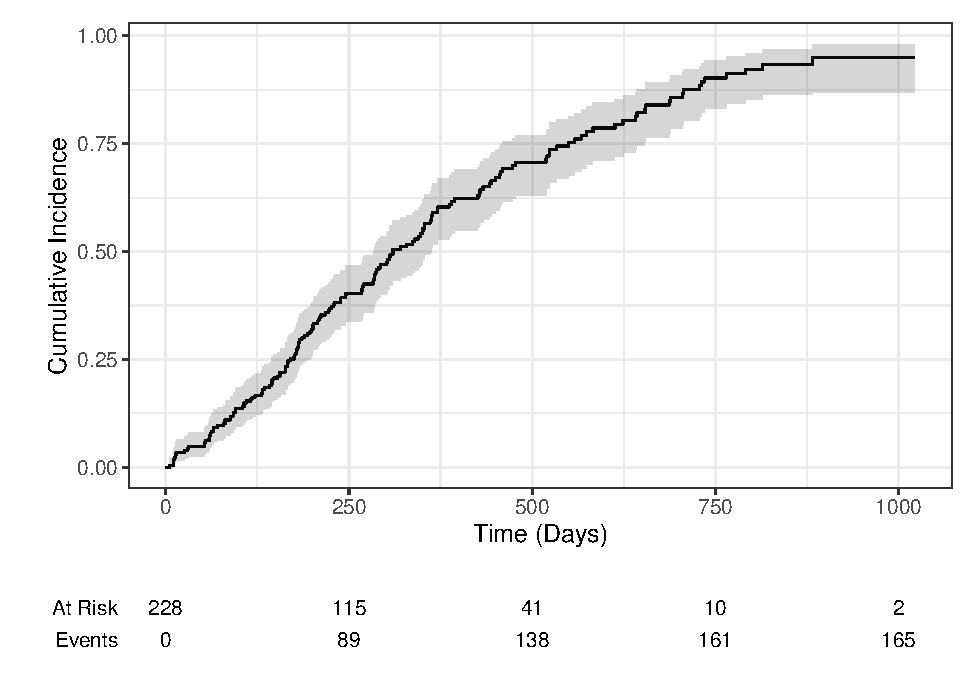
\includegraphics{final_project_files/figure-latex/unnamed-chunk-11-1.pdf}
As the number of survival days increase, the probability of a person
dying decreases.

\hypertarget{nelson-aalen-method}{%
\subsubsection{3.3 Nelson-Aalen method}\label{nelson-aalen-method}}

\hypertarget{overall-nelson-aalen-estimator}{%
\subsubsection{3.3.1 Overall Nelson-Aalen
Estimator}\label{overall-nelson-aalen-estimator}}

\begin{Shaded}
\begin{Highlighting}[]
\NormalTok{nelsonaalen }\OtherTok{=} \ControlFlowTok{function}\NormalTok{(data, timevar, statusvar) \{}
  \ControlFlowTok{if}\NormalTok{ (}\SpecialCharTok{!}\FunctionTok{is.data.frame}\NormalTok{(data)) \{}
    \FunctionTok{stop}\NormalTok{(}\StringTok{"Data must be a data frame"}\NormalTok{)}
\NormalTok{  \}}
\NormalTok{  timevar }\OtherTok{\textless{}{-}} \FunctionTok{as.character}\NormalTok{(}\FunctionTok{substitute}\NormalTok{(timevar))}
\NormalTok{  statusvar }\OtherTok{\textless{}{-}} \FunctionTok{as.character}\NormalTok{(}\FunctionTok{substitute}\NormalTok{(statusvar))}
\NormalTok{  time }\OtherTok{\textless{}{-}}\NormalTok{ data[, timevar, drop }\OtherTok{=} \ConstantTok{TRUE}\NormalTok{]}
\NormalTok{  status }\OtherTok{\textless{}{-}}\NormalTok{ data[, statusvar, drop }\OtherTok{=} \ConstantTok{TRUE}\NormalTok{]}

\NormalTok{  hazard }\OtherTok{\textless{}{-}}\NormalTok{ survival}\SpecialCharTok{::}\FunctionTok{basehaz}\NormalTok{(survival}\SpecialCharTok{::}\FunctionTok{coxph}\NormalTok{(survival}\SpecialCharTok{::}\FunctionTok{Surv}\NormalTok{(time, status}\SpecialCharTok{==}\DecValTok{1}\NormalTok{) }\SpecialCharTok{\textasciitilde{}} \DecValTok{1}\NormalTok{))}
\NormalTok{  idx }\OtherTok{\textless{}{-}} \FunctionTok{match}\NormalTok{(time, hazard[, }\StringTok{"time"}\NormalTok{])}
\NormalTok{  hazard[idx, }\StringTok{"hazard"}\NormalTok{]}
\NormalTok{\}}

\NormalTok{hazard }\OtherTok{=} \FunctionTok{nelsonaalen}\NormalTok{(lung\_df, time, status)}
\CommentTok{\# plot(x = lung\_df$time, main="Cumulative Probability for Event of Interest (Death)", y = hazard, ylab = "Cumulative Probability of subject\textquotesingle{}s death", xlab = "Number of Days") }


\NormalTok{lung\_df\_2 }\OtherTok{=}\NormalTok{ lung\_df }\SpecialCharTok{\%\textgreater{}\%} 
  \FunctionTok{mutate}\NormalTok{(}\AttributeTok{hazard =} \FunctionTok{nelsonaalen}\NormalTok{(lung\_df, time, status))}

\FunctionTok{ggplot}\NormalTok{(}\AttributeTok{data =}\NormalTok{ lung\_df\_2, }\FunctionTok{aes}\NormalTok{(}\AttributeTok{x =}\NormalTok{ time, }\AttributeTok{y =}\NormalTok{ hazard)) }\SpecialCharTok{+} 
  \FunctionTok{geom\_point}\NormalTok{(}\AttributeTok{alpha =}\NormalTok{ .}\DecValTok{3}\NormalTok{) }\SpecialCharTok{+}
  \FunctionTok{geom\_line}\NormalTok{(}\AttributeTok{colour =} \StringTok{"blue"}\NormalTok{) }\SpecialCharTok{+} 
  \FunctionTok{theme}\NormalTok{(}\AttributeTok{legend.position =} \StringTok{"bottom"}\NormalTok{) }\SpecialCharTok{+}
  \FunctionTok{labs}\NormalTok{(}
    \AttributeTok{title =} \StringTok{"Cumulative Hazard Rate for Event of Interest (Death)"}\NormalTok{,}
    \AttributeTok{x =} \StringTok{"Time (Days)"}\NormalTok{,}
    \AttributeTok{y =} \StringTok{"Cumulative Hazard Rate of Subject\textquotesingle{}s Death"}
\NormalTok{  )}
\end{Highlighting}
\end{Shaded}

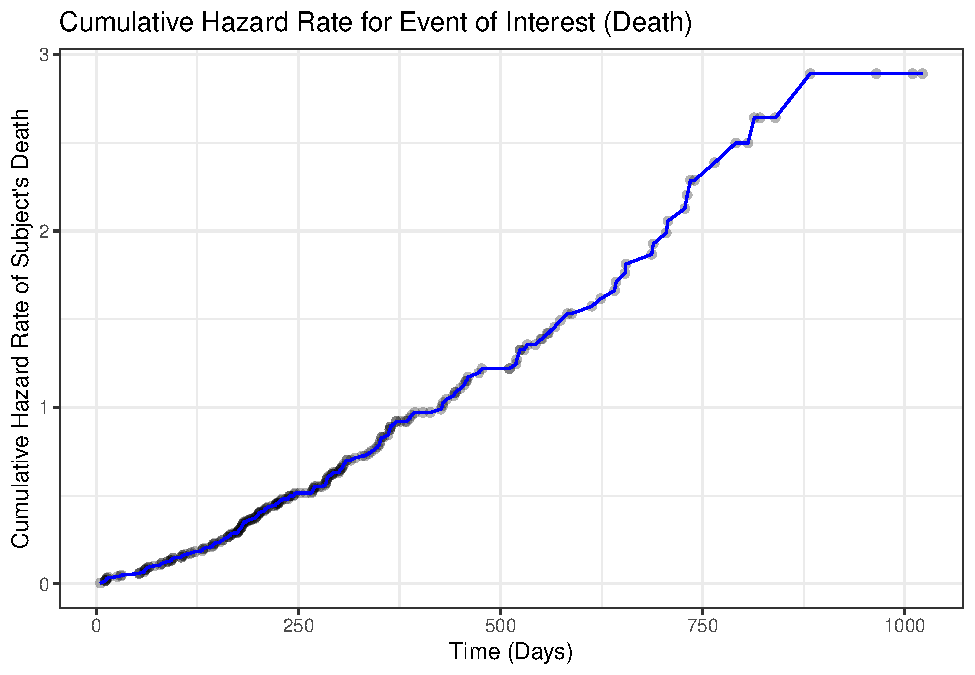
\includegraphics{final_project_files/figure-latex/unnamed-chunk-12-1.pdf}

\hypertarget{fleming-harrington-estimator}{%
\subsubsection{3.3.2 Fleming-Harrington
Estimator}\label{fleming-harrington-estimator}}

Once the H(t) of Nelson-Aalen hazard estimator is obtained,
Fleming-Harrington estimator for survival function can be obtained.

\begin{Shaded}
\begin{Highlighting}[]
\FunctionTok{survfit}\NormalTok{(}\FunctionTok{Surv}\NormalTok{(time, status}\SpecialCharTok{==}\DecValTok{1}\NormalTok{) }\SpecialCharTok{\textasciitilde{}} \DecValTok{1}\NormalTok{, lung\_df, }\AttributeTok{stype =} \DecValTok{1}\NormalTok{, }\AttributeTok{ctype =} \DecValTok{2}\NormalTok{)}
\end{Highlighting}
\end{Shaded}

\begin{verbatim}
## Call: survfit(formula = Surv(time, status == 1) ~ 1, data = lung_df, 
##     stype = 1, ctype = 2)
## 
##        n events median 0.95LCL 0.95UCL
## [1,] 228    165    310     285     363
\end{verbatim}

Fleming-Harrington estimator for median survival is 310, which is equal
to K-M estimator.

\hypertarget{hypothesis-testing}{%
\subsection{4 Hypothesis testing}\label{hypothesis-testing}}

In this section, we will make comparison of the different groups of the
attributes to identify the prognostic factors using the Kaplan-Meier
Curve and conduct log-rank test.

\hypertarget{univariate}{%
\subsubsection{4.1 Univariate}\label{univariate}}

We plan to combine ecog=3 with ecog=2 since there was only one subject
with ecog=3

\begin{Shaded}
\begin{Highlighting}[]
\NormalTok{lung\_df\_e }\OtherTok{=}\NormalTok{ lung\_df }\SpecialCharTok{\%\textgreater{}\%}
  \FunctionTok{mutate}\NormalTok{(}\AttributeTok{ph.ecog.n =} \FunctionTok{case\_when}\NormalTok{(ph.ecog }\SpecialCharTok{==} \DecValTok{0} \SpecialCharTok{\textasciitilde{}} \DecValTok{0}\NormalTok{,}
\NormalTok{                               ph.ecog }\SpecialCharTok{==} \DecValTok{1} \SpecialCharTok{\textasciitilde{}} \DecValTok{1}\NormalTok{,}
\NormalTok{                               ph.ecog }\SpecialCharTok{==} \DecValTok{2} \SpecialCharTok{\textasciitilde{}} \DecValTok{2}\NormalTok{,}
\NormalTok{                               ph.ecog }\SpecialCharTok{==} \DecValTok{3} \SpecialCharTok{\textasciitilde{}} \DecValTok{2}\NormalTok{)) }\SpecialCharTok{\%\textgreater{}\%}
  \FunctionTok{mutate}\NormalTok{(}\AttributeTok{ph.ecog.n =} \FunctionTok{as.factor}\NormalTok{(ph.ecog.n))}
\end{Highlighting}
\end{Shaded}

\hypertarget{sex}{%
\subsubsection{4.1.1 Sex}\label{sex}}

\begin{Shaded}
\begin{Highlighting}[]
\NormalTok{splots }\OtherTok{\textless{}{-}} \FunctionTok{list}\NormalTok{()}

\CommentTok{\# fit}
\NormalTok{lung\_sex }\OtherTok{=}\NormalTok{ lung\_df }\SpecialCharTok{\%\textgreater{}\%}
  \FunctionTok{drop\_na}\NormalTok{(sex) }\SpecialCharTok{\%\textgreater{}\%}
  \FunctionTok{mutate}\NormalTok{(}\AttributeTok{Sex =} \FunctionTok{case\_when}\NormalTok{(sex }\SpecialCharTok{==} \DecValTok{1} \SpecialCharTok{\textasciitilde{}} \StringTok{"Male"}\NormalTok{,}
\NormalTok{                         sex }\SpecialCharTok{==} \DecValTok{2} \SpecialCharTok{\textasciitilde{}} \StringTok{"Female"}\NormalTok{)) }

\NormalTok{fit\_sex }\OtherTok{=} \FunctionTok{survfit}\NormalTok{(}\FunctionTok{Surv}\NormalTok{(time, status}\SpecialCharTok{==}\DecValTok{1}\NormalTok{) }\SpecialCharTok{\textasciitilde{}}\NormalTok{ Sex, }\AttributeTok{data =}\NormalTok{ lung\_sex) }
\FunctionTok{summary}\NormalTok{(fit\_sex)}\SpecialCharTok{$}\NormalTok{table}
\end{Highlighting}
\end{Shaded}

\begin{verbatim}
##            records n.max n.start events    rmean se(rmean) median 0.95LCL
## Sex=Female      90    90      90     53 460.6473  34.68985    426     348
## Sex=Male       138   138     138    112 326.0841  22.91156    270     212
##            0.95UCL
## Sex=Female     550
## Sex=Male       310
\end{verbatim}

\begin{Shaded}
\begin{Highlighting}[]
\CommentTok{\# visualization}
\NormalTok{splots[[}\DecValTok{1}\NormalTok{]] }\OtherTok{=} \FunctionTok{ggsurvplot}\NormalTok{(fit\_sex,}
                         \AttributeTok{pval =} \ConstantTok{TRUE}\NormalTok{, }\AttributeTok{conf.int =} \ConstantTok{TRUE}\NormalTok{,}
                         \AttributeTok{surv.median.line =} \StringTok{"hv"}\NormalTok{, }\CommentTok{\# Specify median survival}
                         \AttributeTok{ggtheme =} \FunctionTok{theme\_bw}\NormalTok{(), }\CommentTok{\# Change ggplot2 theme}
                         \AttributeTok{legend =} \StringTok{"bottom"}\NormalTok{, }
                         \AttributeTok{legend.title =} \StringTok{"Sex"}\NormalTok{,}
                         \AttributeTok{legend.lab =} \FunctionTok{c}\NormalTok{(}\StringTok{"Female"}\NormalTok{, }\StringTok{"Male"}\NormalTok{))}

\CommentTok{\# log{-}rank test}
\NormalTok{diff\_sex }\OtherTok{=} \FunctionTok{survdiff}\NormalTok{(}\FunctionTok{Surv}\NormalTok{(time, status}\SpecialCharTok{==}\DecValTok{1}\NormalTok{) }\SpecialCharTok{\textasciitilde{}}\NormalTok{ Sex, }\AttributeTok{data =}\NormalTok{ lung\_sex) }
\NormalTok{diff\_sex}
\end{Highlighting}
\end{Shaded}

\begin{verbatim}
## Call:
## survdiff(formula = Surv(time, status == 1) ~ Sex, data = lung_sex)
## 
##              N Observed Expected (O-E)^2/E (O-E)^2/V
## Sex=Female  90       53     73.4      5.68      10.3
## Sex=Male   138      112     91.6      4.55      10.3
## 
##  Chisq= 10.3  on 1 degrees of freedom, p= 0.001
\end{verbatim}

\hypertarget{age}{%
\subsubsection{4.1.2 Age}\label{age}}

\begin{Shaded}
\begin{Highlighting}[]
\CommentTok{\# fit}
\NormalTok{lung\_age }\OtherTok{=}\NormalTok{ lung\_df }\SpecialCharTok{\%\textgreater{}\%}
  \FunctionTok{drop\_na}\NormalTok{(age) }\SpecialCharTok{\%\textgreater{}\%}
  \FunctionTok{mutate}\NormalTok{(}\AttributeTok{Age =} \FunctionTok{case\_when}\NormalTok{(age }\SpecialCharTok{\textgreater{}} \DecValTok{70} \SpecialCharTok{\textasciitilde{}} \StringTok{"\textgreater{} 70"}\NormalTok{,}
\NormalTok{                         age }\SpecialCharTok{\textless{}=} \DecValTok{70} \SpecialCharTok{\textasciitilde{}} \StringTok{"\textless{}= 70"}\NormalTok{)) }

\NormalTok{fit\_age }\OtherTok{=} \FunctionTok{survfit}\NormalTok{(}\FunctionTok{Surv}\NormalTok{(time, status}\SpecialCharTok{==}\DecValTok{1}\NormalTok{) }\SpecialCharTok{\textasciitilde{}}\NormalTok{ Age, }\AttributeTok{data =}\NormalTok{ lung\_age)}
\FunctionTok{summary}\NormalTok{(fit\_age)}\SpecialCharTok{$}\NormalTok{table}
\end{Highlighting}
\end{Shaded}

\begin{verbatim}
##           records n.max n.start events    rmean se(rmean) median 0.95LCL
## Age=<= 70     182   182     182    127 397.2120  22.40235    345     291
## Age=> 70       46    46      46     38 301.4505  39.31644    283     201
##           0.95UCL
## Age=<= 70     429
## Age=> 70      353
\end{verbatim}

\begin{Shaded}
\begin{Highlighting}[]
\CommentTok{\# visualization}
\NormalTok{splots[[}\DecValTok{2}\NormalTok{]] }\OtherTok{=} \FunctionTok{ggsurvplot}\NormalTok{(fit\_age,}
                         \AttributeTok{pval =} \ConstantTok{TRUE}\NormalTok{, }\AttributeTok{conf.int =} \ConstantTok{TRUE}\NormalTok{,}
                         \AttributeTok{surv.median.line =} \StringTok{"hv"}\NormalTok{, }
                         \AttributeTok{ggtheme =} \FunctionTok{theme\_bw}\NormalTok{(), }
                         \AttributeTok{legend =} \StringTok{"bottom"}\NormalTok{, }
                         \AttributeTok{legend.title =} \StringTok{"Age"}\NormalTok{,}
                         \AttributeTok{legend.lab =} \FunctionTok{c}\NormalTok{(}\StringTok{"\textless{}= 70"}\NormalTok{, }\StringTok{"\textgreater{} 70"}\NormalTok{))}

\CommentTok{\# log{-}rank test}
\NormalTok{diff\_age }\OtherTok{=} \FunctionTok{survdiff}\NormalTok{(}\FunctionTok{Surv}\NormalTok{(time, status}\SpecialCharTok{==}\DecValTok{1}\NormalTok{) }\SpecialCharTok{\textasciitilde{}}\NormalTok{ Age, }\AttributeTok{data =}\NormalTok{ lung\_age) }
\NormalTok{diff\_age}
\end{Highlighting}
\end{Shaded}

\begin{verbatim}
## Call:
## survdiff(formula = Surv(time, status == 1) ~ Age, data = lung_age)
## 
##             N Observed Expected (O-E)^2/E (O-E)^2/V
## Age=<= 70 182      127    137.3     0.773      4.64
## Age=> 70   46       38     27.7     3.829      4.64
## 
##  Chisq= 4.6  on 1 degrees of freedom, p= 0.03
\end{verbatim}

\hypertarget{ecog-performance-score}{%
\subsubsection{4.1.3 ECOG performance
score}\label{ecog-performance-score}}

\begin{Shaded}
\begin{Highlighting}[]
\CommentTok{\# fit}
\NormalTok{lung\_ecog }\OtherTok{=}\NormalTok{ lung\_df\_e }\SpecialCharTok{\%\textgreater{}\%}
  \FunctionTok{drop\_na}\NormalTok{(ph.ecog) }\SpecialCharTok{\%\textgreater{}\%}
  \FunctionTok{mutate}\NormalTok{(}\AttributeTok{ph.ecog =} \FunctionTok{as.factor}\NormalTok{(ph.ecog)) }

\NormalTok{fit\_ecog }\OtherTok{=} \FunctionTok{survfit}\NormalTok{(}\FunctionTok{Surv}\NormalTok{(time, status}\SpecialCharTok{==}\DecValTok{1}\NormalTok{) }\SpecialCharTok{\textasciitilde{}}\NormalTok{ ph.ecog.n, }\AttributeTok{data =}\NormalTok{ lung\_ecog)}
\FunctionTok{summary}\NormalTok{(fit\_ecog)}\SpecialCharTok{$}\NormalTok{table}
\end{Highlighting}
\end{Shaded}

\begin{verbatim}
##             records n.max n.start events    rmean se(rmean) median 0.95LCL
## ph.ecog.n=0      63    63      63     37 465.3131  42.88835    394     348
## ph.ecog.n=1     113   113     113     82 384.8410  27.28943    306     268
## ph.ecog.n=2      51    51      51     45 255.7636  30.74032    183     153
##             0.95UCL
## ph.ecog.n=0     574
## ph.ecog.n=1     429
## ph.ecog.n=2     288
\end{verbatim}

\begin{Shaded}
\begin{Highlighting}[]
\CommentTok{\# visualization}
\NormalTok{splots[[}\DecValTok{3}\NormalTok{]] }\OtherTok{=} \FunctionTok{ggsurvplot}\NormalTok{(fit\_ecog,}
                         \AttributeTok{pval =} \ConstantTok{TRUE}\NormalTok{, }\AttributeTok{conf.int =} \ConstantTok{TRUE}\NormalTok{,}
                         \AttributeTok{surv.median.line =} \StringTok{"hv"}\NormalTok{, }
                         \AttributeTok{ggtheme =} \FunctionTok{theme\_bw}\NormalTok{(), }
                         \AttributeTok{legend =} \StringTok{"bottom"}\NormalTok{, }
                         \AttributeTok{legend.title =} \StringTok{"ECOG Performance Score"}\NormalTok{,}
                         \AttributeTok{legend.lab =} \FunctionTok{c}\NormalTok{(}\StringTok{"0"}\NormalTok{, }\StringTok{"1"}\NormalTok{, }\StringTok{"2"}\NormalTok{))}

\CommentTok{\# log{-}rank test}
\NormalTok{diff\_ecog }\OtherTok{=} \FunctionTok{survdiff}\NormalTok{(}\FunctionTok{Surv}\NormalTok{(time, status}\SpecialCharTok{==}\DecValTok{1}\NormalTok{) }\SpecialCharTok{\textasciitilde{}}\NormalTok{ ph.ecog, }\AttributeTok{data =}\NormalTok{ lung\_ecog) }
\NormalTok{diff\_ecog}
\end{Highlighting}
\end{Shaded}

\begin{verbatim}
## Call:
## survdiff(formula = Surv(time, status == 1) ~ ph.ecog, data = lung_ecog)
## 
##             N Observed Expected (O-E)^2/E (O-E)^2/V
## ph.ecog=0  63       37   54.153    5.4331    8.2119
## ph.ecog=1 113       82   83.528    0.0279    0.0573
## ph.ecog=2  50       44   26.147   12.1893   14.6491
## ph.ecog=3   1        1    0.172    3.9733    4.0040
## 
##  Chisq= 22  on 3 degrees of freedom, p= 7e-05
\end{verbatim}

\hypertarget{karnofsky-performance-score-rated-by-physician}{%
\subsubsection{4.1.4 Karnofsky performance score rated by
physician}\label{karnofsky-performance-score-rated-by-physician}}

\begin{Shaded}
\begin{Highlighting}[]
\CommentTok{\# fit}
\NormalTok{lung\_phkarno }\OtherTok{=}\NormalTok{ lung\_df }\SpecialCharTok{\%\textgreater{}\%}
  \FunctionTok{drop\_na}\NormalTok{(ph.karno) }\SpecialCharTok{\%\textgreater{}\%}
  \FunctionTok{mutate}\NormalTok{(}\AttributeTok{ph.karno =} \FunctionTok{case\_when}\NormalTok{(ph.karno }\SpecialCharTok{\textgreater{}} \DecValTok{80} \SpecialCharTok{\textasciitilde{}} \StringTok{"\textgreater{} 80"}\NormalTok{,}
\NormalTok{                         ph.karno }\SpecialCharTok{\textless{}=} \DecValTok{80} \SpecialCharTok{\textasciitilde{}} \StringTok{"\textless{}= 80"}\NormalTok{)) }

\NormalTok{fit\_phkarno }\OtherTok{=} \FunctionTok{survfit}\NormalTok{(}\FunctionTok{Surv}\NormalTok{(time, status}\SpecialCharTok{==}\DecValTok{1}\NormalTok{) }\SpecialCharTok{\textasciitilde{}}\NormalTok{ ph.karno, }\AttributeTok{data=}\NormalTok{lung\_phkarno)}
\FunctionTok{summary}\NormalTok{(fit\_phkarno)}\SpecialCharTok{$}\NormalTok{table}
\end{Highlighting}
\end{Shaded}

\begin{verbatim}
##                records n.max n.start events    rmean se(rmean) median 0.95LCL
## ph.karno=<= 80     124   124     124     97 329.3139  24.55953    239     202
## ph.karno=> 80      103   103     103     67 431.8672  30.51428    394     340
##                0.95UCL
## ph.karno=<= 80     305
## ph.karno=> 80      473
\end{verbatim}

\begin{Shaded}
\begin{Highlighting}[]
\CommentTok{\# visualization}
\NormalTok{splots[[}\DecValTok{4}\NormalTok{]] }\OtherTok{=} \FunctionTok{ggsurvplot}\NormalTok{(fit\_phkarno,}
                         \AttributeTok{pval =} \ConstantTok{TRUE}\NormalTok{, }\AttributeTok{conf.int =} \ConstantTok{TRUE}\NormalTok{,}
                         \AttributeTok{surv.median.line =} \StringTok{"hv"}\NormalTok{, }
                         \AttributeTok{ggtheme =} \FunctionTok{theme\_bw}\NormalTok{(), }
                         \AttributeTok{legend =} \StringTok{"bottom"}\NormalTok{, }
                         \AttributeTok{legend.title =} \StringTok{"Karnofsky Score by Physician"}\NormalTok{,}
                         \AttributeTok{legend.lab =} \FunctionTok{c}\NormalTok{(}\StringTok{"\textless{}= 80"}\NormalTok{, }\StringTok{"\textgreater{} 80"}\NormalTok{))}

\CommentTok{\# log{-}rank test}
\NormalTok{diff\_phkarno }\OtherTok{=} \FunctionTok{survdiff}\NormalTok{(}\FunctionTok{Surv}\NormalTok{(time, status}\SpecialCharTok{==}\DecValTok{1}\NormalTok{) }\SpecialCharTok{\textasciitilde{}}\NormalTok{ ph.karno, }\AttributeTok{data =}\NormalTok{ lung\_phkarno) }
\NormalTok{diff\_phkarno}
\end{Highlighting}
\end{Shaded}

\begin{verbatim}
## Call:
## survdiff(formula = Surv(time, status == 1) ~ ph.karno, data = lung_phkarno)
## 
##                  N Observed Expected (O-E)^2/E (O-E)^2/V
## ph.karno=<= 80 124       97     79.2      4.01      7.84
## ph.karno=> 80  103       67     84.8      3.74      7.84
## 
##  Chisq= 7.8  on 1 degrees of freedom, p= 0.005
\end{verbatim}

\hypertarget{karnofsky-performance-score-as-rated-by-patient}{%
\subsubsection{4.1.5 Karnofsky performance score as rated by
patient}\label{karnofsky-performance-score-as-rated-by-patient}}

\begin{Shaded}
\begin{Highlighting}[]
\CommentTok{\# fit}
\NormalTok{lung\_patkarno }\OtherTok{=}\NormalTok{ lung\_df }\SpecialCharTok{\%\textgreater{}\%}
  \FunctionTok{drop\_na}\NormalTok{(pat.karno) }\SpecialCharTok{\%\textgreater{}\%}
  \FunctionTok{mutate}\NormalTok{(}\AttributeTok{pat.karno =} \FunctionTok{case\_when}\NormalTok{(pat.karno }\SpecialCharTok{\textgreater{}} \DecValTok{80} \SpecialCharTok{\textasciitilde{}} \StringTok{"\textgreater{} 80"}\NormalTok{,}
\NormalTok{                         pat.karno }\SpecialCharTok{\textless{}=} \DecValTok{80} \SpecialCharTok{\textasciitilde{}} \StringTok{"\textless{}= 80"}\NormalTok{)) }

\NormalTok{fit\_patkarno }\OtherTok{=} \FunctionTok{survfit}\NormalTok{(}\FunctionTok{Surv}\NormalTok{(time, status}\SpecialCharTok{==}\DecValTok{1}\NormalTok{) }\SpecialCharTok{\textasciitilde{}}\NormalTok{ pat.karno, }\AttributeTok{data=}\NormalTok{lung\_patkarno)}
\FunctionTok{summary}\NormalTok{(fit\_patkarno)}\SpecialCharTok{$}\NormalTok{table}
\end{Highlighting}
\end{Shaded}

\begin{verbatim}
##                 records n.max n.start events    rmean se(rmean) median 0.95LCL
## pat.karno=<= 80     130   130     130    103 336.1857  24.34974    239     202
## pat.karno=> 80       95    95      95     59 440.3736  32.69968    371     320
##                 0.95UCL
## pat.karno=<= 80     348
## pat.karno=> 80      477
\end{verbatim}

\begin{Shaded}
\begin{Highlighting}[]
\CommentTok{\# visualization}
\NormalTok{splots[[}\DecValTok{5}\NormalTok{]] }\OtherTok{=} \FunctionTok{ggsurvplot}\NormalTok{(fit\_patkarno,}
                         \AttributeTok{pval =} \ConstantTok{TRUE}\NormalTok{, }\AttributeTok{conf.int =} \ConstantTok{TRUE}\NormalTok{,}
                         \AttributeTok{surv.median.line =} \StringTok{"hv"}\NormalTok{, }
                         \AttributeTok{ggtheme =} \FunctionTok{theme\_bw}\NormalTok{(), }
                         \AttributeTok{legend =} \StringTok{"bottom"}\NormalTok{, }
                         \AttributeTok{legend.title =} \StringTok{"Karnofsky Score by Patient"}\NormalTok{,}
                         \AttributeTok{legend.lab =} \FunctionTok{c}\NormalTok{(}\StringTok{"\textless{}= 80"}\NormalTok{, }\StringTok{"\textgreater{} 80"}\NormalTok{))}

\CommentTok{\# log{-}rank test}
\NormalTok{diff\_patkarno }\OtherTok{=} \FunctionTok{survdiff}\NormalTok{(}\FunctionTok{Surv}\NormalTok{(time, status}\SpecialCharTok{==}\DecValTok{1}\NormalTok{) }\SpecialCharTok{\textasciitilde{}}\NormalTok{ pat.karno, }\AttributeTok{data =}\NormalTok{ lung\_patkarno) }
\NormalTok{diff\_patkarno}
\end{Highlighting}
\end{Shaded}

\begin{verbatim}
## Call:
## survdiff(formula = Surv(time, status == 1) ~ pat.karno, data = lung_patkarno)
## 
##                   N Observed Expected (O-E)^2/E (O-E)^2/V
## pat.karno=<= 80 130      103     85.5      3.60      7.69
## pat.karno=> 80   95       59     76.5      4.02      7.69
## 
##  Chisq= 7.7  on 1 degrees of freedom, p= 0.006
\end{verbatim}

\hypertarget{calories-consumed-at-meals}{%
\subsubsection{4.1.6 Calories consumed at
meals}\label{calories-consumed-at-meals}}

\begin{Shaded}
\begin{Highlighting}[]
\CommentTok{\# fit}
\NormalTok{avg\_meal\_cal }\OtherTok{=} \FunctionTok{mean}\NormalTok{(}\FunctionTok{as.numeric}\NormalTok{(lung\_df}\SpecialCharTok{$}\NormalTok{meal.cal), }\AttributeTok{na.rm =} \ConstantTok{TRUE}\NormalTok{)}

\NormalTok{lung\_meal\_cal }\OtherTok{=}\NormalTok{ lung\_df }\SpecialCharTok{\%\textgreater{}\%}
  \FunctionTok{drop\_na}\NormalTok{(meal.cal) }\SpecialCharTok{\%\textgreater{}\%}
  \FunctionTok{mutate}\NormalTok{(}\AttributeTok{meal.cal =} \FunctionTok{case\_when}\NormalTok{(meal.cal }\SpecialCharTok{\textgreater{}}\NormalTok{ avg\_meal\_cal }\SpecialCharTok{\textasciitilde{}} \StringTok{"\textgreater{} average"}\NormalTok{,}
\NormalTok{                         meal.cal }\SpecialCharTok{\textless{}=}\NormalTok{ avg\_meal\_cal }\SpecialCharTok{\textasciitilde{}} \StringTok{"\textless{}= average"}\NormalTok{)) }

\NormalTok{fit\_meal\_cal }\OtherTok{=} \FunctionTok{survfit}\NormalTok{(}\FunctionTok{Surv}\NormalTok{(time, status}\SpecialCharTok{==}\DecValTok{1}\NormalTok{) }\SpecialCharTok{\textasciitilde{}}\NormalTok{ meal.cal, }\AttributeTok{data =}\NormalTok{ lung\_meal\_cal)}
\FunctionTok{summary}\NormalTok{(fit\_meal\_cal)}\SpecialCharTok{$}\NormalTok{table}
\end{Highlighting}
\end{Shaded}

\begin{verbatim}
##                     records n.max n.start events    rmean se(rmean) median
## meal.cal=<= average      82    82      82     60 353.7694  37.04280    285
## meal.cal=> average       99    99      99     74 383.4524  27.52114    348
##                     0.95LCL 0.95UCL
## meal.cal=<= average     212     351
## meal.cal=> average      285     450
\end{verbatim}

\begin{Shaded}
\begin{Highlighting}[]
\NormalTok{splots[[}\DecValTok{6}\NormalTok{]] }\OtherTok{=} \FunctionTok{ggsurvplot}\NormalTok{(fit\_meal\_cal, }
                         \AttributeTok{pval =} \ConstantTok{TRUE}\NormalTok{, }\AttributeTok{conf.int =} \ConstantTok{TRUE}\NormalTok{,}
                         \AttributeTok{surv.median.line =} \StringTok{"hv"}\NormalTok{, }
                         \AttributeTok{ggtheme =} \FunctionTok{theme\_bw}\NormalTok{(), }
                         \AttributeTok{legend =} \StringTok{"bottom"}\NormalTok{,}
                         \AttributeTok{legend.title =} \StringTok{"Calories Consumed at Meals"}\NormalTok{,}
                         \AttributeTok{legend.lab =} \FunctionTok{c}\NormalTok{(}\StringTok{"\textless{}= average"}\NormalTok{, }\StringTok{"\textgreater{} average"}\NormalTok{))}

\CommentTok{\# log{-}rank test}
\NormalTok{diff\_meal\_cal }\OtherTok{=} \FunctionTok{survdiff}\NormalTok{(}\FunctionTok{Surv}\NormalTok{(time, status}\SpecialCharTok{==}\DecValTok{1}\NormalTok{) }\SpecialCharTok{\textasciitilde{}}\NormalTok{ meal.cal, }\AttributeTok{data =}\NormalTok{ lung\_meal\_cal) }
\NormalTok{diff\_meal\_cal}
\end{Highlighting}
\end{Shaded}

\begin{verbatim}
## Call:
## survdiff(formula = Surv(time, status == 1) ~ meal.cal, data = lung_meal_cal)
## 
##                      N Observed Expected (O-E)^2/E (O-E)^2/V
## meal.cal=<= average 82       60     55.2     0.419     0.723
## meal.cal=> average  99       74     78.8     0.294     0.723
## 
##  Chisq= 0.7  on 1 degrees of freedom, p= 0.4
\end{verbatim}

\hypertarget{weight-loss}{%
\subsubsection{4.1.7 Weight loss}\label{weight-loss}}

\begin{Shaded}
\begin{Highlighting}[]
\CommentTok{\# fit}
\NormalTok{avg\_wt\_loss }\OtherTok{=} \FunctionTok{mean}\NormalTok{(}\FunctionTok{as.numeric}\NormalTok{(lung\_df}\SpecialCharTok{$}\NormalTok{wt.loss), }\AttributeTok{na.rm =} \ConstantTok{TRUE}\NormalTok{)}

\NormalTok{lung\_wt\_loss }\OtherTok{=}\NormalTok{ lung\_df }\SpecialCharTok{\%\textgreater{}\%}
  \FunctionTok{drop\_na}\NormalTok{(wt.loss) }\SpecialCharTok{\%\textgreater{}\%}
  \FunctionTok{mutate}\NormalTok{(}\AttributeTok{wt.loss =} \FunctionTok{case\_when}\NormalTok{(wt.loss }\SpecialCharTok{\textgreater{}}\NormalTok{ avg\_wt\_loss }\SpecialCharTok{\textasciitilde{}} \StringTok{"\textgreater{} average"}\NormalTok{,}
\NormalTok{                         wt.loss }\SpecialCharTok{\textless{}=}\NormalTok{ avg\_wt\_loss }\SpecialCharTok{\textasciitilde{}} \StringTok{"\textless{}= average"}\NormalTok{)) }

\NormalTok{fit\_wt\_loss }\OtherTok{\textless{}{-}} \FunctionTok{survfit}\NormalTok{(}\FunctionTok{Surv}\NormalTok{(time, status}\SpecialCharTok{==}\DecValTok{1}\NormalTok{) }\SpecialCharTok{\textasciitilde{}}\NormalTok{ wt.loss, }\AttributeTok{data =}\NormalTok{ lung\_wt\_loss)}
\FunctionTok{summary}\NormalTok{(fit\_wt\_loss)}\SpecialCharTok{$}\NormalTok{table}
\end{Highlighting}
\end{Shaded}

\begin{verbatim}
##                    records n.max n.start events    rmean se(rmean) median
## wt.loss=<= average     121   121     121     79 419.7671  28.90820    364
## wt.loss=> average       93    93      93     73 350.5749  28.34981    288
##                    0.95LCL 0.95UCL
## wt.loss=<= average     320     450
## wt.loss=> average      223     351
\end{verbatim}

\begin{Shaded}
\begin{Highlighting}[]
\CommentTok{\# visualization}
\NormalTok{splots[[}\DecValTok{7}\NormalTok{]] }\OtherTok{=} \FunctionTok{ggsurvplot}\NormalTok{(fit\_wt\_loss, }
                         \AttributeTok{pval =} \ConstantTok{TRUE}\NormalTok{, }\AttributeTok{conf.int =} \ConstantTok{TRUE}\NormalTok{,}
                         \AttributeTok{surv.median.line =} \StringTok{"hv"}\NormalTok{, }
                         \AttributeTok{ggtheme =} \FunctionTok{theme\_bw}\NormalTok{(), }
                         \AttributeTok{legend =} \StringTok{"bottom"}\NormalTok{,}
                         \AttributeTok{legend.title =} \StringTok{"Weight loss (Lbs)"}\NormalTok{,}
                         \AttributeTok{legend.lab =} \FunctionTok{c}\NormalTok{(}\StringTok{"\textless{}= average"}\NormalTok{, }\StringTok{"\textgreater{} average"}\NormalTok{))}

\CommentTok{\# log{-}rank test}
\NormalTok{diff\_wt\_loss }\OtherTok{=} \FunctionTok{survdiff}\NormalTok{(}\FunctionTok{Surv}\NormalTok{(time, status}\SpecialCharTok{==}\DecValTok{1}\NormalTok{) }\SpecialCharTok{\textasciitilde{}}\NormalTok{ wt.loss, }\AttributeTok{data =}\NormalTok{ lung\_wt\_loss) }
\NormalTok{diff\_wt\_loss}
\end{Highlighting}
\end{Shaded}

\begin{verbatim}
## Call:
## survdiff(formula = Surv(time, status == 1) ~ wt.loss, data = lung_wt_loss)
## 
##                      N Observed Expected (O-E)^2/E (O-E)^2/V
## wt.loss=<= average 121       79     89.7      1.27      3.12
## wt.loss=> average   93       73     62.3      1.82      3.12
## 
##  Chisq= 3.1  on 1 degrees of freedom, p= 0.08
\end{verbatim}

\begin{Shaded}
\begin{Highlighting}[]
\CommentTok{\# combine the plots}
\FunctionTok{arrange\_ggsurvplots}\NormalTok{(splots, }
                    \AttributeTok{print =} \ConstantTok{TRUE}\NormalTok{,}
                    \AttributeTok{title =} \StringTok{"Comparison of the Different Attribute Groups Using the Kaplan{-}Meier Curve"}\NormalTok{,}
                    \AttributeTok{ncol =} \DecValTok{2}\NormalTok{, }
                    \AttributeTok{nrow =} \DecValTok{4}\NormalTok{)}
\end{Highlighting}
\end{Shaded}

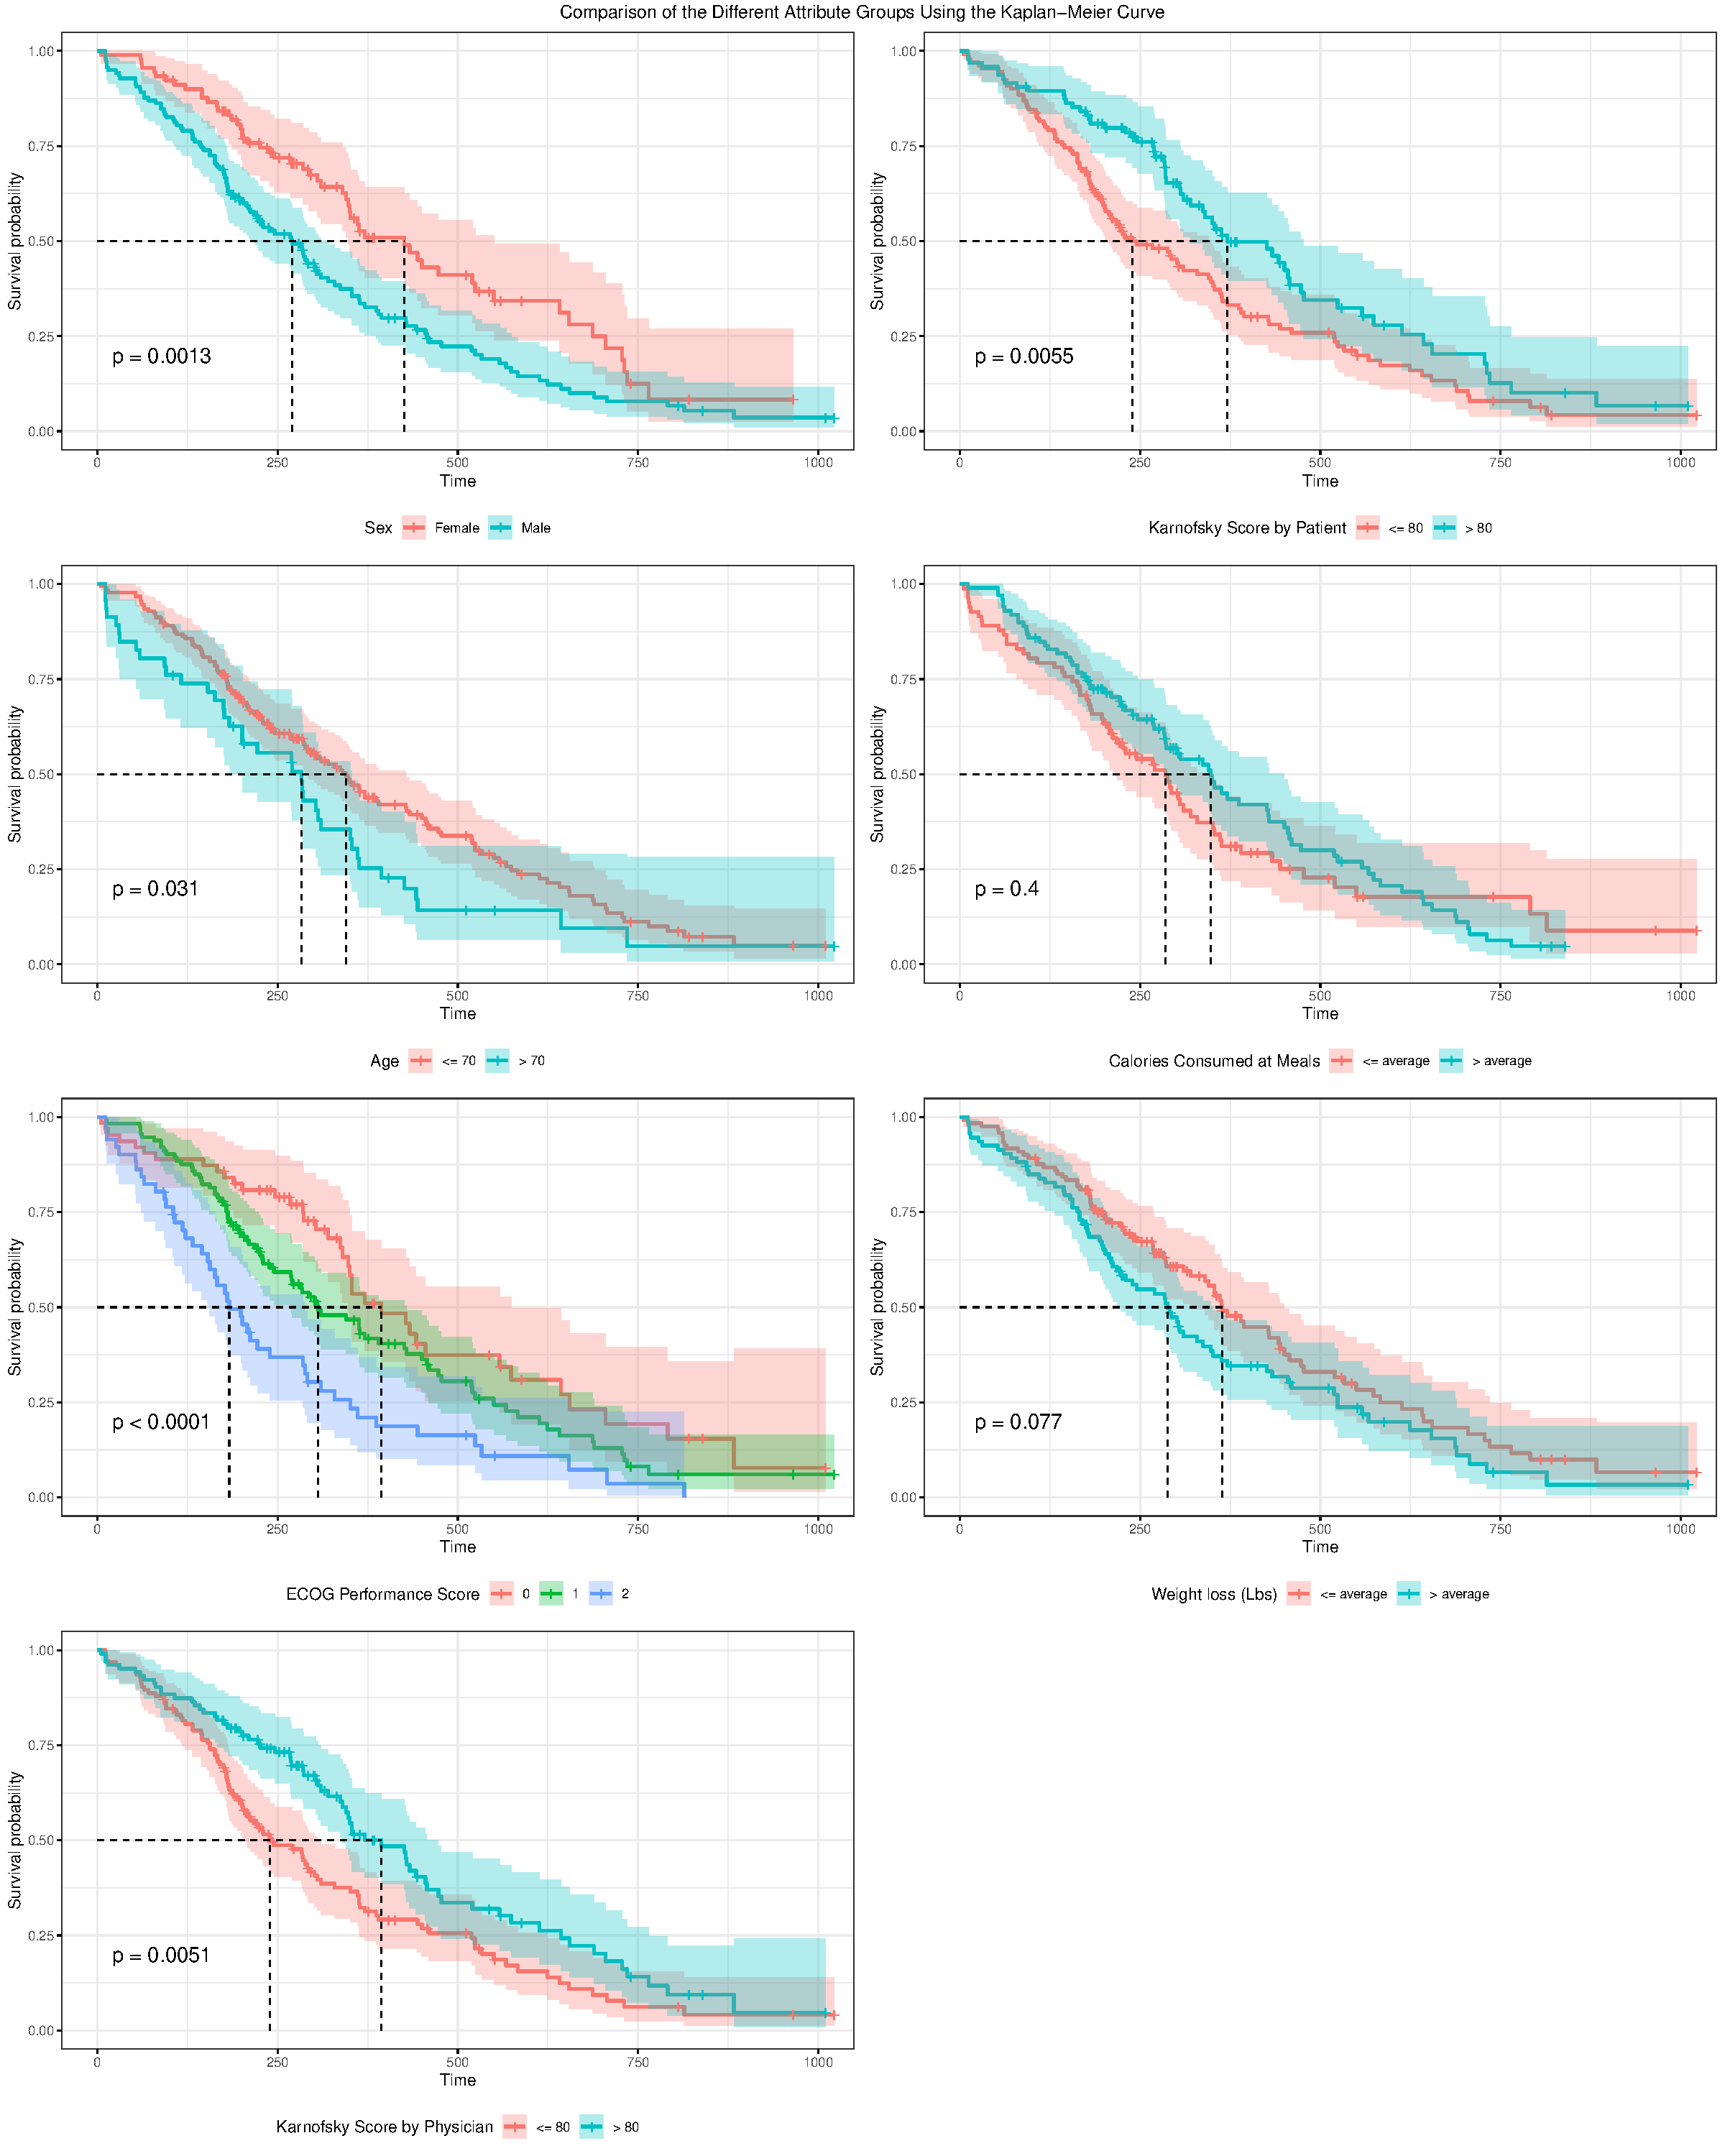
\includegraphics{final_project_files/figure-latex/unnamed-chunk-22-1.pdf}

Age, sex, ph.ecog, ph.karno, pat.karno can be identified as prognostic
factors.

\hypertarget{multivariate}{%
\subsubsection{4.2 Multivariate}\label{multivariate}}

\hypertarget{sex-ph.ecog}{%
\subsection{4.2.1 sex + ph.ecog}\label{sex-ph.ecog}}

\begin{Shaded}
\begin{Highlighting}[]
\CommentTok{\# fit}
\NormalTok{lung\_sex\_ecog }\OtherTok{=}\NormalTok{ lung\_df\_e }\SpecialCharTok{\%\textgreater{}\%}
  \FunctionTok{drop\_na}\NormalTok{(sex, ph.ecog.n) }\SpecialCharTok{\%\textgreater{}\%}
  \FunctionTok{mutate}\NormalTok{(}\AttributeTok{ph.ecog =} \FunctionTok{as.factor}\NormalTok{(ph.ecog)) }\SpecialCharTok{\%\textgreater{}\%}
  \FunctionTok{mutate}\NormalTok{(}\AttributeTok{Sex =} \FunctionTok{case\_when}\NormalTok{(sex }\SpecialCharTok{==} \DecValTok{1} \SpecialCharTok{\textasciitilde{}} \StringTok{"Male"}\NormalTok{,}
\NormalTok{                         sex }\SpecialCharTok{==} \DecValTok{2} \SpecialCharTok{\textasciitilde{}} \StringTok{"Female"}\NormalTok{)) }

\NormalTok{fit\_sex\_ecog }\OtherTok{=} \FunctionTok{survfit}\NormalTok{(}\FunctionTok{Surv}\NormalTok{(time, status}\SpecialCharTok{==}\DecValTok{1}\NormalTok{) }\SpecialCharTok{\textasciitilde{}}\NormalTok{ Sex }\SpecialCharTok{+}\NormalTok{ ph.ecog.n, }\AttributeTok{data =}\NormalTok{ lung\_sex\_ecog)}
\FunctionTok{summary}\NormalTok{(fit\_sex\_ecog)}\SpecialCharTok{$}\NormalTok{table}
\end{Highlighting}
\end{Shaded}

\begin{verbatim}
##                         records n.max n.start events    rmean se(rmean) median
## Sex=Female, ph.ecog.n=0      27    27      27      9 586.9179  95.23307  705.0
## Sex=Female, ph.ecog.n=1      42    42      42     28 475.3713  45.14073  450.0
## Sex=Female, ph.ecog.n=2      21    21      21     16 300.9587  44.61934  239.0
## Sex=Male, ph.ecog.n=0        36    36      36     28 415.5025  48.59025  353.0
## Sex=Male, ph.ecog.n=1        71    71      71     54 327.6528  31.77508  239.0
## Sex=Male, ph.ecog.n=2        30    30      30     29 222.4667  38.93727  164.5
##                         0.95LCL 0.95UCL
## Sex=Female, ph.ecog.n=0     350      NA
## Sex=Female, ph.ecog.n=1     345     687
## Sex=Female, ph.ecog.n=2     199     444
## Sex=Male, ph.ecog.n=0       303     558
## Sex=Male, ph.ecog.n=1       207     363
## Sex=Male, ph.ecog.n=2       105     288
\end{verbatim}

\begin{Shaded}
\begin{Highlighting}[]
\CommentTok{\# subset}
\CommentTok{\#fit\_sex\_ecog\_1 = survfit(Surv(time, status==1) \textasciitilde{} Sex + ph.ecog, data = subset(lung\_sex\_ecog, ph.ecog \%in\% c(0,1)))}
\CommentTok{\#summary(fit\_sex\_ecog\_1)$table}

\CommentTok{\# visualization}
\FunctionTok{ggsurvplot}\NormalTok{(fit\_sex\_ecog,}
           \AttributeTok{pval =} \ConstantTok{TRUE}\NormalTok{, }\AttributeTok{conf.int =} \ConstantTok{FALSE}\NormalTok{,}
           \AttributeTok{surv.median.line =} \StringTok{"hv"}\NormalTok{, }
           \AttributeTok{ggtheme =} \FunctionTok{theme\_bw}\NormalTok{(), }
           \AttributeTok{legend =} \StringTok{"bottom"}\NormalTok{)}
\end{Highlighting}
\end{Shaded}

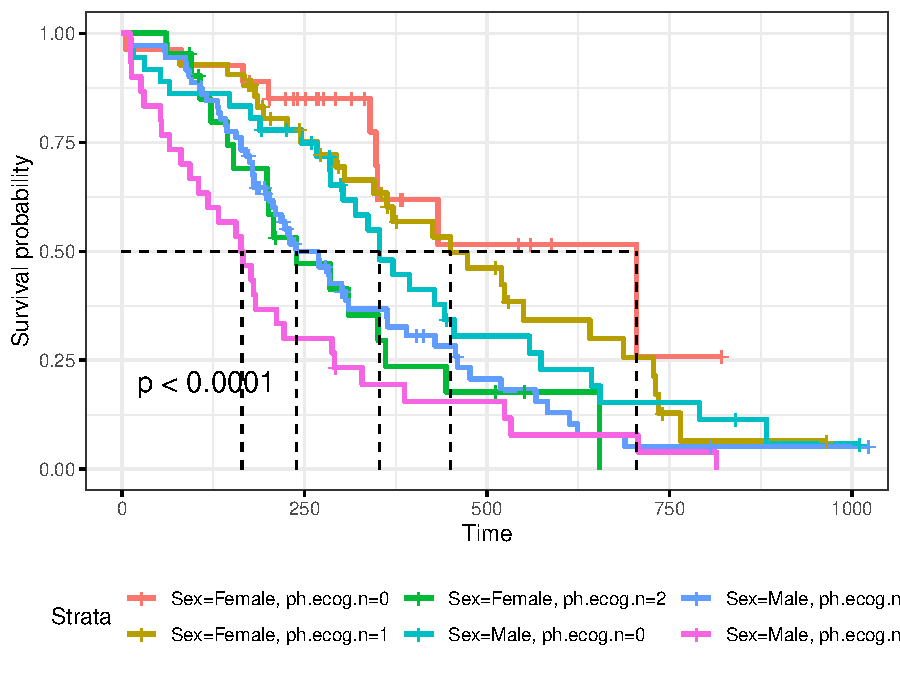
\includegraphics{final_project_files/figure-latex/unnamed-chunk-23-1.pdf}

\begin{Shaded}
\begin{Highlighting}[]
\CommentTok{\# ggsurvplot(fit\_sex\_ecog\_1,}
\CommentTok{\#          pval = TRUE, conf.int = FALSE,}
\CommentTok{\#          surv.median.line = "hv", }
\CommentTok{\#          ggtheme = theme\_bw(), }
\CommentTok{\#          legend = "bottom")}

\CommentTok{\# log{-}rank test}
\NormalTok{diff\_sex\_ecog }\OtherTok{=} \FunctionTok{survdiff}\NormalTok{(}\FunctionTok{Surv}\NormalTok{(time, status}\SpecialCharTok{==}\DecValTok{1}\NormalTok{) }\SpecialCharTok{\textasciitilde{}}\NormalTok{ Sex }\SpecialCharTok{+}\NormalTok{ ph.ecog.n, }\AttributeTok{data =}\NormalTok{ lung\_sex\_ecog) }
\NormalTok{diff\_sex\_ecog}
\end{Highlighting}
\end{Shaded}

\begin{verbatim}
## Call:
## survdiff(formula = Surv(time, status == 1) ~ Sex + ph.ecog.n, 
##     data = lung_sex_ecog)
## 
##                          N Observed Expected (O-E)^2/E (O-E)^2/V
## Sex=Female, ph.ecog.n=0 27        9     21.1     6.940     8.020
## Sex=Female, ph.ecog.n=1 42       28     40.2     3.707     4.999
## Sex=Female, ph.ecog.n=2 21       16     11.7     1.553     1.693
## Sex=Male, ph.ecog.n=0   36       28     33.1     0.772     0.986
## Sex=Male, ph.ecog.n=1   71       54     43.3     2.634     3.636
## Sex=Male, ph.ecog.n=2   30       29     14.6    14.236    15.740
## 
##  Chisq= 30.3  on 5 degrees of freedom, p= 1e-05
\end{verbatim}

We find that female with ecog = 1 may have a higher survival probability
than male with ecog = 0.

And then we explore more by SAS.

\begin{figure}
\centering
\includegraphics{plot/sex+ecog.jpg}
\caption{Survival Function between sex and ecog}
\end{figure}

\hypertarget{age-ph.ecog}{%
\subsection{4.2.2 age + ph.ecog}\label{age-ph.ecog}}

\begin{Shaded}
\begin{Highlighting}[]
\CommentTok{\# fit}
\NormalTok{lung\_age\_ecog }\OtherTok{=}\NormalTok{ lung\_df\_e }\SpecialCharTok{\%\textgreater{}\%}
  \FunctionTok{drop\_na}\NormalTok{(age, ph.ecog.n) }\SpecialCharTok{\%\textgreater{}\%}
  \FunctionTok{mutate}\NormalTok{(}\AttributeTok{Age =} \FunctionTok{case\_when}\NormalTok{(age }\SpecialCharTok{\textgreater{}} \DecValTok{70} \SpecialCharTok{\textasciitilde{}} \StringTok{"\textgreater{} 70"}\NormalTok{,}
\NormalTok{                         age }\SpecialCharTok{\textless{}=} \DecValTok{70} \SpecialCharTok{\textasciitilde{}} \StringTok{"\textless{}= 70"}\NormalTok{)) }

\NormalTok{fit\_age\_ecog }\OtherTok{=} \FunctionTok{survfit}\NormalTok{(}\FunctionTok{Surv}\NormalTok{(time, status}\SpecialCharTok{==}\DecValTok{1}\NormalTok{) }\SpecialCharTok{\textasciitilde{}}\NormalTok{ Age }\SpecialCharTok{+}\NormalTok{ ph.ecog.n, }\AttributeTok{data =}\NormalTok{ lung\_age\_ecog)}
\FunctionTok{summary}\NormalTok{(fit\_age\_ecog)}\SpecialCharTok{$}\NormalTok{table}
\end{Highlighting}
\end{Shaded}

\begin{verbatim}
##                        records n.max n.start events    rmean se(rmean) median
## Age=<= 70, ph.ecog.n=0      53    53      53     28 506.6747  49.90976    433
## Age=<= 70, ph.ecog.n=1      97    97      97     70 384.1550  29.10006    345
## Age=<= 70, ph.ecog.n=2      31    31      31     28 279.1563  39.24119    208
## Age=> 70, ph.ecog.n=0       10    10      10      9 298.1000  61.39223    303
## Age=> 70, ph.ecog.n=1       16    16      16     12 390.8731  73.72300    306
## Age=> 70, ph.ecog.n=2       20    20      20     17 257.0818  68.02154    163
##                        0.95LCL 0.95UCL
## Age=<= 70, ph.ecog.n=0     348     705
## Age=<= 70, ph.ecog.n=1     230     460
## Age=<= 70, ph.ecog.n=2     156     329
## Age=> 70, ph.ecog.n=0      176      NA
## Age=> 70, ph.ecog.n=1      270      NA
## Age=> 70, ph.ecog.n=2       93     361
\end{verbatim}

\begin{Shaded}
\begin{Highlighting}[]
\CommentTok{\# visualization}
\FunctionTok{ggsurvplot}\NormalTok{(fit\_age\_ecog,}
           \AttributeTok{pval =} \ConstantTok{TRUE}\NormalTok{, }\AttributeTok{conf.int =} \ConstantTok{FALSE}\NormalTok{,}
           \AttributeTok{surv.median.line =} \StringTok{"hv"}\NormalTok{, }
           \AttributeTok{ggtheme =} \FunctionTok{theme\_bw}\NormalTok{(), }
           \AttributeTok{legend =} \StringTok{"bottom"}\NormalTok{)}
\end{Highlighting}
\end{Shaded}

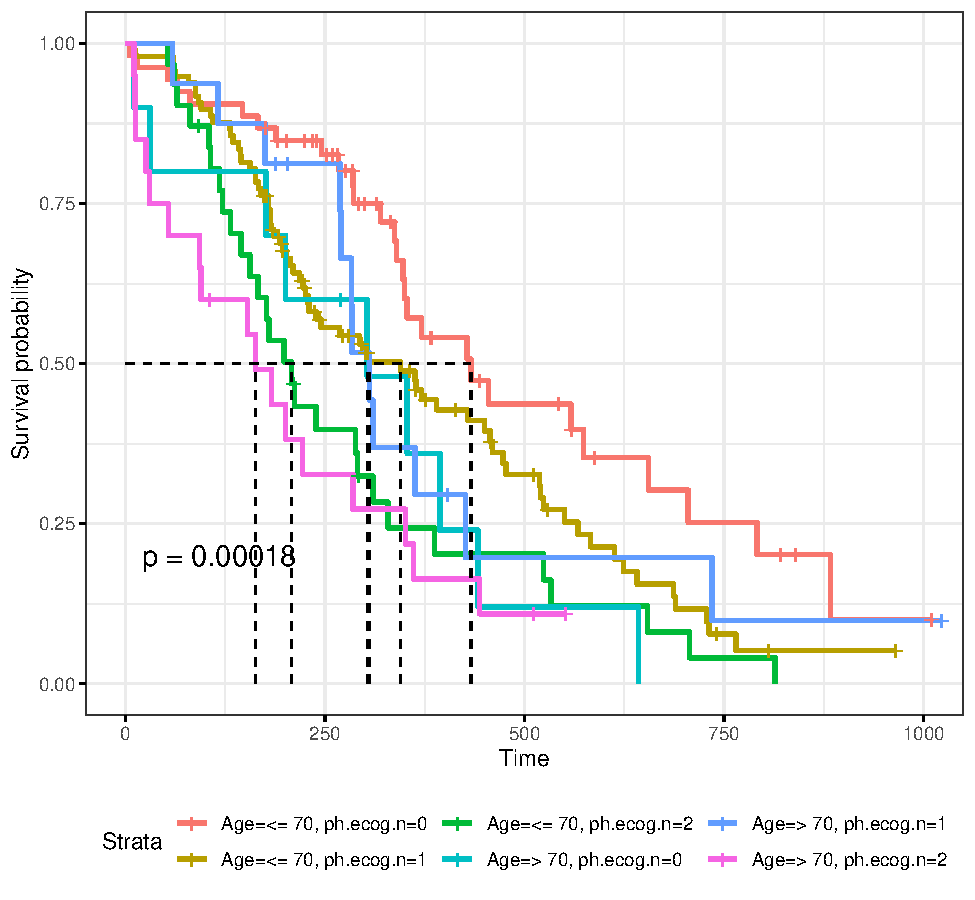
\includegraphics{final_project_files/figure-latex/unnamed-chunk-24-1.pdf}

\begin{Shaded}
\begin{Highlighting}[]
\CommentTok{\# log{-}rank test}
\NormalTok{diff\_age\_ecog }\OtherTok{=} \FunctionTok{survdiff}\NormalTok{(}\FunctionTok{Surv}\NormalTok{(time, status}\SpecialCharTok{==}\DecValTok{1}\NormalTok{) }\SpecialCharTok{\textasciitilde{}}\NormalTok{ Age }\SpecialCharTok{+}\NormalTok{ ph.ecog.n, }\AttributeTok{data =}\NormalTok{ lung\_age\_ecog) }
\NormalTok{diff\_age\_ecog}
\end{Highlighting}
\end{Shaded}

\begin{verbatim}
## Call:
## survdiff(formula = Surv(time, status == 1) ~ Age + ph.ecog.n, 
##     data = lung_age_ecog)
## 
##                         N Observed Expected (O-E)^2/E (O-E)^2/V
## Age=<= 70, ph.ecog.n=0 53       28    47.66   8.10776   11.6127
## Age=<= 70, ph.ecog.n=1 97       70    70.69   0.00683    0.0121
## Age=<= 70, ph.ecog.n=2 31       28    18.11   5.40377    6.1178
## Age=> 70, ph.ecog.n=0  10        9     6.50   0.96530    1.0129
## Age=> 70, ph.ecog.n=1  16       12    12.83   0.05403    0.0592
## Age=> 70, ph.ecog.n=2  20       17     8.21   9.40529   10.0304
## 
##  Chisq= 24.4  on 5 degrees of freedom, p= 2e-04
\end{verbatim}

\hypertarget{ph.karno-pat.karno}{%
\subsubsection{4.2.3 ph.karno + pat.karno}\label{ph.karno-pat.karno}}

\begin{Shaded}
\begin{Highlighting}[]
\CommentTok{\# fit}
\NormalTok{lung\_ph\_pat }\OtherTok{=}\NormalTok{ lung\_df }\SpecialCharTok{\%\textgreater{}\%}
  \FunctionTok{drop\_na}\NormalTok{(ph.karno, pat.karno) }\SpecialCharTok{\%\textgreater{}\%}
  \FunctionTok{mutate}\NormalTok{(}\AttributeTok{ph.karno =} \FunctionTok{case\_when}\NormalTok{(ph.karno }\SpecialCharTok{\textgreater{}} \DecValTok{80} \SpecialCharTok{\textasciitilde{}} \StringTok{"  \textgreater{} 80"}\NormalTok{,}
\NormalTok{                         ph.karno }\SpecialCharTok{\textless{}=} \DecValTok{80} \SpecialCharTok{\textasciitilde{}} \StringTok{"  \textless{}= 80"}\NormalTok{)) }\SpecialCharTok{\%\textgreater{}\%}
   \FunctionTok{mutate}\NormalTok{(}\AttributeTok{pat.karno =} \FunctionTok{case\_when}\NormalTok{(pat.karno }\SpecialCharTok{\textgreater{}} \DecValTok{80} \SpecialCharTok{\textasciitilde{}} \StringTok{"  \textgreater{} 80"}\NormalTok{,}
\NormalTok{                         ph.karno }\SpecialCharTok{\textless{}=} \DecValTok{80} \SpecialCharTok{\textasciitilde{}} \StringTok{"  \textless{}= 80"}\NormalTok{)) }

\NormalTok{fit\_ph\_pat }\OtherTok{=} \FunctionTok{survfit}\NormalTok{(}\FunctionTok{Surv}\NormalTok{(time, status}\SpecialCharTok{==}\DecValTok{1}\NormalTok{) }\SpecialCharTok{\textasciitilde{}}\NormalTok{ ph.karno }\SpecialCharTok{+}\NormalTok{ pat.karno, }\AttributeTok{data=}\NormalTok{lung\_ph\_pat)}
\FunctionTok{summary}\NormalTok{(fit\_ph\_pat)}\SpecialCharTok{$}\NormalTok{table}
\end{Highlighting}
\end{Shaded}

\begin{verbatim}
##                                     records n.max n.start events    rmean
## ph.karno=  <= 80, pat.karno=  <= 80      87    87      87     72 323.1235
## ph.karno=  <= 80, pat.karno=  > 80       35    35      35     23 366.4192
## ph.karno=  > 80, pat.karno=  <= 80       42    42      42     30 368.5197
## ph.karno=  > 80, pat.karno=  > 80        60    60      60     36 484.2746
##                                     se(rmean) median 0.95LCL 0.95UCL
## ph.karno=  <= 80, pat.karno=  <= 80  27.36178    229     194     351
## ph.karno=  <= 80, pat.karno=  > 80   60.00332    283     230     524
## ph.karno=  > 80, pat.karno=  <= 80   49.36250    303     210     429
## ph.karno=  > 80, pat.karno=  > 80    38.18366    455     353     613
\end{verbatim}

\begin{Shaded}
\begin{Highlighting}[]
\CommentTok{\# visualization}
\FunctionTok{ggsurvplot}\NormalTok{(fit\_ph\_pat,}
           \AttributeTok{pval =} \ConstantTok{TRUE}\NormalTok{, }\AttributeTok{conf.int =} \ConstantTok{FALSE}\NormalTok{,}
           \AttributeTok{surv.median.line =} \StringTok{"hv"}\NormalTok{, }
           \AttributeTok{ggtheme =} \FunctionTok{theme\_bw}\NormalTok{(), }
           \AttributeTok{legend =} \StringTok{"bottom"}\NormalTok{)}
\end{Highlighting}
\end{Shaded}

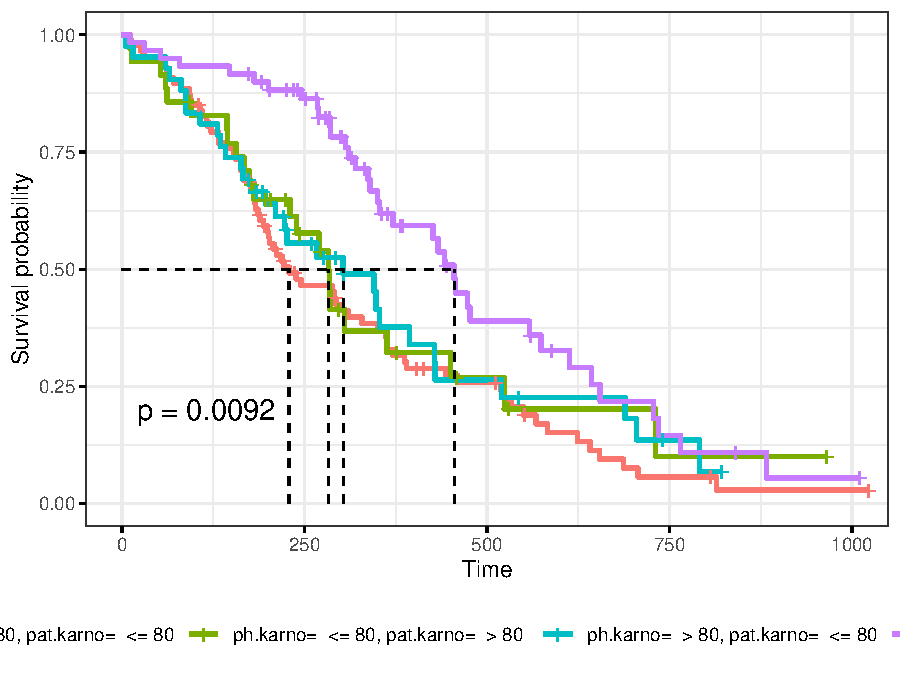
\includegraphics{final_project_files/figure-latex/unnamed-chunk-25-1.pdf}

\begin{Shaded}
\begin{Highlighting}[]
\CommentTok{\# log{-}rank test}
\NormalTok{diff\_ph\_pat }\OtherTok{=} \FunctionTok{survdiff}\NormalTok{(}\FunctionTok{Surv}\NormalTok{(time, status}\SpecialCharTok{==}\DecValTok{1}\NormalTok{) }\SpecialCharTok{\textasciitilde{}}\NormalTok{ ph.karno }\SpecialCharTok{+}\NormalTok{ pat.karno, }\AttributeTok{data =}\NormalTok{ lung\_ph\_pat) }
\NormalTok{diff\_ph\_pat}
\end{Highlighting}
\end{Shaded}

\begin{verbatim}
## Call:
## survdiff(formula = Surv(time, status == 1) ~ ph.karno + pat.karno, 
##     data = lung_ph_pat)
## 
##                                      N Observed Expected (O-E)^2/E (O-E)^2/V
## ph.karno=  <= 80, pat.karno=  <= 80 87       72     56.7     4.116     6.410
## ph.karno=  <= 80, pat.karno=  > 80  35       23     20.6     0.275     0.318
## ph.karno=  > 80, pat.karno=  <= 80  42       30     28.1     0.127     0.156
## ph.karno=  > 80, pat.karno=  > 80   60       36     55.6     6.883    10.636
## 
##  Chisq= 11.5  on 3 degrees of freedom, p= 0.009
\end{verbatim}

We find that ph.karno \(>\) 80 and pat.karno \(\le\) 80 may have a
higher survival probability than ph.karno \(\le\) 80 and pat.karno
\(>\), which means that physicians may predict better.

And then we explore more by SAS.

\begin{figure}
\centering
\includegraphics{plot/karno.jpg}
\caption{Survival Function between Karnofsky score rated by physician
and patient}
\end{figure}

\hypertarget{model-fitting-cox-model}{%
\subsection{5 Model Fitting (Cox Model)}\label{model-fitting-cox-model}}

\hypertarget{full-model}{%
\subsubsection{5.1 Full model}\label{full-model}}

\begin{Shaded}
\begin{Highlighting}[]
\NormalTok{lung\_mod }\OtherTok{=}\NormalTok{ lung\_df\_e }\SpecialCharTok{\%\textgreater{}\%}
  \FunctionTok{drop\_na}\NormalTok{()}

\CommentTok{\# full model}
\NormalTok{cox\_mod\_1 }\OtherTok{=} \FunctionTok{coxph}\NormalTok{(}\FunctionTok{Surv}\NormalTok{(time, status}\SpecialCharTok{==}\DecValTok{1}\NormalTok{) }\SpecialCharTok{\textasciitilde{}}\NormalTok{ sex }\SpecialCharTok{+}\NormalTok{ age }\SpecialCharTok{+}\NormalTok{ ph.ecog.n }\SpecialCharTok{+}\NormalTok{ ph.karno }\SpecialCharTok{+}\NormalTok{ pat.karno }\SpecialCharTok{+}\NormalTok{ meal.cal }\SpecialCharTok{+}\NormalTok{ wt.loss, }\AttributeTok{data =}\NormalTok{ lung\_mod)}
\FunctionTok{summary}\NormalTok{(cox\_mod\_1)}
\end{Highlighting}
\end{Shaded}

\begin{verbatim}
## Call:
## coxph(formula = Surv(time, status == 1) ~ sex + age + ph.ecog.n + 
##     ph.karno + pat.karno + meal.cal + wt.loss, data = lung_mod)
## 
##   n= 167, number of events= 120 
## 
##                  coef  exp(coef)   se(coef)      z Pr(>|z|)   
## sex2       -5.574e-01  5.727e-01  2.021e-01 -2.759  0.00580 **
## age         1.013e-02  1.010e+00  1.170e-02  0.866  0.38645   
## ph.ecog.n1  6.387e-01  1.894e+00  2.818e-01  2.266  0.02343 * 
## ph.ecog.n2  1.466e+00  4.332e+00  4.603e-01  3.184  0.00145 **
## ph.karno    2.140e-02  1.022e+00  1.125e-02  1.902  0.05717 . 
## pat.karno  -1.097e-02  9.891e-01  8.543e-03 -1.284  0.19901   
## meal.cal    3.704e-05  1.000e+00  2.586e-04  0.143  0.88608   
## wt.loss    -1.415e-02  9.859e-01  7.797e-03 -1.815  0.06947 . 
## ---
## Signif. codes:  0 '***' 0.001 '**' 0.01 '*' 0.05 '.' 0.1 ' ' 1
## 
##            exp(coef) exp(-coef) lower .95 upper .95
## sex2          0.5727     1.7461    0.3854     0.851
## age           1.0102     0.9899    0.9873     1.034
## ph.ecog.n1    1.8940     0.5280    1.0902     3.291
## ph.ecog.n2    4.3316     0.2309    1.7572    10.678
## ph.karno      1.0216     0.9788    0.9993     1.044
## pat.karno     0.9891     1.0110    0.9727     1.006
## meal.cal      1.0000     1.0000    0.9995     1.001
## wt.loss       0.9859     1.0143    0.9710     1.001
## 
## Concordance= 0.653  (se = 0.029 )
## Likelihood ratio test= 27.51  on 8 df,   p=6e-04
## Wald test            = 27.12  on 8 df,   p=7e-04
## Score (logrank) test = 28.2  on 8 df,   p=4e-04
\end{verbatim}

\hypertarget{select-variables-using-different-methods}{%
\subsubsection{5.2 Select variables using different
methods}\label{select-variables-using-different-methods}}

\hypertarget{remove-insignificant-varibale}{%
\subsubsection{5.2.1 Remove insignificant
varibale}\label{remove-insignificant-varibale}}

\begin{Shaded}
\begin{Highlighting}[]
\NormalTok{cox\_mod\_2 }\OtherTok{=} \FunctionTok{coxph}\NormalTok{(}\FunctionTok{Surv}\NormalTok{(time, status}\SpecialCharTok{==}\DecValTok{1}\NormalTok{) }\SpecialCharTok{\textasciitilde{}}\NormalTok{ sex }\SpecialCharTok{+}\NormalTok{ ph.ecog.n, }\AttributeTok{data =}\NormalTok{ lung\_mod)}
\FunctionTok{summary}\NormalTok{(cox\_mod\_2)}
\end{Highlighting}
\end{Shaded}

\begin{verbatim}
## Call:
## coxph(formula = Surv(time, status == 1) ~ sex + ph.ecog.n, data = lung_mod)
## 
##   n= 167, number of events= 120 
## 
##               coef exp(coef) se(coef)      z Pr(>|z|)    
## sex2       -0.5076    0.6019   0.1970 -2.576 0.009983 ** 
## ph.ecog.n1  0.3204    1.3776   0.2331  1.374 0.169289    
## ph.ecog.n2  0.9368    2.5518   0.2592  3.614 0.000301 ***
## ---
## Signif. codes:  0 '***' 0.001 '**' 0.01 '*' 0.05 '.' 0.1 ' ' 1
## 
##            exp(coef) exp(-coef) lower .95 upper .95
## sex2          0.6019     1.6614    0.4091    0.8856
## ph.ecog.n1    1.3776     0.7259    0.8724    2.1753
## ph.ecog.n2    2.5518     0.3919    1.5354    4.2410
## 
## Concordance= 0.646  (se = 0.03 )
## Likelihood ratio test= 19.58  on 3 df,   p=2e-04
## Wald test            = 20.21  on 3 df,   p=2e-04
## Score (logrank) test = 20.97  on 3 df,   p=1e-04
\end{verbatim}

\hypertarget{stepwise-method}{%
\subsubsection{5.2.2 Stepwise method}\label{stepwise-method}}

\begin{Shaded}
\begin{Highlighting}[]
\FunctionTok{step}\NormalTok{(cox\_mod\_1, }\AttributeTok{direction =} \StringTok{"both"}\NormalTok{)}
\end{Highlighting}
\end{Shaded}

\begin{verbatim}
## Start:  AIC=1004.72
## Surv(time, status == 1) ~ sex + age + ph.ecog.n + ph.karno + 
##     pat.karno + meal.cal + wt.loss
## 
##             Df    AIC
## - meal.cal   1 1002.7
## - age        1 1003.5
## - pat.karno  1 1004.4
## <none>         1004.7
## - wt.loss    1 1006.2
## - ph.karno   1 1006.5
## - sex        1 1010.7
## - ph.ecog.n  2 1011.1
## 
## Step:  AIC=1002.74
## Surv(time, status == 1) ~ sex + age + ph.ecog.n + ph.karno + 
##     pat.karno + wt.loss
## 
##             Df    AIC
## - age        1 1001.5
## - pat.karno  1 1002.4
## <none>         1002.7
## - wt.loss    1 1004.2
## - ph.karno   1 1004.5
## + meal.cal   1 1004.7
## - sex        1 1009.0
## - ph.ecog.n  2 1009.1
## 
## Step:  AIC=1001.48
## Surv(time, status == 1) ~ sex + ph.ecog.n + ph.karno + pat.karno + 
##     wt.loss
## 
##             Df    AIC
## - pat.karno  1 1001.1
## <none>         1001.5
## - ph.karno   1 1002.7
## + age        1 1002.7
## - wt.loss    1 1003.2
## + meal.cal   1 1003.5
## - ph.ecog.n  2 1007.8
## - sex        1 1007.9
## 
## Step:  AIC=1001.13
## Surv(time, status == 1) ~ sex + ph.ecog.n + ph.karno + wt.loss
## 
##             Df    AIC
## <none>         1001.1
## + pat.karno  1 1001.5
## - ph.karno   1 1001.9
## - wt.loss    1 1002.0
## + age        1 1002.4
## + meal.cal   1 1003.1
## - sex        1 1007.9
## - ph.ecog.n  2 1012.6
\end{verbatim}

\begin{verbatim}
## Call:
## coxph(formula = Surv(time, status == 1) ~ sex + ph.ecog.n + ph.karno + 
##     wt.loss, data = lung_mod)
## 
##                 coef exp(coef)  se(coef)      z        p
## sex2       -0.573005  0.563829  0.199353 -2.874 0.004049
## ph.ecog.n1  0.641883  1.900055  0.280399  2.289 0.022069
## ph.ecog.n2  1.678042  5.355060  0.440036  3.813 0.000137
## ph.karno    0.017983  1.018146  0.011091  1.621 0.104927
## wt.loss    -0.012693  0.987387  0.007648 -1.660 0.096955
## 
## Likelihood ratio test=25.1  on 5 df, p=0.0001333
## n= 167, number of events= 120
\end{verbatim}

\begin{Shaded}
\begin{Highlighting}[]
\NormalTok{cox\_mod\_3 }\OtherTok{=} \FunctionTok{coxph}\NormalTok{(}\FunctionTok{Surv}\NormalTok{(time, status}\SpecialCharTok{==}\DecValTok{1}\NormalTok{) }\SpecialCharTok{\textasciitilde{}}\NormalTok{ sex }\SpecialCharTok{+}\NormalTok{ ph.ecog.n }\SpecialCharTok{+}\NormalTok{ ph.karno }\SpecialCharTok{+}\NormalTok{ wt.loss, }\AttributeTok{data =}\NormalTok{ lung\_mod)}
\FunctionTok{summary}\NormalTok{(cox\_mod\_3)}
\end{Highlighting}
\end{Shaded}

\begin{verbatim}
## Call:
## coxph(formula = Surv(time, status == 1) ~ sex + ph.ecog.n + ph.karno + 
##     wt.loss, data = lung_mod)
## 
##   n= 167, number of events= 120 
## 
##                 coef exp(coef)  se(coef)      z Pr(>|z|)    
## sex2       -0.573005  0.563829  0.199353 -2.874 0.004049 ** 
## ph.ecog.n1  0.641883  1.900055  0.280399  2.289 0.022069 *  
## ph.ecog.n2  1.678042  5.355060  0.440036  3.813 0.000137 ***
## ph.karno    0.017983  1.018146  0.011091  1.621 0.104927    
## wt.loss    -0.012693  0.987387  0.007648 -1.660 0.096955 .  
## ---
## Signif. codes:  0 '***' 0.001 '**' 0.01 '*' 0.05 '.' 0.1 ' ' 1
## 
##            exp(coef) exp(-coef) lower .95 upper .95
## sex2          0.5638     1.7736    0.3815    0.8334
## ph.ecog.n1    1.9001     0.5263    1.0967    3.2919
## ph.ecog.n2    5.3551     0.1867    2.2605   12.6860
## ph.karno      1.0181     0.9822    0.9963    1.0405
## wt.loss       0.9874     1.0128    0.9727    1.0023
## 
## Concordance= 0.643  (se = 0.031 )
## Likelihood ratio test= 25.1  on 5 df,   p=1e-04
## Wald test            = 25.05  on 5 df,   p=1e-04
## Score (logrank) test = 26.04  on 5 df,   p=9e-05
\end{verbatim}

\hypertarget{add-interaction-term}{%
\subsubsection{5.2.3 Add interaction term}\label{add-interaction-term}}

\begin{Shaded}
\begin{Highlighting}[]
\NormalTok{cox\_mod\_4 }\OtherTok{=} \FunctionTok{coxph}\NormalTok{(}\FunctionTok{Surv}\NormalTok{(time, status}\SpecialCharTok{==}\DecValTok{1}\NormalTok{) }\SpecialCharTok{\textasciitilde{}}\NormalTok{ sex }\SpecialCharTok{+}\NormalTok{ ph.ecog.n }\SpecialCharTok{+}\NormalTok{ ph.karno }\SpecialCharTok{+}\NormalTok{ wt.loss }\SpecialCharTok{+}\NormalTok{ ph.karno}\SpecialCharTok{*}\NormalTok{ph.ecog, }
                  \AttributeTok{data =}\NormalTok{ lung\_mod)}
\FunctionTok{summary}\NormalTok{(cox\_mod\_4)}
\end{Highlighting}
\end{Shaded}

\begin{verbatim}
## Call:
## coxph(formula = Surv(time, status == 1) ~ sex + ph.ecog.n + ph.karno + 
##     wt.loss + ph.karno * ph.ecog, data = lung_mod)
## 
##   n= 167, number of events= 120 
## 
##                        coef exp(coef)  se(coef)      z Pr(>|z|)   
## sex2              -0.565567  0.568038  0.200532 -2.820   0.0048 **
## ph.ecog.n1        -0.576415  0.561909  3.861093 -0.149   0.8813   
## ph.ecog.n2         2.514900 12.365368  1.714401  1.467   0.1424   
## ph.karno           0.008061  1.008093  0.038598  0.209   0.8346   
## wt.loss           -0.013063  0.987022  0.007734 -1.689   0.0912 . 
## ph.ecog1                 NA        NA  0.000000     NA       NA   
## ph.ecog2          -1.617303  0.198433  2.912736 -0.555   0.5787   
## ph.ecog3                 NA        NA  0.000000     NA       NA   
## ph.karno:ph.ecog1  0.013208  1.013296  0.040979  0.322   0.7472   
## ph.karno:ph.ecog2  0.007151  1.007177  0.044380  0.161   0.8720   
## ph.karno:ph.ecog3        NA        NA  0.000000     NA       NA   
## ---
## Signif. codes:  0 '***' 0.001 '**' 0.01 '*' 0.05 '.' 0.1 ' ' 1
## 
##                   exp(coef) exp(-coef) lower .95 upper .95
## sex2                 0.5680    1.76045 0.3834283    0.8415
## ph.ecog.n1           0.5619    1.77965 0.0002905 1087.0120
## ph.ecog.n2          12.3654    0.08087 0.4294434  356.0477
## ph.karno             1.0081    0.99197 0.9346438    1.0873
## wt.loss              0.9870    1.01315 0.9721725    1.0021
## ph.ecog1                 NA         NA        NA        NA
## ph.ecog2             0.1984    5.03948 0.0006581   59.8328
## ph.ecog3                 NA         NA        NA        NA
## ph.karno:ph.ecog1    1.0133    0.98688 0.9350926    1.0980
## ph.karno:ph.ecog2    1.0072    0.99287 0.9232716    1.0987
## ph.karno:ph.ecog3        NA         NA        NA        NA
## 
## Concordance= 0.646  (se = 0.031 )
## Likelihood ratio test= 26.22  on 8 df,   p=0.001
## Wald test            = 26.98  on 8 df,   p=7e-04
## Score (logrank) test = 29.06  on 8 df,   p=3e-04
\end{verbatim}

\hypertarget{model-comparison}{%
\subsubsection{5.3 Model Comparison}\label{model-comparison}}

\begin{Shaded}
\begin{Highlighting}[]
\CommentTok{\# AIC}
\NormalTok{aic\_1 }\OtherTok{=} \FunctionTok{AIC}\NormalTok{(cox\_mod\_1)}
\NormalTok{aic\_2 }\OtherTok{=} \FunctionTok{AIC}\NormalTok{(cox\_mod\_2)}
\NormalTok{aic\_3 }\OtherTok{=} \FunctionTok{AIC}\NormalTok{(cox\_mod\_3)}
\NormalTok{aic\_4 }\OtherTok{=} \FunctionTok{AIC}\NormalTok{(cox\_mod\_4)}

\NormalTok{AIC }\OtherTok{=} \FunctionTok{c}\NormalTok{(aic\_1, aic\_2, aic\_3, aic\_4)}

\CommentTok{\# BIC}
\NormalTok{bic\_1 }\OtherTok{=} \FunctionTok{BIC}\NormalTok{(cox\_mod\_1)}
\NormalTok{bic\_2 }\OtherTok{=} \FunctionTok{BIC}\NormalTok{(cox\_mod\_2)}
\NormalTok{bic\_3 }\OtherTok{=} \FunctionTok{BIC}\NormalTok{(cox\_mod\_3)}
\NormalTok{bic\_4 }\OtherTok{=} \FunctionTok{BIC}\NormalTok{(cox\_mod\_4)}

\NormalTok{BIC }\OtherTok{=} \FunctionTok{c}\NormalTok{(bic\_1, bic\_2, bic\_3, bic\_4)}

\NormalTok{mod\_comp }\OtherTok{=} \FunctionTok{data.frame}\NormalTok{(}\StringTok{"AIC"} \OtherTok{=}\NormalTok{ AIC,}
                      \StringTok{"BIC"} \OtherTok{=}\NormalTok{ BIC)}
\FunctionTok{rownames}\NormalTok{(mod\_comp) }\OtherTok{=} \FunctionTok{c}\NormalTok{(}\StringTok{"Model 1"}\NormalTok{, }\StringTok{"Model 2"}\NormalTok{, }\StringTok{"Model 3"}\NormalTok{, }\StringTok{"Model 4"}\NormalTok{)}

\NormalTok{mod\_comp}
\end{Highlighting}
\end{Shaded}

\begin{verbatim}
##              AIC      BIC
## Model 1 1004.719 1027.019
## Model 2 1002.654 1011.016
## Model 3 1001.133 1015.071
## Model 4 1006.017 1028.317
\end{verbatim}

\begin{Shaded}
\begin{Highlighting}[]
\FunctionTok{anova}\NormalTok{(cox\_mod\_1, cox\_mod\_2, cox\_mod\_3, cox\_mod\_4)}
\end{Highlighting}
\end{Shaded}

\begin{verbatim}
## Analysis of Deviance Table
##  Cox model: response is  Surv(time, status == 1)
##  Model 1: ~ sex + age + ph.ecog.n + ph.karno + pat.karno + meal.cal + wt.loss
##  Model 2: ~ sex + ph.ecog.n
##  Model 3: ~ sex + ph.ecog.n + ph.karno + wt.loss
##  Model 4: ~ sex + ph.ecog.n + ph.karno + wt.loss + ph.karno * ph.ecog
##    loglik  Chisq Df Pr(>|Chi|)  
## 1 -494.36                       
## 2 -498.33 7.9352  5    0.15984  
## 3 -495.57 5.5207  2    0.06327 .
## 4 -495.01 1.1166  3    0.77307  
## ---
## Signif. codes:  0 '***' 0.001 '**' 0.01 '*' 0.05 '.' 0.1 ' ' 1
\end{verbatim}

\hypertarget{model-diagnostics}{%
\subsection{6 Model Diagnostics}\label{model-diagnostics}}

The Cox proportional hazards model makes two assumptions:\\
(1) survival curves for different strata must have hazard functions that
are proportional over the time t\\
(2) the relationship between the log hazard and each covariate is
linear, which can be verified with residual plots.

\hypertarget{schoenfeld-residuals}{%
\subsubsection{6.1 Schoenfeld Residuals}\label{schoenfeld-residuals}}

\begin{Shaded}
\begin{Highlighting}[]
\NormalTok{test.ph }\OtherTok{=} \FunctionTok{cox.zph}\NormalTok{(cox\_mod\_3)}
\NormalTok{test.ph}
\end{Highlighting}
\end{Shaded}

\begin{verbatim}
##            chisq df     p
## sex       1.6604  1 0.198
## ph.ecog.n 4.2677  2 0.118
## ph.karno  6.1752  1 0.013
## wt.loss   0.0958  1 0.757
## GLOBAL    8.4916  5 0.131
\end{verbatim}

The proportional hazard assumption is supported by a non-significant
relationship between residuals and time, and refuted by a significant
relationship. Here, with a significance level of 0.05, the test is
statistically significant for \texttt{ph.karno}. The global test is not
statistically significant, so our proportional hazards assumption is
reasonable.

\begin{Shaded}
\begin{Highlighting}[]
\CommentTok{\# residual plots for continuous covariates}
\FunctionTok{ggcoxzph}\NormalTok{(test.ph, }
         \AttributeTok{var =} \FunctionTok{c}\NormalTok{(}\StringTok{"ph.karno"}\NormalTok{, }\StringTok{"wt.loss"}\NormalTok{), }
         \AttributeTok{font.main =} \DecValTok{12}\NormalTok{,}
         \AttributeTok{point.col =} \StringTok{"\#F8766D"}
\NormalTok{         )}
\end{Highlighting}
\end{Shaded}

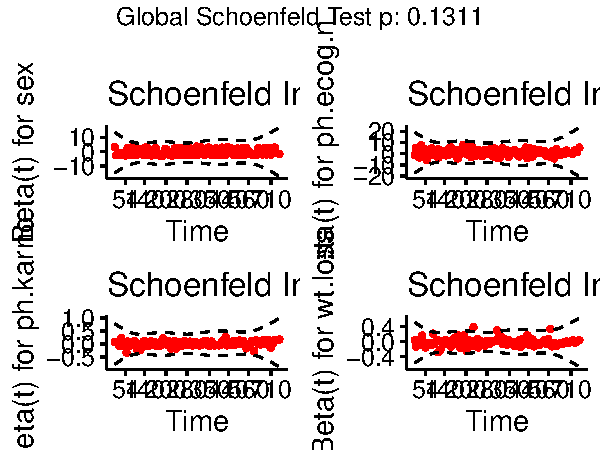
\includegraphics{final_project_files/figure-latex/unnamed-chunk-32-1.pdf}

\hypertarget{graphical-approach---log-log-curves}{%
\subsubsection{6.2 Graphical Approach - log-log
curves}\label{graphical-approach---log-log-curves}}

\hypertarget{sex-1}{%
\subsubsection{6.2.1 Sex}\label{sex-1}}

\begin{Shaded}
\begin{Highlighting}[]
\NormalTok{gplots }\OtherTok{\textless{}{-}} \FunctionTok{list}\NormalTok{()}

\NormalTok{test\_sex }\OtherTok{\textless{}{-}} \FunctionTok{survfit}\NormalTok{(}\FunctionTok{Surv}\NormalTok{(time, status }\SpecialCharTok{==} \DecValTok{1}\NormalTok{) }\SpecialCharTok{\textasciitilde{}}\NormalTok{ sex, }\AttributeTok{data =}\NormalTok{ lung\_mod)}

\NormalTok{gplots[[}\DecValTok{1}\NormalTok{]] }\OtherTok{=} \FunctionTok{ggsurvplot}\NormalTok{(test\_sex, }
           \AttributeTok{fun =} \StringTok{"cloglog"}\NormalTok{,}
           \AttributeTok{ggtheme =} \FunctionTok{theme\_bw}\NormalTok{(), }
           \AttributeTok{xlim =} \FunctionTok{c}\NormalTok{(}\DecValTok{5}\NormalTok{, }\DecValTok{1200}\NormalTok{),}
           \AttributeTok{legend =} \StringTok{"bottom"}\NormalTok{, }
           \AttributeTok{legend.title =} \StringTok{"Sex"}\NormalTok{,}
           \AttributeTok{legend.lab =} \FunctionTok{c}\NormalTok{(}\StringTok{"Male"}\NormalTok{, }\StringTok{"Female"}\NormalTok{),}
           \AttributeTok{xlab =} \StringTok{"log(Time)"}\NormalTok{,}
           \AttributeTok{ylab =} \StringTok{"log[{-}log(Survival Probability)]"}\NormalTok{)}
\end{Highlighting}
\end{Shaded}

\hypertarget{ecog-performance-score-1}{%
\subsubsection{6.2.2 ECOG performance
score}\label{ecog-performance-score-1}}

\begin{Shaded}
\begin{Highlighting}[]
\NormalTok{test\_ecog }\OtherTok{\textless{}{-}} \FunctionTok{survfit}\NormalTok{(}\FunctionTok{Surv}\NormalTok{(time, status }\SpecialCharTok{==} \DecValTok{1}\NormalTok{) }\SpecialCharTok{\textasciitilde{}}\NormalTok{ ph.ecog.n, }\AttributeTok{data =}\NormalTok{ lung\_mod)}

\NormalTok{gplots[[}\DecValTok{2}\NormalTok{]] }\OtherTok{=} \FunctionTok{ggsurvplot}\NormalTok{(test\_ecog, }
           \AttributeTok{fun =} \StringTok{"cloglog"}\NormalTok{,}
           \AttributeTok{ggtheme =} \FunctionTok{theme\_bw}\NormalTok{(),}
           \AttributeTok{xlim =} \FunctionTok{c}\NormalTok{(}\DecValTok{5}\NormalTok{, }\DecValTok{1200}\NormalTok{),}
           \AttributeTok{legend =} \StringTok{"bottom"}\NormalTok{, }
           \AttributeTok{legend.title =} \StringTok{"ECOG Performance Score"}\NormalTok{,}
           \AttributeTok{legend.lab =} \FunctionTok{c}\NormalTok{(}\StringTok{"0"}\NormalTok{, }\StringTok{"1"}\NormalTok{, }\StringTok{"2"}\NormalTok{),}
           \AttributeTok{xlab =} \StringTok{"log(Time)"}\NormalTok{,}
           \AttributeTok{ylab =} \StringTok{"log[{-}log(Survival Probability)]"}\NormalTok{)}
\end{Highlighting}
\end{Shaded}

\begin{Shaded}
\begin{Highlighting}[]
\CommentTok{\# combine the plots}
\FunctionTok{arrange\_ggsurvplots}\NormalTok{(gplots, }
                    \AttributeTok{print =} \ConstantTok{TRUE}\NormalTok{,}
                    \AttributeTok{title =} \StringTok{"Log of Negative Log of Estimated Survival Functions"}\NormalTok{,}
                    \AttributeTok{ncol =} \DecValTok{2}\NormalTok{, }
                    \AttributeTok{nrow =} \DecValTok{1}\NormalTok{)}
\end{Highlighting}
\end{Shaded}

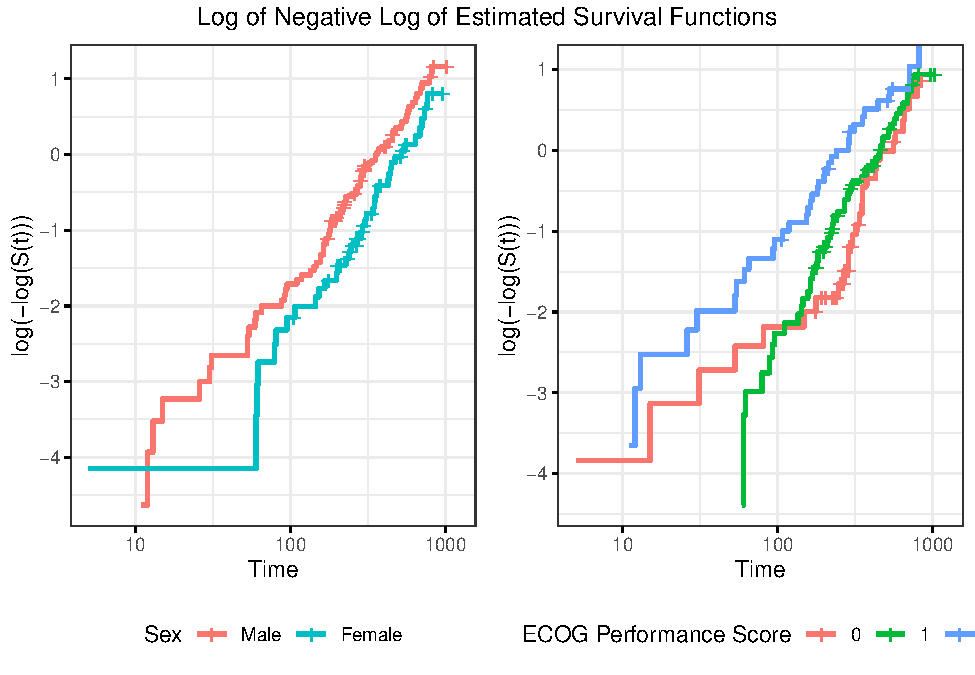
\includegraphics{final_project_files/figure-latex/unnamed-chunk-35-1.pdf}

\hypertarget{graphical-methods-observed-vs-fitted}{%
\subsection{Graphical methods -- observed vs
fitted}\label{graphical-methods-observed-vs-fitted}}

\hypertarget{ecog}{%
\subsubsection{ecog}\label{ecog}}

\begin{Shaded}
\begin{Highlighting}[]
\NormalTok{test\_ph\_ecog }\OtherTok{\textless{}{-}} \FunctionTok{coxph}\NormalTok{(}\FunctionTok{Surv}\NormalTok{(time, status }\SpecialCharTok{==} \DecValTok{1}\NormalTok{) }\SpecialCharTok{\textasciitilde{}}\NormalTok{ ph.ecog.n, lung\_mod)}

\FunctionTok{plot}\NormalTok{(test\_ecog, }\AttributeTok{col =} \FunctionTok{c}\NormalTok{(}\StringTok{"\#661100"}\NormalTok{,}\StringTok{"\#117733"}\NormalTok{, }\StringTok{"\#332288"}\NormalTok{),}
     \AttributeTok{xlab =} \StringTok{"Time (days)"}\NormalTok{, }\AttributeTok{ylab =} \StringTok{"Survival Function"}\NormalTok{,}
     \AttributeTok{main =} \StringTok{"Observed vs. Fitted"}\NormalTok{)}
\FunctionTok{lines}\NormalTok{(}\FunctionTok{survfit}\NormalTok{(test\_ph\_ecog, }\AttributeTok{newdata =} \FunctionTok{data.frame}\NormalTok{(}\AttributeTok{ph.ecog.n =} \FunctionTok{as.factor}\NormalTok{(}\DecValTok{0}\NormalTok{))), }\CommentTok{\# male}
      \AttributeTok{col =} \StringTok{"\#CC6677"}\NormalTok{, }\AttributeTok{conf.int =} \ConstantTok{FALSE}\NormalTok{)}
\FunctionTok{lines}\NormalTok{(}\FunctionTok{survfit}\NormalTok{(test\_ph\_ecog, }\AttributeTok{newdata =} \FunctionTok{data.frame}\NormalTok{(}\AttributeTok{ph.ecog.n =} \FunctionTok{as.factor}\NormalTok{(}\DecValTok{1}\NormalTok{))), }\CommentTok{\# female}
      \AttributeTok{col =} \StringTok{"\#999933"}\NormalTok{, }\AttributeTok{conf.int =} \ConstantTok{FALSE}\NormalTok{)}
\FunctionTok{lines}\NormalTok{(}\FunctionTok{survfit}\NormalTok{(test\_ph\_ecog, }\AttributeTok{newdata =} \FunctionTok{data.frame}\NormalTok{(}\AttributeTok{ph.ecog.n =} \FunctionTok{as.factor}\NormalTok{(}\DecValTok{2}\NormalTok{))), }\CommentTok{\# female}
      \AttributeTok{col =} \StringTok{"\#6699CC"}\NormalTok{, }\AttributeTok{conf.int =} \ConstantTok{FALSE}\NormalTok{)}
\FunctionTok{legend}\NormalTok{(}\StringTok{"topright"}\NormalTok{, }\AttributeTok{legend =} \FunctionTok{c}\NormalTok{(}\StringTok{"Observed ph.ecog = 0"}\NormalTok{, }\StringTok{"Fitted ph.ecog = 0"}\NormalTok{,}
                              \StringTok{"Observed ph.ecog = 1"}\NormalTok{, }\StringTok{"Fitted ph.ecog = 1"}\NormalTok{,}
                              \StringTok{"Observed ph.ecog = 2"}\NormalTok{, }\StringTok{"Fitted ph.ecog = 2"}\NormalTok{), }
       \AttributeTok{col =} \FunctionTok{c}\NormalTok{(}\StringTok{"\#661100"}\NormalTok{, }\StringTok{"\#CC6677"}\NormalTok{, }\StringTok{"\#117733"}\NormalTok{, }\StringTok{"\#999933"}\NormalTok{, }\StringTok{"\#332288"}\NormalTok{, }\StringTok{"\#6699CC"}\NormalTok{), }\AttributeTok{lty =} \DecValTok{1}\NormalTok{, }\AttributeTok{cex =} \FloatTok{0.65}\NormalTok{)}
\end{Highlighting}
\end{Shaded}

\includegraphics{final_project_files/figure-latex/unnamed-chunk-36-1.pdf}

\hypertarget{test-interaction-for-proportionality}{%
\subsubsection{6.3 Test interaction for
proportionality}\label{test-interaction-for-proportionality}}

\begin{Shaded}
\begin{Highlighting}[]
\NormalTok{cox\_mod\_5 }\OtherTok{=} \FunctionTok{coxph}\NormalTok{(}\FunctionTok{Surv}\NormalTok{(time, status }\SpecialCharTok{==} \DecValTok{1}\NormalTok{) }\SpecialCharTok{\textasciitilde{}}\NormalTok{ sex }\SpecialCharTok{+}\NormalTok{ ph.ecog.n }\SpecialCharTok{+}\NormalTok{ ph.karno }\SpecialCharTok{+}\NormalTok{ wt.loss }\SpecialCharTok{+}
\NormalTok{                  sex}\SpecialCharTok{*}\FunctionTok{log}\NormalTok{(time) }\SpecialCharTok{+}\NormalTok{ ph.ecog.n}\SpecialCharTok{*}\FunctionTok{log}\NormalTok{(time) }\SpecialCharTok{+}\NormalTok{ ph.karno}\SpecialCharTok{*}\FunctionTok{log}\NormalTok{(time)  }\SpecialCharTok{+}\NormalTok{ wt.loss}\SpecialCharTok{*}\FunctionTok{log}\NormalTok{(time) }
                  \SpecialCharTok{{-}} \FunctionTok{log}\NormalTok{(time), }
\NormalTok{                  lung\_mod) }
\FunctionTok{summary}\NormalTok{(cox\_mod\_5)}
\end{Highlighting}
\end{Shaded}

\begin{verbatim}
## Call:
## coxph(formula = Surv(time, status == 1) ~ sex + ph.ecog.n + ph.karno + 
##     wt.loss + sex * log(time) + ph.ecog.n * log(time) + ph.karno * 
##     log(time) + wt.loss * log(time) - log(time), data = lung_mod)
## 
##   n= 167, number of events= 120 
## 
##                            coef  exp(coef)   se(coef)         z Pr(>|z|)    
## sex2                 -1.413e+00  2.435e-01  3.567e-01    -3.961 7.47e-05 ***
## ph.ecog.n1           -5.475e-01  5.784e-01  3.381e-01    -1.619   0.1054    
## ph.ecog.n2            9.108e-02  1.095e+00  3.580e-01     0.254   0.7992    
## ph.karno             -5.613e-03  9.944e-01  1.375e-02    -0.408   0.6831    
## wt.loss               7.732e-02  1.080e+00  1.201e-02     6.439 1.20e-10 ***
## sex1:log(time)       -1.734e+02  5.128e-76  6.256e-02 -2771.127  < 2e-16 ***
## sex2:log(time)       -1.731e+02  6.582e-76  6.255e-02 -2767.407  < 2e-16 ***
## ph.ecog.n1:log(time)  1.003e-01  1.105e+00  6.090e-02     1.646   0.0997 .  
## ph.ecog.n2:log(time) -6.616e-02  9.360e-01  6.606e-02    -1.002   0.3166    
## ph.karno:log(time)   -3.481e-03  9.965e-01  2.413e-03    -1.442   0.1492    
## wt.loss:log(time)    -1.402e-02  9.861e-01  2.130e-03    -6.581 4.68e-11 ***
## ---
## Signif. codes:  0 '***' 0.001 '**' 0.01 '*' 0.05 '.' 0.1 ' ' 1
## 
##                      exp(coef) exp(-coef) lower .95 upper .95
## sex2                 2.435e-01  4.107e+00 1.210e-01 4.899e-01
## ph.ecog.n1           5.784e-01  1.729e+00 2.982e-01 1.122e+00
## ph.ecog.n2           1.095e+00  9.129e-01 5.430e-01 2.209e+00
## ph.karno             9.944e-01  1.006e+00 9.680e-01 1.022e+00
## wt.loss              1.080e+00  9.256e-01 1.055e+00 1.106e+00
## sex1:log(time)       5.128e-76  1.950e+75 4.537e-76 5.797e-76
## sex2:log(time)       6.582e-76  1.519e+75 5.822e-76 7.440e-76
## ph.ecog.n1:log(time) 1.105e+00  9.046e-01 9.811e-01 1.246e+00
## ph.ecog.n2:log(time) 9.360e-01  1.068e+00 8.223e-01 1.065e+00
## ph.karno:log(time)   9.965e-01  1.003e+00 9.918e-01 1.001e+00
## wt.loss:log(time)    9.861e-01  1.014e+00 9.820e-01 9.902e-01
## 
## Concordance= 1  (se = 0 )
## Likelihood ratio test= 948.8  on 11 df,   p=<2e-16
## Wald test            = 15337797  on 11 df,   p=<2e-16
## Score (logrank) test = 418.3  on 11 df,   p=<2e-16
\end{verbatim}

\hypertarget{correction-for-violation-of-ph-assumption}{%
\subsubsection{6.4 Correction for violation of PH
assumption}\label{correction-for-violation-of-ph-assumption}}

\hypertarget{stratified-ph-model}{%
\subsubsection{6.4.1 Stratified PH model}\label{stratified-ph-model}}

\begin{Shaded}
\begin{Highlighting}[]
\NormalTok{cox\_mod\_5 }\OtherTok{=} \FunctionTok{coxph}\NormalTok{(}\FunctionTok{Surv}\NormalTok{(time, status}\SpecialCharTok{==}\DecValTok{1}\NormalTok{) }\SpecialCharTok{\textasciitilde{}}\NormalTok{ (sex }\SpecialCharTok{+}\NormalTok{ wt.loss)}\SpecialCharTok{:} \FunctionTok{strata}\NormalTok{(ph.ecog.n) }\SpecialCharTok{+}\NormalTok{ ph.karno, lung\_mod) }
\FunctionTok{summary}\NormalTok{(cox\_mod\_5)}
\end{Highlighting}
\end{Shaded}

\begin{verbatim}
## Call:
## coxph(formula = Surv(time, status == 1) ~ (sex + wt.loss):strata(ph.ecog.n) + 
##     ph.karno, data = lung_mod)
## 
##   n= 167, number of events= 120 
## 
##                                  coef  exp(coef)   se(coef)      z Pr(>|z|)    
## ph.karno                    0.0207983  1.0210161  0.0119474  1.741 0.081715 .  
## sex1:strata(ph.ecog.n)0     1.0436802  2.8396484  0.4985491  2.093 0.036310 *  
## sex2:strata(ph.ecog.n)0            NA         NA  0.0000000     NA       NA    
## sex1:strata(ph.ecog.n)1     0.4530327  1.5730756  0.2773132  1.634 0.102332    
## sex2:strata(ph.ecog.n)1            NA         NA  0.0000000     NA       NA    
## sex1:strata(ph.ecog.n)2     1.4302644  4.1798043  0.4633990  3.086 0.002026 ** 
## sex2:strata(ph.ecog.n)2            NA         NA  0.0000000     NA       NA    
## wt.loss:strata(ph.ecog.n)0  0.0489525  1.0501705  0.0211402  2.316 0.020579 *  
## wt.loss:strata(ph.ecog.n)1 -0.0007336  0.9992667  0.0085458 -0.086 0.931589    
## wt.loss:strata(ph.ecog.n)2 -0.0667492  0.9354298  0.0172058 -3.879 0.000105 ***
## ---
## Signif. codes:  0 '***' 0.001 '**' 0.01 '*' 0.05 '.' 0.1 ' ' 1
## 
##                            exp(coef) exp(-coef) lower .95 upper .95
## ph.karno                      1.0210     0.9794    0.9974    1.0452
## sex1:strata(ph.ecog.n)0       2.8396     0.3522    1.0688    7.5445
## sex2:strata(ph.ecog.n)0           NA         NA        NA        NA
## sex1:strata(ph.ecog.n)1       1.5731     0.6357    0.9135    2.7089
## sex2:strata(ph.ecog.n)1           NA         NA        NA        NA
## sex1:strata(ph.ecog.n)2       4.1798     0.2392    1.6854   10.3658
## sex2:strata(ph.ecog.n)2           NA         NA        NA        NA
## wt.loss:strata(ph.ecog.n)0    1.0502     0.9522    1.0075    1.0946
## wt.loss:strata(ph.ecog.n)1    0.9993     1.0007    0.9827    1.0161
## wt.loss:strata(ph.ecog.n)2    0.9354     1.0690    0.9044    0.9675
## 
## Concordance= 0.613  (se = 0.033 )
## Likelihood ratio test= 32.68  on 7 df,   p=3e-05
## Wald test            = 28.91  on 7 df,   p=2e-04
## Score (logrank) test = 30.78  on 7 df,   p=7e-05
\end{verbatim}

\begin{Shaded}
\begin{Highlighting}[]
\FunctionTok{AIC}\NormalTok{(cox\_mod\_5)}
\end{Highlighting}
\end{Shaded}

\begin{verbatim}
## [1] 744.2391
\end{verbatim}

\begin{Shaded}
\begin{Highlighting}[]
\FunctionTok{BIC}\NormalTok{(cox\_mod\_5)}
\end{Highlighting}
\end{Shaded}

\begin{verbatim}
## [1] 763.7516
\end{verbatim}

\begin{Shaded}
\begin{Highlighting}[]
\CommentTok{\# check residuals}
\FunctionTok{cox.zph}\NormalTok{(cox\_mod\_5)}
\end{Highlighting}
\end{Shaded}

\begin{verbatim}
##                           chisq df    p
## ph.karno                   1.49  1 0.22
## sex:strata(ph.ecog.n)      4.05  3 0.26
## wt.loss:strata(ph.ecog.n)  6.19  3 0.10
## GLOBAL                     9.36  7 0.23
\end{verbatim}

\hypertarget{time-varying-covariates}{%
\subsubsection{6.4.2 Time-varying
covariates}\label{time-varying-covariates}}

\begin{Shaded}
\begin{Highlighting}[]
\CommentTok{\# explore ph.karno}
\NormalTok{cox\_karno }\OtherTok{=} \FunctionTok{coxph}\NormalTok{(}\FunctionTok{Surv}\NormalTok{(time, status}\SpecialCharTok{==}\DecValTok{1}\NormalTok{) }\SpecialCharTok{\textasciitilde{}}\NormalTok{ ph.karno, }\AttributeTok{data =}\NormalTok{ lung\_mod)}
\NormalTok{zph }\OtherTok{=} \FunctionTok{cox.zph}\NormalTok{(cox\_karno)}

\FunctionTok{plot}\NormalTok{(zph[}\DecValTok{1}\NormalTok{],}\AttributeTok{lwd=}\DecValTok{2}\NormalTok{) }
\FunctionTok{abline}\NormalTok{(}\DecValTok{0}\NormalTok{, }\DecValTok{0}\NormalTok{, }\AttributeTok{col=}\DecValTok{1}\NormalTok{,}\AttributeTok{lty=}\DecValTok{3}\NormalTok{,}\AttributeTok{lwd=}\DecValTok{2}\NormalTok{)}
\FunctionTok{abline}\NormalTok{(}\AttributeTok{h=}\NormalTok{ cox\_karno}\SpecialCharTok{$}\NormalTok{coef[}\DecValTok{1}\NormalTok{], }\AttributeTok{col=}\DecValTok{3}\NormalTok{, }\AttributeTok{lwd=}\DecValTok{2}\NormalTok{, }\AttributeTok{lty=}\DecValTok{2}\NormalTok{) }
\FunctionTok{legend}\NormalTok{(}\StringTok{"bottomright"}\NormalTok{,}
       \AttributeTok{legend=}\FunctionTok{c}\NormalTok{(}\StringTok{"Reference line for null effect"}\NormalTok{, }\StringTok{"Average hazard over time"}\NormalTok{, }\StringTok{"Time{-}varying hazard"}\NormalTok{),}
       \AttributeTok{lty=}\FunctionTok{c}\NormalTok{(}\DecValTok{3}\NormalTok{,}\DecValTok{2}\NormalTok{,}\DecValTok{1}\NormalTok{), }
       \AttributeTok{col=}\FunctionTok{c}\NormalTok{(}\DecValTok{1}\NormalTok{,}\DecValTok{3}\NormalTok{,}\DecValTok{1}\NormalTok{), }\AttributeTok{lwd=}\DecValTok{2}\NormalTok{)}
\end{Highlighting}
\end{Shaded}

\includegraphics{final_project_files/figure-latex/unnamed-chunk-39-1.pdf}

\begin{Shaded}
\begin{Highlighting}[]
\CommentTok{\# split the time period based on the plot}
\NormalTok{lung\_split }\OtherTok{=} \FunctionTok{survSplit}\NormalTok{(}\FunctionTok{Surv}\NormalTok{(time, status) }\SpecialCharTok{\textasciitilde{}}\NormalTok{ ., }\AttributeTok{data=}\NormalTok{ lung, }\AttributeTok{cut=}\FunctionTok{c}\NormalTok{(}\DecValTok{180}\NormalTok{, }\DecValTok{350}\NormalTok{), }\AttributeTok{episode=} \StringTok{"tgroup"}\NormalTok{, }\AttributeTok{id=}\StringTok{"id"}\NormalTok{)}

\NormalTok{cox\_mod\_6 }\OtherTok{=} \FunctionTok{coxph}\NormalTok{(}\FunctionTok{Surv}\NormalTok{(tstart, time, status) }\SpecialCharTok{\textasciitilde{}}\NormalTok{ sex }\SpecialCharTok{+}\NormalTok{ ph.ecog }\SpecialCharTok{+}\NormalTok{ ph.karno}\SpecialCharTok{:}\FunctionTok{strata}\NormalTok{(tgroup) }\SpecialCharTok{+}\NormalTok{ wt.loss, }\AttributeTok{data=}\NormalTok{lung\_split)}
\FunctionTok{summary}\NormalTok{(cox\_mod\_6)}
\end{Highlighting}
\end{Shaded}

\begin{verbatim}
## Call:
## coxph(formula = Surv(tstart, time, status) ~ sex + ph.ecog + 
##     ph.karno:strata(tgroup) + wt.loss, data = lung_split)
## 
##   n= 440, number of events= 151 
##    (21 observations deleted due to missingness)
## 
##                                      coef exp(coef)  se(coef)      z Pr(>|z|)
## sex                             -0.632406  0.531312  0.176582 -3.581 0.000342
## ph.ecog                          0.708542  2.031029  0.196019  3.615 0.000301
## wt.loss                         -0.008293  0.991741  0.006494 -1.277 0.201599
## ph.karno:strata(tgroup)tgroup=1 -0.007260  0.992767  0.013641 -0.532 0.594599
## ph.karno:strata(tgroup)tgroup=2  0.014597  1.014705  0.014090  1.036 0.300192
## ph.karno:strata(tgroup)tgroup=3  0.026358  1.026708  0.012689  2.077 0.037776
##                                    
## sex                             ***
## ph.ecog                         ***
## wt.loss                            
## ph.karno:strata(tgroup)tgroup=1    
## ph.karno:strata(tgroup)tgroup=2    
## ph.karno:strata(tgroup)tgroup=3 *  
## ---
## Signif. codes:  0 '***' 0.001 '**' 0.01 '*' 0.05 '.' 0.1 ' ' 1
## 
##                                 exp(coef) exp(-coef) lower .95 upper .95
## sex                                0.5313     1.8821    0.3759     0.751
## ph.ecog                            2.0310     0.4924    1.3831     2.982
## wt.loss                            0.9917     1.0083    0.9792     1.004
## ph.karno:strata(tgroup)tgroup=1    0.9928     1.0073    0.9666     1.020
## ph.karno:strata(tgroup)tgroup=2    1.0147     0.9855    0.9871     1.043
## ph.karno:strata(tgroup)tgroup=3    1.0267     0.9740    1.0015     1.053
## 
## Concordance= 0.647  (se = 0.027 )
## Likelihood ratio test= 36.18  on 6 df,   p=3e-06
## Wald test            = 35.42  on 6 df,   p=4e-06
## Score (logrank) test = 36.32  on 6 df,   p=2e-06
\end{verbatim}

\begin{Shaded}
\begin{Highlighting}[]
\FunctionTok{AIC}\NormalTok{(cox\_mod\_6)}
\end{Highlighting}
\end{Shaded}

\begin{verbatim}
## [1] 1325.87
\end{verbatim}

\begin{Shaded}
\begin{Highlighting}[]
\FunctionTok{BIC}\NormalTok{(cox\_mod\_6)}
\end{Highlighting}
\end{Shaded}

\begin{verbatim}
## [1] 1343.973
\end{verbatim}

\begin{Shaded}
\begin{Highlighting}[]
\CommentTok{\# check residuals}
\FunctionTok{cox.zph}\NormalTok{(cox\_mod\_6)}
\end{Highlighting}
\end{Shaded}

\begin{verbatim}
##                          chisq df    p
## sex                     2.0434  1 0.15
## ph.ecog                 0.2980  1 0.59
## wt.loss                 0.0386  1 0.84
## ph.karno:strata(tgroup) 3.2441  3 0.36
## GLOBAL                  5.6731  6 0.46
\end{verbatim}

\begin{Shaded}
\begin{Highlighting}[]
\CommentTok{\# The result shows now that there is no correlation between transformed survival time and the scaled Schoenfeld residuals, indicating that the proportional hazards assumption is not violated with the stratified analysis, and judging by the global p{-}value, the model is fit.}
\end{Highlighting}
\end{Shaded}

Consider AIC and BIC, we prefer model 5:\\
Surv(time, status) \textasciitilde{} (sex + wt.loss): strata(ph.ecog.n)
+ ph.karno. Also, stratified model is more flexible and powerful.

\hypertarget{parametric-model}{%
\subsection{7 Parametric Model}\label{parametric-model}}

\hypertarget{model-fitting}{%
\subsubsection{7.1 Model Fitting}\label{model-fitting}}

\begin{Shaded}
\begin{Highlighting}[]
\CommentTok{\# exponential}
\NormalTok{fit\_exp }\OtherTok{=} \FunctionTok{survreg}\NormalTok{(}\FunctionTok{Surv}\NormalTok{(time, status}\SpecialCharTok{==}\DecValTok{1}\NormalTok{) }\SpecialCharTok{\textasciitilde{}}\NormalTok{ sex }\SpecialCharTok{+}\NormalTok{ age }\SpecialCharTok{+}\NormalTok{ ph.ecog.n }\SpecialCharTok{+}\NormalTok{ ph.karno }\SpecialCharTok{+}\NormalTok{ pat.karno }\SpecialCharTok{+}\NormalTok{ meal.cal }\SpecialCharTok{+}\NormalTok{ wt.loss,}
                  \AttributeTok{data =}\NormalTok{ lung\_mod, }\AttributeTok{dist =} \StringTok{"exp"}\NormalTok{)}
\FunctionTok{summary}\NormalTok{(fit\_exp)}
\end{Highlighting}
\end{Shaded}

\begin{verbatim}
## 
## Call:
## survreg(formula = Surv(time, status == 1) ~ sex + age + ph.ecog.n + 
##     ph.karno + pat.karno + meal.cal + wt.loss, data = lung_mod, 
##     dist = "exp")
##                 Value Std. Error     z      p
## (Intercept)  7.55e+00   1.55e+00  4.88  1e-06
## sex2         5.16e-01   2.03e-01  2.54 0.0109
## age         -7.95e-03   1.14e-02 -0.70 0.4843
## ph.ecog.n1  -5.00e-01   2.79e-01 -1.79 0.0736
## ph.ecog.n2  -1.23e+00   4.56e-01 -2.69 0.0071
## ph.karno    -1.65e-02   1.14e-02 -1.45 0.1481
## pat.karno    7.55e-03   8.14e-03  0.93 0.3536
## meal.cal     4.79e-06   2.48e-04  0.02 0.9846
## wt.loss      9.98e-03   7.42e-03  1.35 0.1785
## 
## Scale fixed at 1 
## 
## Exponential distribution
## Loglik(model)= -837.2   Loglik(intercept only)= -848
##  Chisq= 21.63 on 8 degrees of freedom, p= 0.0057 
## Number of Newton-Raphson Iterations: 4 
## n= 167
\end{verbatim}

\begin{Shaded}
\begin{Highlighting}[]
\CommentTok{\# weibull}
\NormalTok{fit\_weibull }\OtherTok{=} \FunctionTok{survreg}\NormalTok{(}\FunctionTok{Surv}\NormalTok{(time, status}\SpecialCharTok{==}\DecValTok{1}\NormalTok{) }\SpecialCharTok{\textasciitilde{}}\NormalTok{ sex }\SpecialCharTok{+}\NormalTok{ age }\SpecialCharTok{+}\NormalTok{ ph.ecog.n }\SpecialCharTok{+}\NormalTok{ ph.karno }\SpecialCharTok{+}\NormalTok{ pat.karno }\SpecialCharTok{+}\NormalTok{ meal.cal }\SpecialCharTok{+}\NormalTok{ wt.loss,}
                      \AttributeTok{data =}\NormalTok{ lung\_mod, }\AttributeTok{dist =} \StringTok{"weibull"}\NormalTok{)}
\FunctionTok{summary}\NormalTok{(fit\_weibull)}
\end{Highlighting}
\end{Shaded}

\begin{verbatim}
## 
## Call:
## survreg(formula = Surv(time, status == 1) ~ sex + age + ph.ecog.n + 
##     ph.karno + pat.karno + meal.cal + wt.loss, data = lung_mod, 
##     dist = "weibull")
##                 Value Std. Error     z       p
## (Intercept)  7.36e+00   1.07e+00  6.86 6.7e-12
## sex2         3.97e-01   1.43e-01  2.78 0.00548
## age         -5.89e-03   8.07e-03 -0.73 0.46529
## ph.ecog.n1  -4.37e-01   1.96e-01 -2.23 0.02552
## ph.ecog.n2  -1.06e+00   3.18e-01 -3.33 0.00086
## ph.karno    -1.58e-02   7.64e-03 -2.06 0.03919
## pat.karno    7.31e-03   5.93e-03  1.23 0.21752
## meal.cal    -1.71e-05   1.79e-04 -0.10 0.92378
## wt.loss      9.43e-03   5.39e-03  1.75 0.08021
## Log(scale)  -3.55e-01   7.24e-02 -4.90 9.6e-07
## 
## Scale= 0.702 
## 
## Weibull distribution
## Loglik(model)= -827.1   Loglik(intercept only)= -841.1
##  Chisq= 27.9 on 8 degrees of freedom, p= 0.00049 
## Number of Newton-Raphson Iterations: 5 
## n= 167
\end{verbatim}

\begin{Shaded}
\begin{Highlighting}[]
\CommentTok{\# log{-}logistics}
\NormalTok{fit\_llogis }\OtherTok{=} \FunctionTok{survreg}\NormalTok{(}\FunctionTok{Surv}\NormalTok{(time, status}\SpecialCharTok{==}\DecValTok{1}\NormalTok{) }\SpecialCharTok{\textasciitilde{}}\NormalTok{ sex }\SpecialCharTok{+}\NormalTok{ age }\SpecialCharTok{+}\NormalTok{ ph.ecog.n }\SpecialCharTok{+}\NormalTok{ ph.karno }\SpecialCharTok{+}\NormalTok{ pat.karno }\SpecialCharTok{+}\NormalTok{ meal.cal }\SpecialCharTok{+}\NormalTok{ wt.loss,}
                     \AttributeTok{data =}\NormalTok{ lung\_mod, }\AttributeTok{dist =} \StringTok{"loglogistic"}\NormalTok{)}
\FunctionTok{summary}\NormalTok{(fit\_llogis)}
\end{Highlighting}
\end{Shaded}

\begin{verbatim}
## 
## Call:
## survreg(formula = Surv(time, status == 1) ~ sex + age + ph.ecog.n + 
##     ph.karno + pat.karno + meal.cal + wt.loss, data = lung_mod, 
##     dist = "loglogistic")
##                 Value Std. Error     z       p
## (Intercept)  5.786266   1.379040  4.20 2.7e-05
## sex2         0.504379   0.162349  3.11  0.0019
## age         -0.002170   0.008917 -0.24  0.8077
## ph.ecog.n1  -0.340770   0.225044 -1.51  0.1300
## ph.ecog.n2  -0.943484   0.404198 -2.33  0.0196
## ph.karno    -0.005662   0.011388 -0.50  0.6191
## pat.karno    0.006411   0.006220  1.03  0.3027
## meal.cal     0.000188   0.000196  0.96  0.3366
## wt.loss      0.006379   0.005533  1.15  0.2490
## Log(scale)  -0.651987   0.077160 -8.45 < 2e-16
## 
## Scale= 0.521 
## 
## Log logistic distribution
## Loglik(model)= -831.7   Loglik(intercept only)= -847
##  Chisq= 30.61 on 8 degrees of freedom, p= 0.00017 
## Number of Newton-Raphson Iterations: 4 
## n= 167
\end{verbatim}

\begin{Shaded}
\begin{Highlighting}[]
\CommentTok{\# log{-}normal}
\NormalTok{fit\_lnorm }\OtherTok{=} \FunctionTok{survreg}\NormalTok{(}\FunctionTok{Surv}\NormalTok{(time, status}\SpecialCharTok{==}\DecValTok{1}\NormalTok{) }\SpecialCharTok{\textasciitilde{}}\NormalTok{ sex }\SpecialCharTok{+}\NormalTok{ age }\SpecialCharTok{+}\NormalTok{ ph.ecog.n }\SpecialCharTok{+}\NormalTok{ ph.karno }\SpecialCharTok{+}\NormalTok{ pat.karno }\SpecialCharTok{+}\NormalTok{ meal.cal }\SpecialCharTok{+}\NormalTok{ wt.loss,}
                    \AttributeTok{data =}\NormalTok{ lung\_mod, }\AttributeTok{dist =} \StringTok{"lognormal"}\NormalTok{)}
\FunctionTok{summary}\NormalTok{(fit\_lnorm)}
\end{Highlighting}
\end{Shaded}

\begin{verbatim}
## 
## Call:
## survreg(formula = Surv(time, status == 1) ~ sex + age + ph.ecog.n + 
##     ph.karno + pat.karno + meal.cal + wt.loss, data = lung_mod, 
##     dist = "lognormal")
##                 Value Std. Error     z       p
## (Intercept)  6.903492   1.469556  4.70 2.6e-06
## sex2         0.491426   0.181341  2.71  0.0067
## age         -0.011962   0.010129 -1.18  0.2376
## ph.ecog.n1  -0.300961   0.252437 -1.19  0.2332
## ph.ecog.n2  -1.047816   0.425026 -2.47  0.0137
## ph.karno    -0.012873   0.011694 -1.10  0.2710
## pat.karno    0.006390   0.006855  0.93  0.3513
## meal.cal     0.000242   0.000219  1.11  0.2680
## wt.loss      0.007127   0.006297  1.13  0.2577
## Log(scale)  -0.002009   0.065457 -0.03  0.9755
## 
## Scale= 0.998 
## 
## Log Normal distribution
## Loglik(model)= -838.4   Loglik(intercept only)= -853.4
##  Chisq= 29.92 on 8 degrees of freedom, p= 0.00022 
## Number of Newton-Raphson Iterations: 4 
## n= 167
\end{verbatim}

\hypertarget{model-comparison-1}{%
\subsubsection{7.2 Model Comparison}\label{model-comparison-1}}

\begin{Shaded}
\begin{Highlighting}[]
\FunctionTok{AIC}\NormalTok{(fit\_exp, fit\_weibull, fit\_llogis, fit\_lnorm)}
\end{Highlighting}
\end{Shaded}

\begin{verbatim}
##             df      AIC
## fit_exp      9 1692.421
## fit_weibull 10 1674.235
## fit_llogis  10 1683.443
## fit_lnorm   10 1696.821
\end{verbatim}

\begin{Shaded}
\begin{Highlighting}[]
\FunctionTok{BIC}\NormalTok{(fit\_exp, fit\_weibull, fit\_llogis, fit\_lnorm)}
\end{Highlighting}
\end{Shaded}

\begin{verbatim}
##             df      BIC
## fit_exp      9 1720.483
## fit_weibull 10 1705.415
## fit_llogis  10 1714.623
## fit_lnorm   10 1728.001
\end{verbatim}

\begin{Shaded}
\begin{Highlighting}[]
\NormalTok{fit\_sex }\OtherTok{=} \FunctionTok{survfit}\NormalTok{(}\FunctionTok{Surv}\NormalTok{(time, status }\SpecialCharTok{==} \DecValTok{1}\NormalTok{) }\SpecialCharTok{\textasciitilde{}}\NormalTok{ sex, }\AttributeTok{data =}\NormalTok{ lung\_mod)}

\CommentTok{\# {-}log(S(t))}
\FunctionTok{ggsurvplot}\NormalTok{(fit\_sex, }
           \AttributeTok{fun =} \StringTok{"cumhaz"}\NormalTok{,}
           \AttributeTok{xlim =} \FunctionTok{c}\NormalTok{(}\DecValTok{5}\NormalTok{, }\DecValTok{1200}\NormalTok{),}
           \AttributeTok{title =} \StringTok{"Negative Log of Estimated Survival Functions"}\NormalTok{,}
           \AttributeTok{legend.lab =} \FunctionTok{c}\NormalTok{(}\StringTok{"Male"}\NormalTok{, }\StringTok{"Female"}\NormalTok{),}
           \AttributeTok{ggtheme =} \FunctionTok{theme\_bw}\NormalTok{())}
\end{Highlighting}
\end{Shaded}

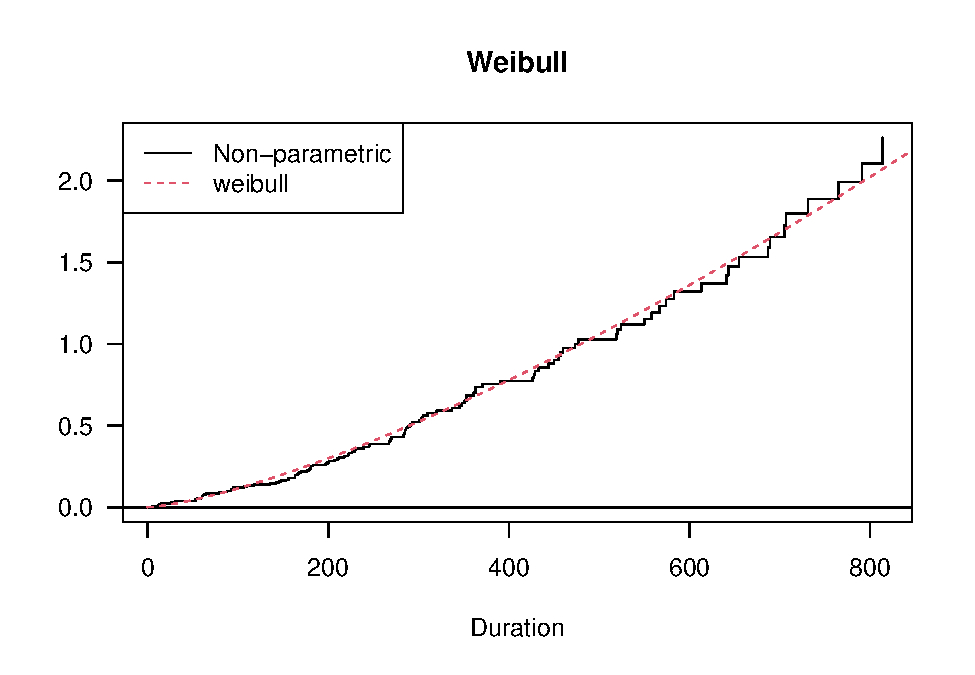
\includegraphics{final_project_files/figure-latex/unnamed-chunk-41-1.pdf}

\begin{Shaded}
\begin{Highlighting}[]
\CommentTok{\# log({-}log(S(t)))}
\FunctionTok{ggsurvplot}\NormalTok{(fit\_sex, }
           \AttributeTok{fun =} \StringTok{"cloglog"}\NormalTok{,}
           \AttributeTok{xlim =} \FunctionTok{c}\NormalTok{(}\DecValTok{5}\NormalTok{, }\DecValTok{1200}\NormalTok{),}
           \AttributeTok{title =} \StringTok{"Log of Negative Log of Estimated Survival Functions"}\NormalTok{,}
           \AttributeTok{legend.lab =} \FunctionTok{c}\NormalTok{(}\StringTok{"Male"}\NormalTok{, }\StringTok{"Female"}\NormalTok{),}
           \AttributeTok{ggtheme =} \FunctionTok{theme\_bw}\NormalTok{())}
\end{Highlighting}
\end{Shaded}

\includegraphics{final_project_files/figure-latex/unnamed-chunk-41-2.pdf}

\begin{Shaded}
\begin{Highlighting}[]
\CommentTok{\# Weibull is better}
\end{Highlighting}
\end{Shaded}

\hypertarget{model-selection}{%
\subsubsection{7.2 Model Selection}\label{model-selection}}

\begin{Shaded}
\begin{Highlighting}[]
\CommentTok{\# full weibull model}
\NormalTok{web }\OtherTok{=} \FunctionTok{psm}\NormalTok{(}\FunctionTok{Surv}\NormalTok{(time, status}\SpecialCharTok{==}\DecValTok{1}\NormalTok{) }\SpecialCharTok{\textasciitilde{}}\NormalTok{ sex }\SpecialCharTok{+}\NormalTok{ age }\SpecialCharTok{+}\NormalTok{ ph.ecog.n }\SpecialCharTok{+}\NormalTok{ ph.karno }\SpecialCharTok{+}\NormalTok{ pat.karno }\SpecialCharTok{+}\NormalTok{ meal.cal }\SpecialCharTok{+}\NormalTok{ wt.loss, }\AttributeTok{data =}\NormalTok{ lung\_mod)}

\CommentTok{\# backward selection}
\FunctionTok{fastbw}\NormalTok{(web, }\AttributeTok{rule=}\StringTok{"aic"}\NormalTok{)}
\end{Highlighting}
\end{Shaded}

\begin{verbatim}
## 
##  Deleted   Chi-Sq d.f. P      Residual d.f. P      AIC  
##  meal.cal  0.01   1    0.9238 0.01     1    0.9238 -1.99
##  age       0.52   1    0.4690 0.53     2    0.7659 -3.47
##  pat.karno 1.54   1    0.2140 2.08     3    0.5565 -3.92
##  wt.loss   2.55   1    0.1103 4.63     4    0.3277 -3.37
##  ph.karno  3.36   1    0.0669 7.99     5    0.1570 -2.01
## 
## Approximate Estimates after Deleting Factors
## 
##                Coef   S.E. Wald Z         P
## (Intercept)  6.1568 0.1395 44.146 0.0000000
## sex=2        0.3645 0.1400  2.603 0.0092423
## ph.ecog.n=1 -0.2169 0.1634 -1.327 0.1844536
## ph.ecog.n=2 -0.6838 0.1842 -3.713 0.0002047
## 
## Factors in Final Model
## 
## [1] sex       ph.ecog.n
\end{verbatim}

\begin{Shaded}
\begin{Highlighting}[]
\CommentTok{\# compare with cox model}
\NormalTok{web\_1 }\OtherTok{=} \FunctionTok{phreg}\NormalTok{(}\FunctionTok{Surv}\NormalTok{(time, status}\SpecialCharTok{==}\DecValTok{1}\NormalTok{) }\SpecialCharTok{\textasciitilde{}}\NormalTok{ sex }\SpecialCharTok{+}\NormalTok{ ph.ecog.n,}
                      \AttributeTok{data =}\NormalTok{ lung\_mod, }\AttributeTok{dist =} \StringTok{"weibull"}\NormalTok{)}
\NormalTok{cox\_1 }\OtherTok{=} \FunctionTok{coxreg}\NormalTok{(}\FunctionTok{Surv}\NormalTok{(time, status}\SpecialCharTok{==}\DecValTok{1}\NormalTok{) }\SpecialCharTok{\textasciitilde{}}\NormalTok{ sex }\SpecialCharTok{+}\NormalTok{ ph.ecog.n, }\AttributeTok{data =}\NormalTok{ lung\_mod)}

\FunctionTok{check.dist}\NormalTok{(web\_1, cox\_1)}
\end{Highlighting}
\end{Shaded}

\includegraphics{final_project_files/figure-latex/unnamed-chunk-42-1.pdf}

\begin{Shaded}
\begin{Highlighting}[]
\CommentTok{\# final model}
\NormalTok{web\_final }\OtherTok{=} \FunctionTok{survreg}\NormalTok{(}\FunctionTok{Surv}\NormalTok{(time, status}\SpecialCharTok{==}\DecValTok{1}\NormalTok{) }\SpecialCharTok{\textasciitilde{}}\NormalTok{ sex }\SpecialCharTok{+}\NormalTok{ ph.ecog.n,}
                      \AttributeTok{data =}\NormalTok{ lung\_mod, }\AttributeTok{dist =} \StringTok{"weibull"}\NormalTok{)}


\CommentTok{\# Scale parameter}
\NormalTok{web\_final}\SpecialCharTok{$}\NormalTok{scale}
\end{Highlighting}
\end{Shaded}

\begin{verbatim}
## [1] 0.7259592
\end{verbatim}

\begin{Shaded}
\begin{Highlighting}[]
\CommentTok{\# Shape parameter}
\NormalTok{(shapeParameter }\OtherTok{\textless{}{-}} \DecValTok{1} \SpecialCharTok{/}\NormalTok{ web\_final}\SpecialCharTok{$}\NormalTok{scale)}
\end{Highlighting}
\end{Shaded}

\begin{verbatim}
## [1] 1.377488
\end{verbatim}

\begin{Shaded}
\begin{Highlighting}[]
\DocumentationTok{\#\# AFT interpretation}
\FunctionTok{exp}\NormalTok{(}\FunctionTok{coef}\NormalTok{(web\_final))}
\end{Highlighting}
\end{Shaded}

\begin{verbatim}
## (Intercept)        sex2  ph.ecog.n1  ph.ecog.n2 
## 479.7465780   1.4499851   0.8098967   0.5040564
\end{verbatim}

\begin{Shaded}
\begin{Highlighting}[]
\DocumentationTok{\#\# Geometric mean of survival time: 479.747}
\DocumentationTok{\#\# female extends survival time by 1.45 times then male}
\DocumentationTok{\#\# ecog = 1 shortens survival time by 0.81 times than ecog = 0}
\DocumentationTok{\#\# ecog = 2 shortens survival time by 0.504 times than ecog = 0}
\end{Highlighting}
\end{Shaded}


\end{document}
